\section{Results and Discussion}
\label{sec:results}
\begin{figure*}[t]
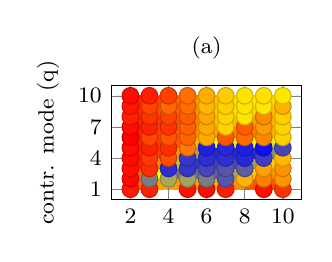
\begin{tikzpicture}
\begin{axis}
[
width=0.33\textwidth,
height=0.25\textwidth,
style={font=\footnotesize},
grid=major,
grid style={dotted},
align=center,
%xlabel={tensor order},
ylabel={contr. mode (q)},
title={{(a)}}, %  bgemm, asymmetric
scaled ticks=false,
zlabel={GFlops},
view={0}{90}, 
ytick={1,4,7,10},
xtick={2,4,6,8,10},
xmin=1, xmax=11,
ymin=0, ymax=11,
try min ticks=8,
zmin=300, zmax=2300,
point meta min=300, point meta max=2300,
colormap/hot, 
samples=50,
%colorbar sampled,
%colorbar/width=0.2cm,
%colorbar style={
%	point meta min=300, point meta max=2300,
%	samples=50,
%	font=\footnotesize,
%	ytick={300,1300,2300},
%	yticklabels={0.3,1.3,2.3},
%	%title={\scriptsize Gflops},
%	%ylabel={\scriptsize Gflops},
%}
]
%\addplot3[mesh, scatter,samples=50,shader=interp]
%\addplot3[only marks, mesh, scatter,scatter src=z,samples=50,] % z buffer=sort, scatter src=z,
\addplot3[contour filled={number=100},scatter,shader=flat,samples=50]
%\addplot3+[mesh,scatter,shader=flat corner,samples=50, only marks, mark size=2]
coordinates{
	
(2.000,1.000,2142.734) (2.000,2.000,2241.014) (2.000,3.000,2205.546) (2.000,4.000,2226.263) (2.000,5.000,2232.877) (2.000,6.000,2281.816) (2.000,7.000,2222.317) (2.000,8.000,2122.831) (2.000,9.000,2166.437) (2.000,10.000,2231.354) 

(3.000,1.000,2104.803) (3.000,2.000,620.292) (3.000,3.000,2053.810) (3.000,4.000,1989.460) (3.000,5.000,2100.108) (3.000,6.000,1923.866) (3.000,7.000,2109.798) (3.000,8.000,2032.918) (3.000,9.000,1931.835) (3.000,10.000,2137.550) 

(4.000,1.000,2303.560) (4.000,2.000,742.055) (4.000,3.000,436.752) (4.000,4.000,1889.266) (4.000,5.000,2050.848) (4.000,6.000,1845.429) (4.000,7.000,2029.757) (4.000,8.000,1947.246) (4.000,9.000,1753.968) (4.000,10.000,1945.836) 

(5.000,1.000,2197.949) (5.000,2.000,727.736) (5.000,3.000,441.734) (5.000,4.000,458.055) (5.000,5.000,1643.657) (5.000,6.000,1763.676) (5.000,7.000,1793.195) (5.000,8.000,1799.906) (5.000,9.000,1726.622) (5.000,10.000,1710.693) 

(6.000,1.000,2225.857) (6.000,2.000,621.489) (6.000,3.000,489.438) (6.000,4.000,435.500) (6.000,5.000,386.554) (6.000,6.000,1410.907) (6.000,7.000,1419.437) (6.000,8.000,1428.795) (6.000,9.000,1330.280) (6.000,10.000,1386.923) 

(7.000,1.000,2137.668) (7.000,2.000,530.662) (7.000,3.000,532.587) (7.000,4.000,439.307) (7.000,5.000,400.923) (7.000,6.000,1835.402) (7.000,7.000,1186.143) (7.000,8.000,1195.514) (7.000,9.000,1211.432) (7.000,10.000,1230.143) 

(8.000,1.000,2411.000) (8.000,2.000,1340.829) (8.000,3.000,546.729) (8.000,4.000,405.255) (8.000,5.000,381.061) (8.000,6.000,1724.053) (8.000,7.000,1816.684) (8.000,8.000,1103.276) (8.000,9.000,1109.365) (8.000,10.000,1119.582) 

(9.000,1.000,2215.896) (9.000,2.000,1637.409) (9.000,3.000,1448.314) (9.000,4.000,477.752) (9.000,5.000,353.959) (9.000,6.000,1596.361) (9.000,7.000,1496.308) (9.000,8.000,1566.431) (9.000,9.000,1085.107) (9.000,10.000,1135.908) 

(10.000,1.000,2011.147) (10.000,2.000,1504.412) (10.000,3.000,1538.421) (10.000,4.000,1335.732) (10.000,5.000,483.993) (10.000,6.000,1202.734) (10.000,7.000,1197.316) (10.000,8.000,1213.834) (10.000,9.000,1362.208) (10.000,10.000,1087.708)


};
\end{axis}
\end{tikzpicture}
\hfill
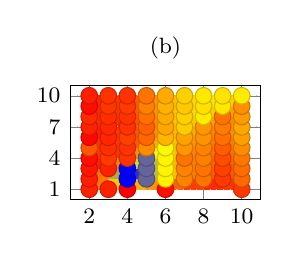
\begin{tikzpicture}
\begin{axis}
[
width=0.33\textwidth,
height=0.25\textwidth,
style={font=\footnotesize},
grid=major,
grid style={dotted},
align=center,
%xlabel={tensor order},
%ylabel={contr. mode (q)},
title={{(b)}}, %  ompfor<2d-slice> ttm<par-loops,seq-blas,$q$-slice>, asymmetric
scaled ticks=false,
zlabel={GFlops},
view={0}{90}, 
%view={-45}{45}, 
ytick={1,4,7,10},
xtick={2,4,6,8,10},
xmin=1, xmax=11,
ymin=0, ymax=11,
try min ticks=8,
zmin=300, zmax=2300,
point meta min=300, point meta max=2300,
colormap/hot, 
samples=50,
%colorbar sampled,
%colorbar/width=0.2cm,
%colorbar style={
%	point meta min=300, point meta max=2300,
%	samples=50,
%	font=\footnotesize,
%	ytick={300,1300,2300},
%	yticklabels={0.3,1.3,2.3},
%	%title={\scriptsize Gflops},
%	%ylabel={\scriptsize Gflops},
%}
]
%\addplot3[mesh, scatter,samples=50,shader=interp]
%\addplot3[only marks, mesh, scatter,scatter src=z,samples=50,] % z buffer=sort, scatter src=z,
\addplot3[contour filled={number=100},scatter,shader=flat,samples=50]
%\addplot3+[mesh,scatter,shader=flat corner,samples=50, only marks, mark size=2]
coordinates{

(2.000,1.000,2107.002) (2.000,2.000,2127.162) (2.000,3.000,2176.298) (2.000,4.000,2215.649) (2.000,5.000,1837.632) (2.000,6.000,2241.609) (2.000,7.000,2101.558) (2.000,8.000,2075.436) (2.000,9.000,2236.130) (2.000,10.000,2133.353) 

(3.000,1.000,2119.523) (3.000,2.000,167.437) (3.000,3.000,2112.420) (3.000,4.000,1989.285) (3.000,5.000,2041.921) (3.000,6.000,2084.201) (3.000,7.000,2080.454) (3.000,8.000,2046.614) (3.000,9.000,2013.009) (3.000,10.000,2024.421) 

(4.000,1.000,2285.299) (4.000,2.000,314.287) (4.000,3.000,311.849) (4.000,4.000,2011.869) (4.000,5.000,2039.029) (4.000,6.000,1944.642) (4.000,7.000,2023.178) (4.000,8.000,2033.385) (4.000,9.000,1992.379) (4.000,10.000,2039.303) 

(5.000,1.000,2475.804) (5.000,2.000,568.291) (5.000,3.000,562.230) (5.000,4.000,562.587) (5.000,5.000,1564.667) (5.000,6.000,1756.890) (5.000,7.000,1791.524) (5.000,8.000,1712.024) (5.000,9.000,1626.887) (5.000,10.000,1695.764) 

(6.000,1.000,2218.038) (6.000,2.000,1025.980) (6.000,3.000,1034.039) (6.000,4.000,1026.350) (6.000,5.000,945.367) (6.000,6.000,1340.191) (6.000,7.000,1422.937) (6.000,8.000,1402.244) (6.000,9.000,1375.707) (6.000,10.000,1411.432) 

(7.000,1.000,2307.246) (7.000,2.000,1602.074) (7.000,3.000,1617.348) (7.000,4.000,1682.539) (7.000,5.000,1516.443) (7.000,6.000,1446.511) (7.000,7.000,1229.353) (7.000,8.000,1202.606) (7.000,9.000,1245.855) (7.000,10.000,1211.880) 

(8.000,1.000,2441.539) (8.000,2.000,1699.771) (8.000,3.000,1686.405) (8.000,4.000,1622.372) (8.000,5.000,1600.438) (8.000,6.000,1530.707) (8.000,7.000,1508.466) (8.000,8.000,1073.808) (8.000,9.000,1123.363) (8.000,10.000,1096.486) 

(9.000,1.000,2330.060) (9.000,2.000,1985.056) (9.000,3.000,1941.312) (9.000,4.000,1892.533) (9.000,5.000,1805.699) (9.000,6.000,1706.515) (9.000,7.000,1658.818) (9.000,8.000,1693.350) (9.000,9.000,1093.684) (9.000,10.000,1112.530) 

(10.000,1.000,1988.818) (10.000,2.000,1750.516) (10.000,3.000,1728.226) (10.000,4.000,1678.568) (10.000,5.000,1576.395) (10.000,6.000,1476.492) (10.000,7.000,1429.733) (10.000,8.000,1496.574) (10.000,9.000,1557.162) (10.000,10.000,1068.719) 


};
\end{axis}
\end{tikzpicture}
\hfill
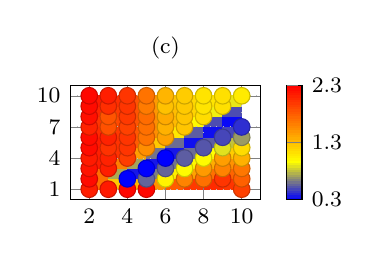
\begin{tikzpicture}
\begin{axis}
[
width=0.33\textwidth,
height=0.25\textwidth,
style={font=\footnotesize},
grid=major,
grid style={dotted},
align=center,
%xlabel={tensor order},
%ylabel={contr. mode (q)},
title={{(c)}}, %  ompfor<qd-slice> ttm<par-loops,seq-blas,$q$-slice>, asymmetric
scaled ticks=false,
zlabel={GFlops},
view={0}{90}, 
%view={-45}{45}, 
ytick={1,4,7,10},
xtick={2,4,6,8,10},
%xmin=2, xmax=10,
%ymin=1, ymax=10,
xmin=1, xmax=11,
ymin=0, ymax=11,
try min ticks=8,
zmin=300, zmax=2300,
point meta min=300, point meta max=2300,
%colormap/jet, 
colormap/hot, 
%colormap/blackwhite,
%colormap={whiteblack}{indices of colormap={\pgfplotscolormaplastindexof{blackwhite},...,0 of blackwhite}},
samples=50,
%colormap access=piecewise const,
colorbar sampled,
colorbar/width=0.2cm,
colorbar style={
	point meta min=300, point meta max=2300,
	samples=50,
	font=\footnotesize,
	ytick={300,1300,2300},
	yticklabels={0.3,1.3,2.3},
	%title={\scriptsize Gflops},
	%ylabel={\scriptsize Gflops},
}
]
%\addplot3[mesh, scatter,samples=50,shader=interp]
%\addplot3[only marks, mesh, scatter,scatter src=z,samples=50,] % z buffer=sort, scatter src=z,
\addplot3[contour filled={number=100},scatter,shader=flat,samples=50]
%\addplot3+[mesh,scatter,shader=flat corner,samples=50, only marks, mark size=2]
coordinates{

(2.000,1.000,2134.021) (2.000,2.000,2224.864) (2.000,3.000,2184.477) (2.000,4.000,2142.541) (2.000,5.000,2229.439) (2.000,6.000,2238.772) (2.000,7.000,2105.091) (2.000,8.000,2201.214) (2.000,9.000,2232.448) (2.000,10.000,2240.926) 

(3.000,1.000,2146.896) (3.000,2.000,167.544) (3.000,3.000,2121.476) (3.000,4.000,2105.304) (3.000,5.000,2027.717) (3.000,6.000,2104.722) (3.000,7.000,1866.561) (3.000,8.000,1855.180) (3.000,9.000,2041.894) (3.000,10.000,2122.692) 

(4.000,1.000,2244.985) (4.000,2.000,313.766) (4.000,3.000,167.879) (4.000,4.000,1973.457) (4.000,5.000,2013.391) (4.000,6.000,2010.678) (4.000,7.000,1949.136) (4.000,8.000,1989.844) (4.000,9.000,2017.192) (4.000,10.000,2015.899) 

(5.000,1.000,2250.694) (5.000,2.000,574.277) (5.000,3.000,315.908) (5.000,4.000,166.343) (5.000,5.000,1559.782) (5.000,6.000,1688.138) (5.000,7.000,1711.412) (5.000,8.000,1721.389) (5.000,9.000,1653.587) (5.000,10.000,1691.902) 

(6.000,1.000,2403.465) (6.000,2.000,1026.371) (6.000,3.000,576.699) (6.000,4.000,312.020) (6.000,5.000,160.917) (6.000,6.000,1443.174) (6.000,7.000,1370.699) (6.000,8.000,1414.204) (6.000,9.000,1283.900) (6.000,10.000,1351.446) 

(7.000,1.000,2305.894) (7.000,2.000,1613.830) (7.000,3.000,988.435) (7.000,4.000,554.792) (7.000,5.000,290.305) (7.000,6.000,157.356) (7.000,7.000,1270.432) (7.000,8.000,1266.914) (7.000,9.000,1255.620) (7.000,10.000,1224.914) 

(8.000,1.000,2437.239) (8.000,2.000,1706.219) (8.000,3.000,1489.110) (8.000,4.000,999.755) (8.000,5.000,531.137) (8.000,6.000,280.182) (8.000,7.000,148.892) (8.000,8.000,1156.621) (8.000,9.000,1110.478) (8.000,10.000,1116.944) 

(9.000,1.000,2355.395) (9.000,2.000,2003.839) (9.000,3.000,1603.752) (9.000,4.000,1477.309) (9.000,5.000,887.839) (9.000,6.000,492.554) (9.000,7.000,262.294) (9.000,8.000,150.408) (9.000,9.000,1129.997) (9.000,10.000,1121.143) 

(10.000,1.000,1944.959) (10.000,2.000,1789.054) (10.000,3.000,1665.441) (10.000,4.000,1375.291) (10.000,5.000,1147.731) (10.000,6.000,715.205) (10.000,7.000,422.658) (10.000,8.000,236.076) (10.000,9.000,136.520) (10.000,10.000,1078.495) 


};
\end{axis}
\end{tikzpicture}


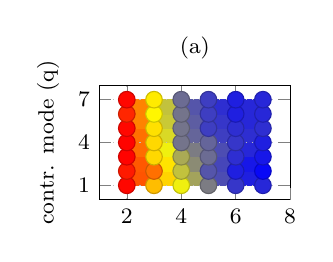
\begin{tikzpicture}
\begin{axis}
[
width=0.33\textwidth,
height=0.25\textwidth,
style={font=\footnotesize},
grid=major,
grid style={dotted},
align=center,
%xlabel={tensor order},
ylabel={contr. mode (q)},
title={{(a)}}, %  bgemm, asymmetric
scaled ticks=false,
zlabel={GFlops},
view={0}{90}, 
ytick={1,4,7,10},
xtick={2,4,6,8},
xmin=1, xmax=8,
ymin=0, ymax=8,
try min ticks=8,
zmin=0, zmax=2600,
point meta min=0, point meta max=2600,
colormap/hot, 
samples=50,
%colorbar sampled,
%colorbar/width=0.2cm,
%colorbar style={
%	point meta min=300, point meta max=2300,
%	samples=50,
%	font=\footnotesize,
%	ytick={300,1300,2300},
%	yticklabels={0.3,1.3,2.3},
%	%title={\scriptsize Gflops},
%	%ylabel={\scriptsize Gflops},
%}
]
%\addplot3[mesh, scatter,samples=50,shader=interp]
%\addplot3[only marks, mesh, scatter,scatter src=z,samples=50,] % z buffer=sort, scatter src=z,
\addplot3[contour filled={number=100},scatter,shader=flat,samples=50]
%\addplot3+[mesh,scatter,shader=flat corner,samples=50, only marks, mark size=2]
coordinates{

(2.000,1.000,2527.923) (2.000,2.000,2398.051) (2.000,3.000,2573.521) (2.000,4.000,2570.296) (2.000,5.000,2540.651) (2.000,6.000,2326.903) (2.000,7.000,2545.629) 

(3.000,1.000,1312.517) (3.000,2.000,1835.211) (3.000,3.000,1133.124) (3.000,4.000,1120.384) (3.000,5.000,1066.704) (3.000,6.000,915.932) (3.000,7.000,997.168) 

(4.000,1.000,825.045) (4.000,2.000,655.270) (4.000,3.000,579.750) (4.000,4.000,390.794) (4.000,5.000,411.134) (4.000,6.000,409.619) (4.000,7.000,375.457) 

(5.000,1.000,420.343) (5.000,2.000,308.678) (5.000,3.000,377.118) (5.000,4.000,348.232) (5.000,5.000,216.877) (5.000,6.000,232.073) (5.000,7.000,218.457) 

(6.000,1.000,206.774) (6.000,2.000,119.299) (6.000,3.000,167.691) (6.000,4.000,183.571) (6.000,5.000,179.989) (6.000,6.000,126.876) (6.000,7.000,128.135) 

(7.000,1.000,150.823) (7.000,2.000,33.170) (7.000,3.000,83.979) (7.000,4.000,128.221) (7.000,5.000,157.368) (7.000,6.000,143.557) (7.000,7.000,133.647) 


};
\end{axis}
\end{tikzpicture}
\hfill
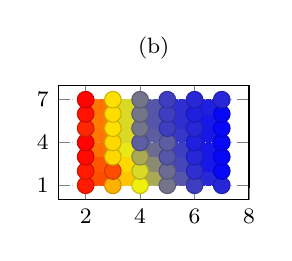
\begin{tikzpicture}
\begin{axis}
[
width=0.33\textwidth,
height=0.25\textwidth,
style={font=\footnotesize},
grid=major,
grid style={dotted},
align=center,
%xlabel={tensor order},
%ylabel={contr. mode (q)},
title={{(b)}}, %  ompfor<2d-slice> ttm<par-loops,seq-blas,$q$-slice>, asymmetric
scaled ticks=false,
zlabel={GFlops},
view={0}{90}, 
%view={-45}{45}, 
ytick={1,4,7,10},
xtick={2,4,6,8},
xmin=1, xmax=8,
ymin=0, ymax=8,
try min ticks=8,
zmin=0, zmax=2600,
point meta min=0, point meta max=2600,
colormap/hot, 
samples=50,
%colorbar sampled,
%colorbar/width=0.2cm,
%colorbar style={
%	point meta min=300, point meta max=2300,
%	samples=50,
%	font=\footnotesize,
%	ytick={300,1300,2300},
%	yticklabels={0.3,1.3,2.3},
%	%title={\scriptsize Gflops},
%	%ylabel={\scriptsize Gflops},
%}
]
%\addplot3[mesh, scatter,samples=50,shader=interp]
%\addplot3[only marks, mesh, scatter,scatter src=z,samples=50,] % z buffer=sort, scatter src=z,
\addplot3[contour filled={number=100},scatter,shader=flat,samples=50]
%\addplot3+[mesh,scatter,shader=flat corner,samples=50, only marks, mark size=2]
coordinates{

(2.000,1.000,2394.429) (2.000,2.000,2411.386) (2.000,3.000,2508.441) (2.000,4.000,2549.390) (2.000,5.000,2334.831) (2.000,6.000,2454.725) (2.000,7.000,2556.685) 

(3.000,1.000,1395.054) (3.000,2.000,2055.946) (3.000,3.000,1121.102) (3.000,4.000,1120.659) (3.000,5.000,1089.377) (3.000,6.000,1102.959) (3.000,7.000,1078.957) 

(4.000,1.000,819.991) (4.000,2.000,729.342) (4.000,3.000,579.869) (4.000,4.000,334.133) (4.000,5.000,390.153) (4.000,6.000,407.045) (4.000,7.000,394.057) 

(5.000,1.000,414.803) (5.000,2.000,369.532) (5.000,3.000,295.077) (5.000,4.000,318.473) (5.000,5.000,209.139) (5.000,6.000,214.825) (5.000,7.000,223.888) 

(6.000,1.000,208.097) (6.000,2.000,156.950) (6.000,3.000,141.868) (6.000,4.000,119.992) (6.000,5.000,134.757) (6.000,6.000,126.271) (6.000,7.000,133.034) 

(7.000,1.000,151.228) (7.000,2.000,27.225) (7.000,3.000,30.634) (7.000,4.000,31.221) (7.000,5.000,30.322) (7.000,6.000,31.152) (7.000,7.000,133.496) 


};
\end{axis}
\end{tikzpicture}
\hfill
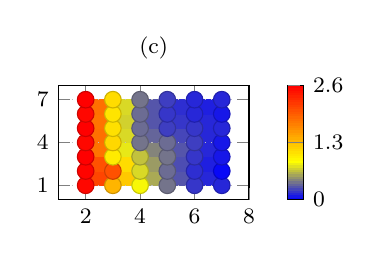
\begin{tikzpicture}
\begin{axis}
[
width=0.33\textwidth,
height=0.25\textwidth,
style={font=\footnotesize},
grid=major,
grid style={dotted},
align=center,
%xlabel={tensor order},
%ylabel={contr. mode (q)},
title={{(c)}}, %  ompfor<qd-slice> ttm<par-loops,seq-blas,$q$-slice>, asymmetric
scaled ticks=false,
zlabel={GFlops},
view={0}{90}, 
ytick={1,4,7,10},
xtick={2,4,6,8},
xmin=1, xmax=8,
ymin=0, ymax=8,
try min ticks=8,
zmin=0, zmax=2600,
point meta min=0, point meta max=2600,
%colormap/jet, 
colormap/hot, 
%colormap/blackwhite,
%colormap={whiteblack}{indices of colormap={\pgfplotscolormaplastindexof{blackwhite},...,0 of blackwhite}},
samples=50,
%colormap access=piecewise const,
colorbar sampled,
colorbar/width=0.2cm,
colorbar style={
point meta min=0, point meta max=2600,
samples=50,
font=\footnotesize,
ytick={0,1300,2600},
yticklabels={0,1.3,2.6},
%title={\scriptsize Gflops},
%ylabel={\scriptsize Gflops},
}
]
%\addplot3[mesh, scatter,samples=50,shader=interp]
%\addplot3[only marks, mesh, scatter,scatter src=z,samples=50,] % z buffer=sort, scatter src=z,
\addplot3[contour filled={number=100},scatter,shader=flat,samples=50]
%\addplot3+[mesh,scatter,shader=flat corner,samples=50, only marks, mark size=2]
coordinates{

(2.000,1.000,2536.639) (2.000,2.000,2549.050) (2.000,3.000,2598.729) (2.000,4.000,2525.744) (2.000,5.000,2590.830) (2.000,6.000,2544.134) (2.000,7.000,2589.762) 

(3.000,1.000,1375.656) (3.000,2.000,2048.636) (3.000,3.000,1013.687) (3.000,4.000,1124.134) (3.000,5.000,1075.977) (3.000,6.000,1052.382) (3.000,7.000,1098.544) 

(4.000,1.000,833.978) (4.000,2.000,732.322) (4.000,3.000,660.833) (4.000,4.000,413.827) (4.000,5.000,368.029) (4.000,6.000,382.244) (4.000,7.000,404.286) 

(5.000,1.000,415.086) (5.000,2.000,368.007) (5.000,3.000,411.465) (5.000,4.000,371.633) (5.000,5.000,212.971) (5.000,6.000,198.100) (5.000,7.000,222.798) 

(6.000,1.000,206.159) (6.000,2.000,156.941) (6.000,3.000,192.783) (6.000,4.000,217.075) (6.000,5.000,186.601) (6.000,6.000,132.454) (6.000,7.000,130.229) 

(7.000,1.000,150.869) (7.000,2.000,27.399) (7.000,3.000,91.695) (7.000,4.000,85.698) (7.000,5.000,132.060) (7.000,6.000,86.740) (7.000,7.000,146.783) 


};
\end{axis}
\end{tikzpicture}

\caption{%
\footnotesize %
Performance maps in double-precision Tflops of the proposed algorithms with varying tensor orders $p$  and contraction modes $q$. 
Tensors are asymmetrically shaped on the top plots and symmetrically shaped on the bottom plots.
In (a) and (d) function \tf{<gemm\_batch>} is executed,
in (b) and (e) \tf{<par-loops,seq-gemm>} with tensor slices, %
in (c) and (f) \tf{<par-loops,seq-gemm>} with subtensors.
\label{performance.tlib.contour}
}
\end{figure*}


\begin{figure*}[t]
\centering
%\tikzset{every mark/.append style={scale=1.5}}
%%%%%%%%%%%%%%%%%%%%%%%%%%%%%%%%%%% Intel MKL Asymmetric (RM+CM)
\begin{tikzpicture}
\begin{axis}[
height=0.2\textheight,
width=0.25\textwidth,
style={font=\footnotesize},
grid=major,
grid style={dotted},
align=center,
%xlabel={Tflops},
ylabel={GFLOPS/core},
ylabel near ticks,
title={(1a)\\\tss{<intel,rm,asymmetric>}}, % intel(mkl) - (ttm<rm>) - asymmetric
title style={yshift=-1.5ex},
ytick={0,10,20,30,40,50},
yticklabels={0,10,20,30,40,50},
ymax=55,
xtick={0,0.25,0.5,0.75,1},
xticklabels={0,25,50,75,100},
mark repeat={16},
cycle list name=compare case 8 for mkl with optimized
]
\addplot %optimized
coordinates{(0.000,9.482) (0.003,9.482) (0.007,10.828) (0.010,10.855) (0.014,10.858) (0.017,11.601) (0.021,11.640) (0.024,12.593) (0.028,13.287) (0.031,20.273) (0.035,20.690) (0.038,21.179) (0.042,21.644) (0.045,22.025) (0.049,22.235) (0.052,23.028) (0.056,23.273) (0.059,23.387) (0.062,23.803) (0.066,23.868) (0.069,23.970) (0.073,24.084) (0.076,24.841) (0.080,25.700) (0.083,26.014) (0.087,26.129) (0.090,26.488) (0.094,26.852) (0.097,27.095) (0.101,27.152) (0.104,27.221) (0.108,27.224) (0.111,27.487) (0.115,27.641) (0.118,27.717) (0.122,28.559) (0.125,28.872) (0.128,29.078) (0.132,29.149) (0.135,29.262) (0.139,29.498) (0.142,29.512) (0.146,29.655) (0.149,29.796) (0.153,29.819) (0.156,29.950) (0.160,29.975) (0.163,29.975) (0.167,30.182) (0.170,30.217) (0.174,30.229) (0.177,30.243) (0.181,30.260) (0.184,30.294) (0.188,30.343) (0.191,30.346) (0.194,30.652) (0.198,30.840) (0.201,30.886) (0.205,30.898) (0.208,30.910) (0.212,30.956) (0.215,31.053) (0.219,31.175) (0.222,31.258) (0.226,31.326) (0.229,31.341) (0.233,31.347) (0.236,31.365) (0.240,31.408) (0.243,31.483) (0.247,31.493) (0.250,31.509) (0.253,31.657) (0.257,31.669) (0.260,31.915) (0.264,32.093) (0.267,32.100) (0.271,32.142) (0.274,32.212) (0.278,32.345) (0.281,32.490) (0.285,32.567) (0.288,32.666) (0.292,32.732) (0.295,32.735) (0.299,32.805) (0.302,32.816) (0.306,32.875) (0.309,32.879) (0.312,33.027) (0.316,33.073) (0.319,33.122) (0.323,33.176) (0.326,33.292) (0.330,33.299) (0.333,33.599) (0.337,33.679) (0.340,33.765) (0.344,33.818) (0.347,33.956) (0.351,33.959) (0.354,33.994) (0.358,34.037) (0.361,34.053) (0.365,34.170) (0.368,34.204) (0.372,34.274) (0.375,34.336) (0.378,34.435) (0.382,34.518) (0.385,34.573) (0.389,34.590) (0.392,34.646) (0.396,34.663) (0.399,34.688) (0.403,34.964) (0.406,34.986) (0.410,34.994) (0.413,35.024) (0.417,35.106) (0.420,35.126) (0.424,35.142) (0.427,35.147) (0.431,35.172) (0.434,35.174) (0.438,35.204) (0.441,35.251) (0.444,35.329) (0.448,35.342) (0.451,35.482) (0.455,35.501) (0.458,35.564) (0.462,35.567) (0.465,35.572) (0.469,35.589) (0.472,35.669) (0.476,35.672) (0.479,35.914) (0.483,35.956) (0.486,35.986) (0.490,35.993) (0.493,36.041) (0.497,36.083) (0.500,36.146) (0.503,36.158) (0.507,36.180) (0.510,36.187) (0.514,36.243) (0.517,36.273) (0.521,36.300) (0.524,36.333) (0.528,36.340) (0.531,36.488) (0.535,36.636) (0.538,36.701) (0.542,36.740) (0.545,36.764) (0.549,36.779) (0.552,36.782) (0.556,36.801) (0.559,36.885) (0.562,36.897) (0.566,36.933) (0.569,36.934) (0.573,36.952) (0.576,37.042) (0.580,37.216) (0.583,37.230) (0.587,37.244) (0.590,37.383) (0.594,37.521) (0.597,37.687) (0.601,37.702) (0.604,37.747) (0.608,37.913) (0.611,37.930) (0.615,38.007) (0.618,38.076) (0.622,38.114) (0.625,38.229) (0.628,38.255) (0.632,38.435) (0.635,38.531) (0.639,38.660) (0.642,38.713) (0.646,38.806) (0.649,38.856) (0.653,38.891) (0.656,38.893) (0.660,38.927) (0.663,38.949) (0.667,38.950) (0.670,39.067) (0.674,39.091) (0.677,39.111) (0.681,39.162) (0.684,39.209) (0.688,39.241) (0.691,39.296) (0.694,39.456) (0.698,39.482) (0.701,39.484) (0.705,39.857) (0.708,39.874) (0.712,40.084) (0.715,40.136) (0.719,40.162) (0.722,40.166) (0.726,40.210) (0.729,40.298) (0.733,40.369) (0.736,40.402) (0.740,40.421) (0.743,40.432) (0.747,40.436) (0.750,40.451) (0.753,40.491) (0.757,40.548) (0.760,40.562) (0.764,40.601) (0.767,40.703) (0.771,40.815) (0.774,40.853) (0.778,40.893) (0.781,40.961) (0.785,40.999) (0.788,41.082) (0.792,41.147) (0.795,41.155) (0.799,41.194) (0.802,41.242) (0.806,41.252) (0.809,41.430) (0.812,41.456) (0.816,41.480) (0.819,41.500) (0.823,41.570) (0.826,41.591) (0.830,41.656) (0.833,41.891) (0.837,41.982) (0.840,42.072) (0.844,42.142) (0.847,42.166) (0.851,42.192) (0.854,42.208) (0.858,42.250) (0.861,42.340) (0.865,42.360) (0.868,42.371) (0.872,42.372) (0.875,42.377) (0.878,42.381) (0.882,42.460) (0.885,42.684) (0.889,42.690) (0.892,42.795) (0.896,42.930) (0.899,42.931) (0.903,43.104) (0.906,43.191) (0.910,43.310) (0.913,43.329) (0.917,43.440) (0.920,43.441) (0.924,43.509) (0.927,43.510) (0.931,43.531) (0.934,43.651) (0.938,43.683) (0.941,43.738) (0.944,43.798) (0.948,43.816) (0.951,43.836) (0.955,43.876) (0.958,44.213) (0.962,44.344) (0.965,44.470) (0.969,44.519) (0.972,44.820) (0.976,44.911) (0.979,45.121) (0.983,46.385) (0.986,46.440) (0.990,46.663) (0.993,46.848) (0.997,46.921) (1.000,46.966) };
\addplot
coordinates{(0.0,5.816) (0.004,5.816) (0.009,6.07) (0.013,6.486) (0.018,6.675) (0.022,6.847) (0.027,6.88) (0.031,6.954) (0.036,7.01) (0.04,9.553) (0.045,10.444) (0.049,10.895) (0.054,11.358) (0.058,11.4) (0.062,11.431) (0.067,11.441) (0.071,11.482) (0.076,11.504) (0.08,11.674) (0.085,11.774) (0.089,11.976) (0.094,12.152) (0.098,12.369) (0.103,12.413) (0.107,12.442) (0.112,12.507) (0.116,12.641) (0.121,12.731) (0.125,12.743) (0.129,12.817) (0.134,13.147) (0.138,13.278) (0.143,20.152) (0.147,20.257) (0.152,20.918) (0.156,20.962) (0.161,21.228) (0.165,21.262) (0.17,21.379) (0.174,21.526) (0.179,21.65) (0.183,21.666) (0.188,21.754) (0.192,21.807) (0.196,21.835) (0.201,21.903) (0.205,21.917) (0.21,21.977) (0.214,22.015) (0.219,22.043) (0.223,22.123) (0.228,22.155) (0.232,22.195) (0.237,22.206) (0.241,22.319) (0.246,22.472) (0.25,22.542) (0.254,22.547) (0.259,22.83) (0.263,22.945) (0.268,23.7) (0.272,24.124) (0.277,24.171) (0.281,24.212) (0.286,25.844) (0.29,25.889) (0.295,26.185) (0.299,26.534) (0.304,26.699) (0.308,26.913) (0.312,27.014) (0.317,27.266) (0.321,27.638) (0.326,28.182) (0.33,28.885) (0.335,29.163) (0.339,29.76) (0.344,29.847) (0.348,30.074) (0.353,30.208) (0.357,30.314) (0.362,30.541) (0.366,30.601) (0.371,30.609) (0.375,30.74) (0.379,30.959) (0.384,31.105) (0.388,31.133) (0.393,31.202) (0.397,31.262) (0.402,31.366) (0.406,31.726) (0.411,31.77) (0.415,32.018) (0.42,32.149) (0.424,32.286) (0.429,32.618) (0.433,32.649) (0.437,32.695) (0.442,32.736) (0.446,32.968) (0.451,33.04) (0.455,33.153) (0.46,33.211) (0.464,33.362) (0.469,33.487) (0.473,33.575) (0.478,33.719) (0.482,33.731) (0.487,33.81) (0.491,33.848) (0.496,33.899) (0.5,34.084) (0.504,34.088) (0.509,34.102) (0.513,34.106) (0.518,34.127) (0.522,34.172) (0.527,34.225) (0.531,34.276) (0.536,34.283) (0.54,34.403) (0.545,34.488) (0.549,34.493) (0.554,34.537) (0.558,34.743) (0.562,34.999) (0.567,35.095) (0.571,35.102) (0.576,35.195) (0.58,35.355) (0.585,35.366) (0.589,35.593) (0.594,35.604) (0.598,35.648) (0.603,35.79) (0.607,35.854) (0.612,35.891) (0.616,35.907) (0.621,35.947) (0.625,35.978) (0.629,36.068) (0.634,36.084) (0.638,36.112) (0.643,36.135) (0.647,36.289) (0.652,36.353) (0.656,36.388) (0.661,36.473) (0.665,36.479) (0.67,36.521) (0.674,36.589) (0.679,36.617) (0.683,36.637) (0.688,36.735) (0.692,36.737) (0.696,36.765) (0.701,36.871) (0.705,36.965) (0.71,36.997) (0.714,37.009) (0.719,37.033) (0.723,37.062) (0.728,37.063) (0.732,37.132) (0.737,37.135) (0.741,37.152) (0.746,37.16) (0.75,37.186) (0.754,37.292) (0.759,37.312) (0.763,37.332) (0.768,37.34) (0.772,37.366) (0.777,37.406) (0.781,37.485) (0.786,37.519) (0.79,37.533) (0.795,37.549) (0.799,37.599) (0.804,37.655) (0.808,37.662) (0.812,37.72) (0.817,37.741) (0.821,37.867) (0.826,37.935) (0.83,37.983) (0.835,38.076) (0.839,38.265) (0.844,38.34) (0.848,38.584) (0.853,38.631) (0.857,38.69) (0.862,38.789) (0.866,38.838) (0.871,38.911) (0.875,38.95) (0.879,39.106) (0.884,39.255) (0.888,39.443) (0.893,39.736) (0.897,39.922) (0.902,40.301) (0.906,40.342) (0.911,40.389) (0.915,40.462) (0.92,40.551) (0.924,41.137) (0.929,41.224) (0.933,41.47) (0.938,41.636) (0.942,41.801) (0.946,41.975) (0.951,42.286) (0.955,42.568) (0.96,42.634) (0.964,42.683) (0.969,43.803) (0.973,44.109) (0.978,44.471) (0.982,44.58) (0.987,45.009) (0.991,45.114) (0.996,45.193) (1.0,45.959) };
\addplot
coordinates{(0.0,2.134) (0.004,2.134) (0.009,3.524) (0.013,3.543) (0.018,3.997) (0.022,4.586) (0.027,4.804) (0.031,5.079) (0.036,5.133) (0.04,5.218) (0.045,5.249) (0.049,5.304) (0.054,5.578) (0.058,5.591) (0.062,5.627) (0.067,5.675) (0.071,5.692) (0.076,5.794) (0.08,5.804) (0.085,5.861) (0.089,5.862) (0.094,5.892) (0.098,5.895) (0.103,5.908) (0.107,5.964) (0.112,6.006) (0.116,6.03) (0.121,6.047) (0.125,6.096) (0.129,6.1) (0.134,6.186) (0.138,6.189) (0.143,6.225) (0.147,6.232) (0.152,6.257) (0.156,6.301) (0.161,6.334) (0.165,6.387) (0.17,6.436) (0.174,6.442) (0.179,6.457) (0.183,6.464) (0.188,6.546) (0.192,6.58) (0.196,6.609) (0.201,6.635) (0.205,6.698) (0.21,6.729) (0.214,6.751) (0.219,6.758) (0.223,6.815) (0.228,6.903) (0.232,6.918) (0.237,6.922) (0.241,6.935) (0.246,6.943) (0.25,6.957) (0.254,6.967) (0.259,6.973) (0.263,7.012) (0.268,7.126) (0.272,8.041) (0.277,9.403) (0.281,9.484) (0.286,9.921) (0.29,9.928) (0.295,10.081) (0.299,10.25) (0.304,10.304) (0.308,10.398) (0.312,10.401) (0.317,10.702) (0.321,10.786) (0.326,10.901) (0.33,10.925) (0.335,11.011) (0.339,11.014) (0.344,11.071) (0.348,11.126) (0.353,11.187) (0.357,11.275) (0.362,11.293) (0.366,11.304) (0.371,11.338) (0.375,11.343) (0.379,11.463) (0.384,11.506) (0.388,11.534) (0.393,11.563) (0.397,11.753) (0.402,11.842) (0.406,11.848) (0.411,11.899) (0.415,11.991) (0.42,12.098) (0.424,12.173) (0.429,12.194) (0.433,12.335) (0.437,12.361) (0.442,12.384) (0.446,12.487) (0.451,12.53) (0.455,12.707) (0.46,12.759) (0.464,12.79) (0.469,12.869) (0.473,12.879) (0.478,13.012) (0.482,13.126) (0.487,13.155) (0.491,13.662) (0.496,15.186) (0.5,16.498) (0.504,16.518) (0.509,17.083) (0.513,17.32) (0.518,17.748) (0.522,18.234) (0.527,18.869) (0.531,19.263) (0.536,19.538) (0.54,19.649) (0.545,19.741) (0.549,19.796) (0.554,20.126) (0.558,20.594) (0.562,20.757) (0.567,20.897) (0.571,21.095) (0.576,21.163) (0.58,21.21) (0.585,21.291) (0.589,21.556) (0.594,21.627) (0.598,21.845) (0.603,21.856) (0.607,21.952) (0.612,22.037) (0.616,22.073) (0.621,22.075) (0.625,22.08) (0.629,22.1) (0.634,22.191) (0.638,22.311) (0.643,22.327) (0.647,22.346) (0.652,22.375) (0.656,22.375) (0.661,22.429) (0.665,22.504) (0.67,22.864) (0.674,23.122) (0.679,23.186) (0.683,23.194) (0.688,25.378) (0.692,25.735) (0.696,27.146) (0.701,27.611) (0.705,27.871) (0.71,29.217) (0.714,29.457) (0.719,29.966) (0.723,30.031) (0.728,30.039) (0.732,30.704) (0.737,30.862) (0.741,31.382) (0.746,31.447) (0.75,31.756) (0.754,31.855) (0.759,31.935) (0.763,32.384) (0.768,32.515) (0.772,32.647) (0.777,32.806) (0.781,33.009) (0.786,33.272) (0.79,33.548) (0.795,33.995) (0.799,34.31) (0.804,34.579) (0.808,34.609) (0.812,35.279) (0.817,35.535) (0.821,35.573) (0.826,35.935) (0.83,35.971) (0.835,35.986) (0.839,36.003) (0.844,36.195) (0.848,36.348) (0.853,36.622) (0.857,36.637) (0.862,36.658) (0.866,36.843) (0.871,36.994) (0.875,37.091) (0.879,37.191) (0.884,37.236) (0.888,37.261) (0.893,37.266) (0.897,37.358) (0.902,37.4) (0.906,37.493) (0.911,37.542) (0.915,37.578) (0.92,37.733) (0.924,37.82) (0.929,38.078) (0.933,38.431) (0.938,38.788) (0.942,38.965) (0.946,39.155) (0.951,40.914) (0.955,40.922) (0.96,42.219) (0.964,42.793) (0.969,43.205) (0.973,43.765) (0.978,44.121) (0.982,44.25) (0.987,44.397) (0.991,44.704) (0.996,46.249) (1.0,47.123) };
\addplot
coordinates{(0.0,9.12) (0.004,9.12) (0.009,9.592) (0.013,10.579) (0.018,11.189) (0.022,11.423) (0.027,11.544) (0.031,12.133) (0.036,15.128) (0.04,15.385) (0.045,17.789) (0.049,18.157) (0.054,18.949) (0.058,18.974) (0.062,19.131) (0.067,20.398) (0.071,20.457) (0.076,20.723) (0.08,20.812) (0.085,21.294) (0.089,21.691) (0.094,21.771) (0.098,22.019) (0.103,22.435) (0.107,22.806) (0.112,22.864) (0.116,23.188) (0.121,23.484) (0.125,23.679) (0.129,23.729) (0.134,23.786) (0.138,23.792) (0.143,23.956) (0.147,23.98) (0.152,24.179) (0.156,24.307) (0.161,24.332) (0.165,24.561) (0.17,24.908) (0.174,25.027) (0.179,25.428) (0.183,25.872) (0.188,25.971) (0.192,26.144) (0.196,26.236) (0.201,26.266) (0.205,26.554) (0.21,26.995) (0.214,27.014) (0.219,27.772) (0.223,28.384) (0.228,28.412) (0.232,28.554) (0.237,29.001) (0.241,29.012) (0.246,29.17) (0.25,29.217) (0.254,29.494) (0.259,29.635) (0.263,29.639) (0.268,29.731) (0.272,29.762) (0.277,29.885) (0.281,29.94) (0.286,30.038) (0.29,30.106) (0.295,30.141) (0.299,30.175) (0.304,30.323) (0.308,30.421) (0.312,31.045) (0.317,31.444) (0.321,31.542) (0.326,31.644) (0.33,31.705) (0.335,31.766) (0.339,31.852) (0.344,32.065) (0.348,32.177) (0.353,32.533) (0.357,32.658) (0.362,32.718) (0.366,33.29) (0.371,33.615) (0.375,33.7) (0.379,33.853) (0.384,33.885) (0.388,33.938) (0.393,33.95) (0.397,33.958) (0.402,34.064) (0.406,34.197) (0.411,34.263) (0.415,34.414) (0.42,34.726) (0.424,34.773) (0.429,34.829) (0.433,34.868) (0.437,34.995) (0.442,35.053) (0.446,35.086) (0.451,35.164) (0.455,35.166) (0.46,35.264) (0.464,35.268) (0.469,35.338) (0.473,35.529) (0.478,35.838) (0.482,35.953) (0.487,36.242) (0.491,36.578) (0.496,36.59) (0.5,36.637) (0.504,36.82) (0.509,36.875) (0.513,36.98) (0.518,36.986) (0.522,37.1) (0.527,37.396) (0.531,37.622) (0.536,37.683) (0.54,37.774) (0.545,37.786) (0.549,37.792) (0.554,37.926) (0.558,37.94) (0.562,37.942) (0.567,37.991) (0.571,38.058) (0.576,38.086) (0.58,38.126) (0.585,38.208) (0.589,38.239) (0.594,38.24) (0.598,38.537) (0.603,38.547) (0.607,38.575) (0.612,38.602) (0.616,38.687) (0.621,38.969) (0.625,38.987) (0.629,39.026) (0.634,39.089) (0.638,39.092) (0.643,39.132) (0.647,39.158) (0.652,39.158) (0.656,39.186) (0.661,39.266) (0.665,39.317) (0.67,39.322) (0.674,39.346) (0.679,39.367) (0.683,39.37) (0.688,39.435) (0.692,39.44) (0.696,39.459) (0.701,39.51) (0.705,39.567) (0.71,39.58) (0.714,39.597) (0.719,39.636) (0.723,39.679) (0.728,39.685) (0.732,39.7) (0.737,39.719) (0.741,39.722) (0.746,39.743) (0.75,39.767) (0.754,39.782) (0.759,39.888) (0.763,39.967) (0.768,40.01) (0.772,40.043) (0.777,40.064) (0.781,40.1) (0.786,40.111) (0.79,40.111) (0.795,40.185) (0.799,40.235) (0.804,40.274) (0.808,40.403) (0.812,40.422) (0.817,40.464) (0.821,40.468) (0.826,40.514) (0.83,40.516) (0.835,40.573) (0.839,40.617) (0.844,40.76) (0.848,40.762) (0.853,40.78) (0.857,40.796) (0.862,40.799) (0.866,40.851) (0.871,40.854) (0.875,40.936) (0.879,40.989) (0.884,41.028) (0.888,41.089) (0.893,41.135) (0.897,41.185) (0.902,41.308) (0.906,41.334) (0.911,41.433) (0.915,41.507) (0.92,41.523) (0.924,41.526) (0.929,41.692) (0.933,41.777) (0.938,41.782) (0.942,41.92) (0.946,41.921) (0.951,42.024) (0.955,42.08) (0.96,42.101) (0.964,42.167) (0.969,42.27) (0.973,42.702) (0.978,42.729) (0.982,42.802) (0.987,42.947) (0.991,43.006) (0.996,43.332) (1.0,43.425)};
\addplot
coordinates{(0.0,6.738) (0.004,6.738) (0.009,6.877) (0.013,7.535) (0.018,7.677) (0.022,9.119) (0.027,10.632) (0.031,11.127) (0.036,13.266) (0.04,13.406) (0.045,13.486) (0.049,13.885) (0.054,13.978) (0.058,14.249) (0.062,14.316) (0.067,16.187) (0.071,16.494) (0.076,18.467) (0.08,18.94) (0.085,19.284) (0.089,19.925) (0.094,20.281) (0.098,20.61) (0.103,20.669) (0.107,20.718) (0.112,20.771) (0.116,21.142) (0.121,21.271) (0.125,21.626) (0.129,21.699) (0.134,21.957) (0.138,22.069) (0.143,22.122) (0.147,22.271) (0.152,22.579) (0.156,22.625) (0.161,22.862) (0.165,22.955) (0.17,23.106) (0.174,23.155) (0.179,23.187) (0.183,23.255) (0.188,23.501) (0.192,23.77) (0.196,23.949) (0.201,23.95) (0.205,24.048) (0.21,24.07) (0.214,24.092) (0.219,24.34) (0.223,24.619) (0.228,24.738) (0.232,24.746) (0.237,24.92) (0.241,25.199) (0.246,25.323) (0.25,25.377) (0.254,25.435) (0.259,25.438) (0.263,25.795) (0.268,25.972) (0.272,26.396) (0.277,26.591) (0.281,26.649) (0.286,26.702) (0.29,26.717) (0.295,27.063) (0.299,28.029) (0.304,28.074) (0.308,28.112) (0.312,28.371) (0.317,28.606) (0.321,28.622) (0.326,28.923) (0.33,29.104) (0.335,29.125) (0.339,29.175) (0.344,29.345) (0.348,29.53) (0.353,29.934) (0.357,30.383) (0.362,30.598) (0.366,30.625) (0.371,30.805) (0.375,30.93) (0.379,30.969) (0.384,31.033) (0.388,31.088) (0.393,31.194) (0.397,31.323) (0.402,31.473) (0.406,31.672) (0.411,31.702) (0.415,31.714) (0.42,31.79) (0.424,31.842) (0.429,31.89) (0.433,32.128) (0.437,32.53) (0.442,32.834) (0.446,32.943) (0.451,32.971) (0.455,33.065) (0.46,33.164) (0.464,33.325) (0.469,33.464) (0.473,33.495) (0.478,33.662) (0.482,33.79) (0.487,33.816) (0.491,33.958) (0.496,34.043) (0.5,34.152) (0.504,34.19) (0.509,34.817) (0.513,34.87) (0.518,35.109) (0.522,35.223) (0.527,35.33) (0.531,35.336) (0.536,35.38) (0.54,35.628) (0.545,35.669) (0.549,35.885) (0.554,35.893) (0.558,36.019) (0.562,36.042) (0.567,36.134) (0.571,36.171) (0.576,36.271) (0.58,36.335) (0.585,36.38) (0.589,36.668) (0.594,36.74) (0.598,36.806) (0.603,36.838) (0.607,37.178) (0.612,37.216) (0.616,37.244) (0.621,37.27) (0.625,37.295) (0.629,37.313) (0.634,37.396) (0.638,37.543) (0.643,37.589) (0.647,37.641) (0.652,37.67) (0.656,37.68) (0.661,37.702) (0.665,37.724) (0.67,37.731) (0.674,37.775) (0.679,37.798) (0.683,37.917) (0.688,38.017) (0.692,38.04) (0.696,38.048) (0.701,38.065) (0.705,38.08) (0.71,38.13) (0.714,38.235) (0.719,38.276) (0.723,38.308) (0.728,38.32) (0.732,38.323) (0.737,38.411) (0.741,38.463) (0.746,38.474) (0.75,38.498) (0.754,38.522) (0.759,38.549) (0.763,38.554) (0.768,38.582) (0.772,38.733) (0.777,38.751) (0.781,38.77) (0.786,38.779) (0.79,38.813) (0.795,38.834) (0.799,38.858) (0.804,38.892) (0.808,38.932) (0.812,39.004) (0.817,39.151) (0.821,39.187) (0.826,39.286) (0.83,39.305) (0.835,39.339) (0.839,39.348) (0.844,39.365) (0.848,39.419) (0.853,39.423) (0.857,39.45) (0.862,39.518) (0.866,39.527) (0.871,39.587) (0.875,39.605) (0.879,39.625) (0.884,39.65) (0.888,39.664) (0.893,39.755) (0.897,39.799) (0.902,39.85) (0.906,39.86) (0.911,39.904) (0.915,39.945) (0.92,39.955) (0.924,39.996) (0.929,40.02) (0.933,40.03) (0.938,40.137) (0.942,40.216) (0.946,40.261) (0.951,40.283) (0.955,40.435) (0.96,40.611) (0.964,40.835) (0.969,41.639) (0.973,41.913) (0.978,41.971) (0.982,42.414) (0.987,42.838) (0.991,42.918) (0.996,43.353) (1.0,43.728) };
\addplot
coordinates{(0.0,4.928) (0.004,4.928) (0.009,5.104) (0.013,5.273) (0.018,5.851) (0.022,6.134) (0.027,6.196) (0.031,6.416) (0.036,6.686) (0.04,6.985) (0.045,7.276) (0.049,7.425) (0.054,7.54) (0.058,7.622) (0.062,7.65) (0.067,7.7) (0.071,7.708) (0.076,7.812) (0.08,7.9) (0.085,7.961) (0.089,7.982) (0.094,8.089) (0.098,8.427) (0.103,8.428) (0.107,8.48) (0.112,8.592) (0.116,8.625) (0.121,8.751) (0.125,8.874) (0.129,8.997) (0.134,9.021) (0.138,9.033) (0.143,9.068) (0.147,9.134) (0.152,9.159) (0.156,9.236) (0.161,9.237) (0.165,9.253) (0.17,9.331) (0.174,9.488) (0.179,9.514) (0.183,9.538) (0.188,9.61) (0.192,9.713) (0.196,9.741) (0.201,9.777) (0.205,9.838) (0.21,9.874) (0.214,10.079) (0.219,10.083) (0.223,10.088) (0.228,10.141) (0.232,10.188) (0.237,10.274) (0.241,10.283) (0.246,10.319) (0.25,10.457) (0.254,10.491) (0.259,10.547) (0.263,10.605) (0.268,10.635) (0.272,10.64) (0.277,10.671) (0.281,10.684) (0.286,10.745) (0.29,10.751) (0.295,10.787) (0.299,10.799) (0.304,10.808) (0.308,10.873) (0.312,10.913) (0.317,10.976) (0.321,10.995) (0.326,11.059) (0.33,11.064) (0.335,11.08) (0.339,11.109) (0.344,11.176) (0.348,11.182) (0.353,11.192) (0.357,11.201) (0.362,11.203) (0.366,11.272) (0.371,11.301) (0.375,11.333) (0.379,11.394) (0.384,11.398) (0.388,11.409) (0.393,11.411) (0.397,11.417) (0.402,11.455) (0.406,11.458) (0.411,11.458) (0.415,11.46) (0.42,11.465) (0.424,11.477) (0.429,11.487) (0.433,11.556) (0.437,11.575) (0.442,11.6) (0.446,11.678) (0.451,11.698) (0.455,11.703) (0.46,11.717) (0.464,11.766) (0.469,11.86) (0.473,11.877) (0.478,11.938) (0.482,11.958) (0.487,12.378) (0.491,12.434) (0.496,12.487) (0.5,12.52) (0.504,12.781) (0.509,12.797) (0.513,12.88) (0.518,13.044) (0.522,13.195) (0.527,13.346) (0.531,13.349) (0.536,13.516) (0.54,13.604) (0.545,13.68) (0.549,13.837) (0.554,14.335) (0.558,15.331) (0.562,15.395) (0.567,15.4) (0.571,15.498) (0.576,15.884) (0.58,15.912) (0.585,15.92) (0.589,15.945) (0.594,16.717) (0.598,17.51) (0.603,18.044) (0.607,19.616) (0.612,19.817) (0.616,20.629) (0.621,21.023) (0.625,21.95) (0.629,24.284) (0.634,24.944) (0.638,24.975) (0.643,25.85) (0.647,26.123) (0.652,26.549) (0.656,26.566) (0.661,26.832) (0.665,26.915) (0.67,26.966) (0.674,27.46) (0.679,27.723) (0.683,27.793) (0.688,28.101) (0.692,28.508) (0.696,28.875) (0.701,28.876) (0.705,28.932) (0.71,29.14) (0.714,29.405) (0.719,29.615) (0.723,29.689) (0.728,29.79) (0.732,29.964) (0.737,30.003) (0.741,30.124) (0.746,30.272) (0.75,30.391) (0.754,30.41) (0.759,30.645) (0.763,30.652) (0.768,30.847) (0.772,31.163) (0.777,31.233) (0.781,31.809) (0.786,31.862) (0.79,32.254) (0.795,32.283) (0.799,32.428) (0.804,32.807) (0.808,32.807) (0.812,32.808) (0.817,32.919) (0.821,32.992) (0.826,33.275) (0.83,33.357) (0.835,33.359) (0.839,33.582) (0.844,33.601) (0.848,33.677) (0.853,33.728) (0.857,33.851) (0.862,34.047) (0.866,34.332) (0.871,34.397) (0.875,34.44) (0.879,34.916) (0.884,35.287) (0.888,35.322) (0.893,35.348) (0.897,35.365) (0.902,35.417) (0.906,35.555) (0.911,35.868) (0.915,36.086) (0.92,36.251) (0.924,36.761) (0.929,36.829) (0.933,37.438) (0.938,37.449) (0.942,37.463) (0.946,37.696) (0.951,38.119) (0.955,38.236) (0.96,38.902) (0.964,38.957) (0.969,39.286) (0.973,39.593) (0.978,39.661) (0.982,39.984) (0.987,40.229) (0.991,40.337) (0.996,42.242) (1.0,42.78)};
\end{axis}
\end{tikzpicture}
\hfill
\begin{tikzpicture}
\begin{axis}[
height=0.2\textheight,
width=0.25\textwidth,
style={font=\footnotesize},
grid=major,
grid style={dotted},
align=center,
%xlabel={Tflops},
%ylabel={Cumulative Probability},
%ylabel near ticks,
title={(1b)\\\tss{<intel,cm,asymmetric>}}, % intel(mkl) - (ttm<cm>) - asymmetric
title style={yshift=-1.5ex},
ytick={0,10,20,30,40,50},
yticklabels={0,10,20,30,40,50},
ymax=55,
xtick={0,0.25,0.5,0.75,1},
xticklabels={0,25,50,75,100},
mark repeat={4},
cycle list name=compare case 8 for mkl with optimized
]
\addplot
coordinates{(0.000,9.389) (0.003,9.389) (0.007,10.664) (0.010,11.198) (0.014,11.503) (0.017,11.776) (0.021,12.442) (0.024,12.740) (0.028,13.509) (0.031,19.710) (0.035,19.785) (0.038,20.201) (0.042,21.218) (0.045,21.872) (0.049,22.083) (0.052,22.165) (0.056,22.165) (0.059,22.242) (0.062,23.409) (0.066,23.634) (0.069,24.058) (0.073,25.114) (0.076,25.211) (0.080,26.154) (0.083,26.252) (0.087,26.344) (0.090,27.033) (0.094,27.333) (0.097,27.629) (0.101,27.933) (0.104,27.977) (0.108,27.998) (0.111,28.185) (0.115,28.397) (0.118,28.418) (0.122,28.454) (0.125,28.490) (0.128,28.610) (0.132,28.682) (0.135,28.847) (0.139,28.861) (0.142,29.007) (0.146,29.150) (0.149,29.537) (0.153,29.654) (0.156,29.698) (0.160,29.784) (0.163,29.846) (0.167,29.882) (0.170,29.897) (0.174,29.900) (0.177,29.905) (0.181,30.034) (0.184,30.145) (0.188,30.146) (0.191,30.169) (0.194,30.294) (0.198,30.505) (0.201,30.512) (0.205,30.527) (0.208,30.546) (0.212,30.579) (0.215,30.600) (0.219,30.665) (0.222,30.760) (0.226,30.794) (0.229,30.964) (0.233,30.992) (0.236,31.062) (0.240,31.087) (0.243,31.172) (0.247,31.304) (0.250,31.320) (0.253,31.478) (0.257,31.589) (0.260,31.627) (0.264,31.714) (0.267,31.930) (0.271,32.000) (0.274,32.004) (0.278,32.121) (0.281,32.174) (0.285,32.238) (0.288,32.303) (0.292,32.325) (0.295,32.366) (0.299,32.415) (0.302,32.663) (0.306,32.752) (0.309,32.847) (0.312,32.851) (0.316,32.886) (0.319,33.031) (0.323,33.042) (0.326,33.424) (0.330,33.546) (0.333,33.567) (0.337,33.573) (0.340,33.578) (0.344,33.597) (0.347,33.646) (0.351,33.683) (0.354,33.718) (0.358,33.767) (0.361,33.770) (0.365,33.787) (0.368,33.854) (0.372,33.938) (0.375,33.962) (0.378,34.142) (0.382,34.247) (0.385,34.310) (0.389,34.311) (0.392,34.366) (0.396,34.396) (0.399,34.405) (0.403,34.570) (0.406,34.646) (0.410,34.662) (0.413,34.712) (0.417,34.821) (0.420,34.980) (0.424,35.008) (0.427,35.010) (0.431,35.051) (0.434,35.088) (0.438,35.111) (0.441,35.129) (0.444,35.252) (0.448,35.269) (0.451,35.313) (0.455,35.372) (0.458,35.419) (0.462,35.425) (0.465,35.473) (0.469,35.523) (0.472,35.534) (0.476,35.611) (0.479,35.647) (0.483,35.649) (0.486,35.687) (0.490,35.832) (0.493,35.847) (0.497,35.914) (0.500,35.943) (0.503,35.988) (0.507,36.130) (0.510,36.301) (0.514,36.325) (0.517,36.332) (0.521,36.346) (0.524,36.357) (0.528,36.415) (0.531,36.485) (0.535,36.485) (0.538,36.524) (0.542,36.532) (0.545,36.560) (0.549,36.569) (0.552,36.631) (0.556,36.687) (0.559,36.898) (0.562,36.908) (0.566,36.942) (0.569,36.953) (0.573,36.993) (0.576,37.062) (0.580,37.063) (0.583,37.127) (0.587,37.140) (0.590,37.146) (0.594,37.148) (0.597,37.149) (0.601,37.240) (0.604,37.272) (0.608,37.302) (0.611,37.347) (0.615,37.357) (0.618,37.594) (0.622,37.629) (0.625,37.704) (0.628,37.714) (0.632,37.863) (0.635,37.962) (0.639,37.991) (0.642,38.002) (0.646,38.015) (0.649,38.044) (0.653,38.122) (0.656,38.141) (0.660,38.233) (0.663,38.257) (0.667,38.301) (0.670,38.350) (0.674,38.375) (0.677,38.419) (0.681,38.439) (0.684,38.475) (0.688,38.519) (0.691,38.550) (0.694,38.567) (0.698,38.578) (0.701,38.620) (0.705,38.857) (0.708,38.953) (0.712,39.289) (0.715,39.479) (0.719,39.540) (0.722,39.588) (0.726,39.744) (0.729,39.806) (0.733,39.807) (0.736,40.039) (0.740,40.105) (0.743,40.192) (0.747,40.327) (0.750,40.346) (0.753,40.418) (0.757,40.424) (0.760,40.579) (0.764,40.590) (0.767,40.602) (0.771,40.666) (0.774,40.811) (0.778,40.946) (0.781,40.951) (0.785,40.956) (0.788,40.962) (0.792,41.032) (0.795,41.040) (0.799,41.077) (0.802,41.110) (0.806,41.132) (0.809,41.137) (0.812,41.138) (0.816,41.161) (0.819,41.183) (0.823,41.224) (0.826,41.242) (0.830,41.259) (0.833,41.295) (0.837,41.333) (0.840,41.360) (0.844,41.376) (0.847,41.389) (0.851,41.439) (0.854,41.460) (0.858,41.654) (0.861,41.658) (0.865,41.805) (0.868,41.834) (0.872,41.875) (0.875,41.882) (0.878,41.972) (0.882,42.173) (0.885,42.212) (0.889,42.274) (0.892,42.279) (0.896,42.308) (0.899,42.412) (0.903,42.451) (0.906,42.458) (0.910,42.553) (0.913,42.601) (0.917,42.725) (0.920,42.726) (0.924,42.866) (0.927,42.917) (0.931,43.030) (0.934,43.071) (0.938,43.191) (0.941,43.305) (0.944,43.375) (0.948,43.557) (0.951,43.728) (0.955,43.733) (0.958,43.790) (0.962,43.863) (0.965,44.014) (0.969,44.024) (0.972,44.080) (0.976,44.156) (0.979,44.320) (0.983,44.322) (0.986,44.339) (0.990,44.891) (0.993,45.544) (0.997,46.045) (1.000,47.045) };
\addplot
coordinates{(0.000,5.678) (0.004,5.678) (0.009,5.929) (0.013,6.283) (0.018,6.465) (0.022,6.598) (0.027,6.680) (0.031,6.757) (0.036,6.801) (0.040,10.459) (0.045,10.592) (0.049,10.908) (0.054,11.048) (0.058,11.112) (0.062,11.121) (0.067,11.136) (0.071,11.183) (0.076,11.186) (0.080,11.495) (0.085,11.596) (0.089,11.609) (0.094,11.898) (0.098,12.018) (0.103,12.170) (0.107,12.463) (0.112,12.500) (0.116,12.516) (0.121,12.560) (0.125,12.606) (0.129,12.627) (0.134,12.843) (0.138,13.395) (0.143,19.905) (0.147,20.121) (0.152,20.933) (0.156,21.117) (0.161,21.198) (0.165,21.199) (0.170,21.224) (0.174,21.227) (0.179,21.314) (0.183,21.374) (0.188,21.380) (0.192,21.399) (0.196,21.447) (0.201,21.468) (0.205,21.538) (0.210,21.557) (0.214,21.839) (0.219,21.842) (0.223,21.877) (0.228,21.885) (0.232,21.929) (0.237,21.992) (0.241,22.046) (0.246,22.095) (0.250,22.139) (0.254,22.191) (0.259,22.262) (0.263,22.280) (0.268,22.365) (0.272,22.448) (0.277,22.532) (0.281,22.781) (0.286,22.970) (0.290,23.603) (0.295,24.135) (0.299,25.107) (0.304,25.327) (0.308,25.673) (0.312,26.132) (0.317,26.231) (0.321,27.233) (0.326,27.235) (0.330,27.642) (0.335,27.733) (0.339,27.849) (0.344,27.934) (0.348,28.375) (0.353,28.393) (0.357,28.407) (0.362,28.854) (0.366,28.875) (0.371,28.918) (0.375,28.988) (0.379,29.365) (0.384,29.630) (0.388,29.670) (0.393,29.717) (0.397,29.809) (0.402,29.817) (0.406,29.878) (0.411,30.230) (0.415,30.309) (0.420,30.414) (0.424,30.431) (0.429,30.509) (0.433,30.809) (0.437,31.053) (0.442,31.355) (0.446,31.425) (0.451,31.461) (0.455,31.554) (0.460,31.581) (0.464,31.733) (0.469,31.794) (0.473,31.803) (0.478,31.811) (0.482,31.851) (0.487,31.957) (0.491,32.042) (0.496,32.216) (0.500,32.256) (0.504,32.275) (0.509,32.360) (0.513,32.477) (0.518,32.478) (0.522,32.490) (0.527,32.531) (0.531,32.562) (0.536,32.625) (0.540,32.845) (0.545,33.020) (0.549,33.068) (0.554,33.110) (0.558,33.195) (0.562,33.212) (0.567,33.293) (0.571,33.319) (0.576,33.362) (0.580,33.372) (0.585,33.448) (0.589,33.462) (0.594,33.517) (0.598,33.526) (0.603,33.569) (0.607,33.720) (0.612,33.788) (0.616,33.809) (0.621,33.821) (0.625,33.949) (0.629,33.977) (0.634,34.023) (0.638,34.076) (0.643,34.230) (0.647,34.334) (0.652,34.343) (0.656,34.465) (0.661,34.481) (0.665,34.551) (0.670,34.595) (0.674,34.620) (0.679,34.701) (0.683,34.787) (0.688,34.806) (0.692,34.812) (0.696,35.035) (0.701,35.135) (0.705,35.169) (0.710,35.232) (0.714,35.246) (0.719,35.260) (0.723,35.454) (0.728,35.485) (0.732,35.715) (0.737,35.729) (0.741,35.792) (0.746,35.828) (0.750,35.995) (0.754,36.034) (0.759,36.155) (0.763,36.481) (0.768,36.506) (0.772,36.611) (0.777,36.698) (0.781,36.709) (0.786,36.759) (0.790,36.765) (0.795,36.782) (0.799,36.872) (0.804,37.054) (0.808,37.078) (0.812,37.163) (0.817,37.192) (0.821,37.275) (0.826,37.315) (0.830,37.320) (0.835,37.414) (0.839,37.456) (0.844,37.505) (0.848,37.546) (0.853,37.702) (0.857,37.756) (0.862,37.893) (0.866,37.970) (0.871,37.975) (0.875,38.345) (0.879,38.513) (0.884,38.547) (0.888,38.640) (0.893,39.394) (0.897,39.401) (0.902,39.954) (0.906,40.039) (0.911,40.125) (0.915,40.405) (0.920,40.641) (0.924,40.882) (0.929,41.046) (0.933,41.047) (0.938,41.132) (0.942,41.345) (0.946,41.468) (0.951,41.517) (0.955,41.635) (0.960,41.717) (0.964,42.638) (0.969,43.350) (0.973,43.544) (0.978,43.762) (0.982,43.923) (0.987,44.479) (0.991,44.894) (0.996,44.904) (1.000,45.816) };\label{coord_performance_double:2_1}
\addplot
coordinates{(0.000,1.226) (0.004,1.226) (0.009,2.137) (0.013,2.375) (0.018,2.570) (0.022,2.675) (0.027,2.829) (0.031,2.902) (0.036,2.905) (0.040,2.977) (0.045,3.071) (0.049,3.092) (0.054,3.113) (0.058,3.146) (0.062,3.148) (0.067,3.175) (0.071,3.199) (0.076,3.232) (0.080,3.254) (0.085,3.256) (0.089,3.258) (0.094,3.271) (0.098,3.275) (0.103,3.287) (0.107,3.310) (0.112,3.327) (0.116,3.353) (0.121,3.403) (0.125,3.417) (0.129,3.421) (0.134,3.438) (0.138,3.462) (0.143,3.483) (0.147,3.504) (0.152,3.872) (0.156,3.902) (0.161,4.193) (0.165,4.564) (0.170,5.066) (0.174,5.170) (0.179,5.257) (0.183,5.362) (0.188,5.571) (0.192,5.596) (0.196,5.619) (0.201,5.628) (0.205,5.641) (0.210,5.794) (0.214,5.803) (0.219,5.804) (0.223,5.891) (0.228,5.892) (0.232,5.934) (0.237,5.988) (0.241,6.006) (0.246,6.014) (0.250,6.027) (0.254,6.028) (0.259,6.035) (0.263,6.120) (0.268,6.129) (0.272,6.141) (0.277,6.280) (0.281,6.286) (0.286,6.358) (0.290,6.373) (0.295,6.454) (0.299,6.466) (0.304,6.471) (0.308,6.490) (0.312,6.502) (0.317,6.594) (0.321,6.644) (0.326,6.678) (0.330,6.683) (0.335,6.687) (0.339,6.713) (0.344,6.741) (0.348,6.765) (0.353,6.780) (0.357,6.791) (0.362,6.804) (0.366,6.829) (0.371,7.034) (0.375,7.073) (0.379,7.883) (0.384,8.807) (0.388,9.283) (0.393,9.521) (0.397,9.615) (0.402,9.768) (0.406,10.006) (0.411,10.115) (0.415,10.419) (0.420,10.559) (0.424,10.705) (0.429,10.766) (0.433,10.877) (0.437,11.076) (0.442,11.083) (0.446,11.100) (0.451,11.249) (0.455,11.251) (0.460,11.297) (0.464,11.301) (0.469,11.404) (0.473,11.446) (0.478,11.576) (0.482,11.608) (0.487,11.648) (0.491,11.696) (0.496,11.950) (0.500,12.030) (0.504,12.252) (0.509,12.277) (0.513,12.283) (0.518,12.316) (0.522,12.497) (0.527,12.597) (0.531,12.647) (0.536,12.648) (0.540,12.775) (0.545,12.914) (0.549,12.931) (0.554,13.056) (0.558,13.419) (0.562,14.663) (0.567,15.084) (0.571,16.807) (0.576,17.453) (0.580,17.765) (0.585,18.047) (0.589,18.329) (0.594,19.175) (0.598,19.821) (0.603,20.841) (0.607,20.857) (0.612,21.261) (0.616,21.391) (0.621,21.416) (0.625,21.561) (0.629,21.570) (0.634,21.597) (0.638,21.642) (0.643,21.683) (0.647,21.804) (0.652,21.819) (0.656,21.863) (0.661,21.908) (0.665,21.913) (0.670,21.943) (0.674,22.050) (0.679,22.212) (0.683,22.311) (0.688,22.315) (0.692,22.383) (0.696,22.480) (0.701,22.641) (0.705,22.860) (0.710,22.897) (0.714,24.022) (0.719,28.057) (0.723,28.068) (0.728,28.201) (0.732,29.474) (0.737,30.727) (0.741,31.275) (0.746,31.277) (0.750,31.354) (0.754,32.014) (0.759,32.023) (0.763,32.052) (0.768,32.743) (0.772,32.935) (0.777,33.050) (0.781,33.317) (0.786,33.335) (0.790,33.337) (0.795,33.381) (0.799,33.406) (0.804,33.756) (0.808,34.081) (0.812,34.304) (0.817,34.384) (0.821,34.578) (0.826,34.898) (0.830,35.058) (0.835,35.255) (0.839,35.610) (0.844,35.649) (0.848,35.801) (0.853,35.976) (0.857,36.005) (0.862,36.021) (0.866,36.030) (0.871,36.116) (0.875,36.165) (0.879,36.205) (0.884,36.309) (0.888,36.375) (0.893,36.474) (0.897,36.545) (0.902,36.566) (0.906,36.584) (0.911,36.605) (0.915,37.031) (0.920,37.213) (0.924,37.314) (0.929,37.586) (0.933,37.691) (0.938,37.918) (0.942,38.604) (0.946,38.859) (0.951,40.036) (0.955,40.158) (0.960,40.431) (0.964,41.095) (0.969,42.522) (0.973,42.961) (0.978,43.167) (0.982,44.115) (0.987,44.132) (0.991,44.133) (0.996,45.667) (1.000,46.828) };\label{coord_performance_double:3_1}
\addplot
coordinates{(0.000,7.541) (0.004,7.541) (0.009,9.163) (0.013,10.475) (0.018,11.353) (0.022,11.369) (0.027,11.452) (0.031,11.797) (0.036,14.693) (0.040,15.843) (0.045,16.648) (0.049,16.842) (0.054,17.314) (0.058,17.626) (0.062,19.022) (0.067,19.057) (0.071,19.283) (0.076,19.284) (0.080,20.044) (0.085,20.386) (0.089,20.865) (0.094,20.917) (0.098,21.137) (0.103,21.221) (0.107,21.315) (0.112,21.347) (0.116,21.380) (0.121,21.474) (0.125,21.635) (0.129,22.098) (0.134,22.249) (0.138,22.390) (0.143,22.425) (0.147,22.913) (0.152,22.987) (0.156,23.021) (0.161,23.059) (0.165,23.162) (0.170,23.165) (0.174,23.187) (0.179,23.206) (0.183,23.429) (0.188,23.449) (0.192,23.738) (0.196,23.804) (0.201,23.852) (0.205,23.900) (0.210,23.966) (0.214,23.976) (0.219,24.118) (0.223,24.231) (0.228,24.377) (0.232,24.488) (0.237,24.598) (0.241,24.650) (0.246,24.768) (0.250,24.892) (0.254,25.080) (0.259,25.215) (0.263,25.216) (0.268,25.381) (0.272,25.382) (0.277,25.499) (0.281,25.562) (0.286,25.689) (0.290,25.709) (0.295,25.989) (0.299,26.613) (0.304,26.653) (0.308,26.863) (0.312,26.870) (0.317,26.938) (0.321,26.963) (0.326,27.464) (0.330,27.593) (0.335,28.073) (0.339,28.163) (0.344,28.442) (0.348,28.633) (0.353,28.659) (0.357,29.200) (0.362,29.222) (0.366,29.270) (0.371,29.414) (0.375,29.699) (0.379,29.754) (0.384,29.823) (0.388,29.861) (0.393,29.865) (0.397,29.949) (0.402,29.958) (0.406,29.982) (0.411,30.369) (0.415,30.497) (0.420,30.710) (0.424,31.217) (0.429,31.627) (0.433,33.260) (0.437,33.492) (0.442,34.395) (0.446,34.396) (0.451,34.492) (0.455,34.753) (0.460,34.780) (0.464,34.897) (0.469,34.928) (0.473,34.958) (0.478,35.046) (0.482,35.702) (0.487,35.790) (0.491,35.985) (0.496,36.151) (0.500,36.263) (0.504,36.369) (0.509,36.407) (0.513,36.435) (0.518,36.573) (0.522,36.613) (0.527,36.621) (0.531,36.709) (0.536,36.729) (0.540,36.730) (0.545,37.020) (0.549,37.118) (0.554,37.191) (0.558,37.227) (0.562,37.327) (0.567,37.486) (0.571,37.557) (0.576,37.575) (0.580,37.769) (0.585,37.774) (0.589,37.824) (0.594,37.863) (0.598,37.909) (0.603,37.944) (0.607,38.089) (0.612,38.130) (0.616,38.200) (0.621,38.224) (0.625,38.300) (0.629,38.430) (0.634,38.450) (0.638,38.458) (0.643,38.482) (0.647,38.658) (0.652,38.697) (0.656,38.738) (0.661,38.765) (0.665,38.795) (0.670,38.810) (0.674,38.919) (0.679,39.003) (0.683,39.015) (0.688,39.038) (0.692,39.077) (0.696,39.129) (0.701,39.158) (0.705,39.168) (0.710,39.171) (0.714,39.227) (0.719,39.238) (0.723,39.450) (0.728,39.515) (0.732,39.552) (0.737,39.554) (0.741,39.561) (0.746,39.682) (0.750,39.729) (0.754,39.737) (0.759,39.768) (0.763,39.824) (0.768,39.889) (0.772,39.935) (0.777,39.959) (0.781,39.987) (0.786,40.047) (0.790,40.200) (0.795,40.205) (0.799,40.278) (0.804,40.279) (0.808,40.306) (0.812,40.415) (0.817,40.430) (0.821,40.462) (0.826,40.497) (0.830,40.506) (0.835,40.521) (0.839,40.524) (0.844,40.554) (0.848,40.699) (0.853,40.745) (0.857,40.755) (0.862,40.872) (0.866,40.912) (0.871,41.105) (0.875,41.126) (0.879,41.146) (0.884,41.230) (0.888,41.322) (0.893,41.352) (0.897,41.418) (0.902,41.443) (0.906,41.457) (0.911,41.476) (0.915,41.730) (0.920,41.750) (0.924,41.753) (0.929,41.754) (0.933,41.790) (0.938,41.791) (0.942,41.799) (0.946,41.860) (0.951,41.878) (0.955,41.890) (0.960,41.989) (0.964,42.015) (0.969,42.048) (0.973,42.061) (0.978,42.172) (0.982,42.321) (0.987,42.417) (0.991,42.723) (0.996,42.843) (1.000,43.983) };\label{coord_performance_double:4_1}
\addplot
coordinates{(0.000,6.265) (0.004,6.265) (0.009,6.930) (0.013,7.280) (0.018,7.439) (0.022,8.153) (0.027,10.889) (0.031,11.244) (0.036,11.899) (0.040,13.415) (0.045,14.023) (0.049,14.143) (0.054,14.416) (0.058,15.424) (0.062,15.702) (0.067,16.275) (0.071,16.900) (0.076,17.049) (0.080,17.532) (0.085,18.211) (0.089,18.722) (0.094,18.828) (0.098,18.961) (0.103,18.999) (0.107,19.325) (0.112,19.746) (0.116,19.819) (0.121,20.291) (0.125,20.443) (0.129,20.501) (0.134,20.549) (0.138,20.582) (0.143,20.671) (0.147,20.857) (0.152,20.968) (0.156,21.216) (0.161,21.255) (0.165,21.302) (0.170,21.388) (0.174,21.494) (0.179,21.590) (0.183,21.611) (0.188,21.702) (0.192,21.818) (0.196,21.862) (0.201,21.947) (0.205,21.948) (0.210,22.092) (0.214,22.193) (0.219,22.278) (0.223,22.314) (0.228,22.348) (0.232,22.359) (0.237,22.470) (0.241,22.485) (0.246,22.536) (0.250,22.571) (0.254,22.608) (0.259,22.659) (0.263,22.761) (0.268,22.779) (0.272,22.798) (0.277,22.799) (0.281,22.846) (0.286,22.931) (0.290,23.007) (0.295,23.011) (0.299,23.015) (0.304,23.032) (0.308,23.340) (0.312,23.396) (0.317,23.418) (0.321,23.504) (0.326,23.532) (0.330,23.810) (0.335,23.975) (0.339,23.980) (0.344,24.028) (0.348,24.178) (0.353,24.298) (0.357,24.468) (0.362,24.505) (0.366,24.616) (0.371,24.858) (0.375,25.103) (0.379,25.266) (0.384,25.341) (0.388,25.398) (0.393,25.619) (0.397,25.843) (0.402,26.354) (0.406,26.518) (0.411,26.655) (0.415,27.312) (0.420,27.395) (0.424,27.745) (0.429,27.901) (0.433,27.942) (0.437,28.082) (0.442,29.040) (0.446,29.130) (0.451,29.685) (0.455,30.689) (0.460,30.801) (0.464,31.991) (0.469,32.486) (0.473,32.993) (0.478,32.999) (0.482,33.092) (0.487,33.639) (0.491,33.805) (0.496,33.875) (0.500,34.206) (0.504,34.253) (0.509,34.547) (0.513,34.652) (0.518,34.701) (0.522,34.769) (0.527,34.876) (0.531,34.905) (0.536,34.997) (0.540,35.179) (0.545,35.240) (0.549,35.289) (0.554,35.585) (0.558,35.658) (0.562,35.686) (0.567,35.687) (0.571,35.767) (0.576,35.815) (0.580,35.879) (0.585,35.923) (0.589,36.423) (0.594,36.429) (0.598,36.449) (0.603,36.471) (0.607,36.566) (0.612,36.572) (0.616,36.622) (0.621,36.674) (0.625,36.693) (0.629,36.728) (0.634,36.773) (0.638,36.881) (0.643,36.908) (0.647,36.927) (0.652,36.971) (0.656,36.975) (0.661,36.999) (0.665,37.006) (0.670,37.010) (0.674,37.026) (0.679,37.113) (0.683,37.151) (0.688,37.164) (0.692,37.272) (0.696,37.299) (0.701,37.317) (0.705,37.320) (0.710,37.321) (0.714,37.335) (0.719,37.361) (0.723,37.388) (0.728,37.441) (0.732,37.576) (0.737,37.608) (0.741,37.667) (0.746,37.690) (0.750,37.731) (0.754,37.740) (0.759,37.852) (0.763,37.919) (0.768,37.929) (0.772,37.941) (0.777,38.015) (0.781,38.097) (0.786,38.101) (0.790,38.118) (0.795,38.144) (0.799,38.161) (0.804,38.229) (0.808,38.329) (0.812,38.335) (0.817,38.342) (0.821,38.382) (0.826,38.402) (0.830,38.423) (0.835,38.459) (0.839,38.512) (0.844,38.553) (0.848,38.610) (0.853,38.703) (0.857,38.714) (0.862,38.743) (0.866,38.754) (0.871,38.807) (0.875,38.861) (0.879,38.907) (0.884,38.917) (0.888,38.978) (0.893,39.080) (0.897,39.095) (0.902,39.143) (0.906,39.165) (0.911,39.177) (0.915,39.280) (0.920,39.305) (0.924,39.494) (0.929,39.571) (0.933,39.602) (0.938,39.622) (0.942,39.696) (0.946,39.869) (0.951,39.959) (0.955,40.073) (0.960,40.226) (0.964,40.315) (0.969,40.355) (0.973,40.373) (0.978,40.527) (0.982,40.557) (0.987,41.497) (0.991,42.088) (0.996,42.518) (1.000,42.555) };
\addplot
coordinates{(0.000,7.730) (0.004,7.730) (0.009,7.896) (0.013,8.007) (0.018,8.196) (0.022,8.217) (0.027,8.281) (0.031,8.297) (0.036,8.389) (0.040,8.454) (0.045,8.493) (0.049,8.562) (0.054,8.578) (0.058,8.703) (0.062,8.771) (0.067,8.812) (0.071,8.931) (0.076,8.973) (0.080,8.998) (0.085,9.002) (0.089,9.024) (0.094,9.075) (0.098,9.090) (0.103,9.165) (0.107,9.217) (0.112,9.245) (0.116,9.245) (0.121,9.262) (0.125,9.314) (0.129,9.326) (0.134,9.335) (0.138,9.429) (0.143,9.467) (0.147,9.495) (0.152,9.532) (0.156,9.550) (0.161,9.552) (0.165,9.590) (0.170,9.594) (0.174,9.596) (0.179,9.597) (0.183,9.672) (0.188,9.702) (0.192,9.714) (0.196,9.831) (0.201,9.876) (0.205,9.911) (0.210,9.927) (0.214,9.929) (0.219,9.991) (0.223,10.072) (0.228,10.124) (0.232,10.182) (0.237,10.189) (0.241,10.196) (0.246,10.288) (0.250,10.321) (0.254,10.372) (0.259,10.402) (0.263,10.413) (0.268,10.431) (0.272,10.438) (0.277,10.455) (0.281,10.485) (0.286,10.488) (0.290,10.526) (0.295,10.529) (0.299,10.613) (0.304,10.645) (0.308,10.653) (0.312,10.712) (0.317,10.723) (0.321,10.726) (0.326,10.761) (0.330,10.845) (0.335,10.852) (0.339,10.881) (0.344,10.885) (0.348,10.896) (0.353,10.900) (0.357,10.983) (0.362,11.022) (0.366,11.121) (0.371,11.126) (0.375,11.131) (0.379,11.136) (0.384,11.236) (0.388,11.255) (0.393,11.267) (0.397,11.267) (0.402,11.402) (0.406,11.410) (0.411,11.517) (0.415,11.708) (0.420,11.931) (0.424,11.957) (0.429,12.076) (0.433,12.151) (0.437,12.217) (0.442,12.436) (0.446,12.822) (0.451,12.922) (0.455,13.468) (0.460,14.381) (0.464,15.566) (0.469,18.497) (0.473,19.189) (0.478,20.185) (0.482,20.244) (0.487,20.352) (0.491,20.950) (0.496,21.402) (0.500,22.791) (0.504,23.422) (0.509,23.675) (0.513,23.785) (0.518,24.797) (0.522,24.801) (0.527,24.991) (0.531,25.771) (0.536,26.420) (0.540,26.430) (0.545,26.775) (0.549,27.363) (0.554,27.650) (0.558,27.881) (0.562,28.041) (0.567,28.155) (0.571,28.193) (0.576,28.199) (0.580,28.201) (0.585,28.360) (0.589,28.468) (0.594,28.493) (0.598,28.721) (0.603,28.793) (0.607,28.834) (0.612,28.871) (0.616,28.972) (0.621,29.006) (0.625,29.023) (0.629,29.146) (0.634,29.167) (0.638,29.845) (0.643,29.941) (0.647,30.280) (0.652,30.306) (0.656,30.634) (0.661,30.753) (0.665,30.807) (0.670,30.970) (0.674,31.000) (0.679,31.055) (0.683,31.514) (0.688,31.548) (0.692,31.549) (0.696,31.552) (0.701,31.879) (0.705,32.209) (0.710,32.346) (0.714,32.378) (0.719,32.469) (0.723,32.483) (0.728,32.646) (0.732,32.672) (0.737,32.801) (0.741,32.831) (0.746,32.834) (0.750,32.838) (0.754,32.842) (0.759,33.015) (0.763,33.018) (0.768,33.176) (0.772,33.181) (0.777,33.237) (0.781,33.459) (0.786,33.756) (0.790,33.926) (0.795,33.972) (0.799,34.010) (0.804,34.014) (0.808,34.079) (0.812,34.373) (0.817,34.441) (0.821,34.608) (0.826,34.736) (0.830,34.868) (0.835,34.883) (0.839,35.128) (0.844,35.164) (0.848,35.511) (0.853,35.539) (0.857,35.577) (0.862,35.673) (0.866,35.683) (0.871,35.781) (0.875,35.817) (0.879,35.911) (0.884,36.080) (0.888,36.302) (0.893,36.308) (0.897,36.392) (0.902,36.450) (0.906,36.785) (0.911,36.801) (0.915,36.870) (0.920,37.003) (0.924,37.219) (0.929,37.351) (0.933,37.912) (0.938,38.012) (0.942,38.326) (0.946,38.389) (0.951,38.867) (0.955,38.990) (0.960,39.091) (0.964,39.256) (0.969,39.341) (0.973,40.182) (0.978,40.259) (0.982,40.437) (0.987,40.486) (0.991,40.806) (0.996,41.787) (1.000,42.738) };
\end{axis}
\end{tikzpicture}
\hfill %%%%%%%%%%%%%%%%%%%%%%%%%%%%%%%%%%% Intel MKL Symmetric (RM+CM)
\begin{tikzpicture}
\begin{axis}[
height=0.2\textheight,
width=0.25\textwidth,
style={font=\footnotesize},
grid=major,
grid style={dotted},
align=center,
ymode=log,
log basis y=10,
title={(1c)\\\tss{<intel,rm,symmetric>}}, % intel(mkl) - (ttm<rm>) - symmetric
title style={yshift=-1.5ex},
ytick={0.01,0.1,1,10,50},
yticklabels={0.01,0.1,1,10,50},
ymin=0.01,
ymax=55,
xtick={0,0.25,0.5,0.75,1},
xticklabels={0,25,50,75,100},
mark repeat={16},
cycle list name=compare case 8 for mkl with optimized
]
\addplot
coordinates{(0.000,0.115) (0.007,0.115) (0.015,0.139) (0.022,0.144) (0.030,0.202) (0.037,0.214) (0.044,0.259) (0.052,0.298) (0.059,0.301) (0.067,0.396) (0.074,0.416) (0.081,0.515) (0.089,0.579) (0.096,0.643) (0.104,0.671) (0.111,0.802) (0.119,0.806) (0.126,0.967) (0.133,1.006) (0.141,1.123) (0.148,1.155) (0.156,1.188) (0.163,1.342) (0.170,1.565) (0.178,1.830) (0.185,1.876) (0.193,2.096) (0.200,2.149) (0.207,2.193) (0.215,2.196) (0.222,2.208) (0.230,2.268) (0.237,2.295) (0.244,2.368) (0.252,2.492) (0.259,2.543) (0.267,2.628) (0.274,2.654) (0.281,2.769) (0.289,2.877) (0.296,3.052) (0.304,3.135) (0.311,3.148) (0.319,3.240) (0.326,3.311) (0.333,3.333) (0.341,3.343) (0.348,3.500) (0.356,3.513) (0.363,3.521) (0.370,3.790) (0.378,3.804) (0.385,3.805) (0.393,4.017) (0.400,4.071) (0.407,4.074) (0.415,4.370) (0.422,4.450) (0.430,4.498) (0.437,4.673) (0.444,4.852) (0.452,5.035) (0.459,5.171) (0.467,5.230) (0.474,5.307) (0.481,5.583) (0.489,5.668) (0.496,5.713) (0.504,5.918) (0.511,6.246) (0.519,6.520) (0.526,6.544) (0.533,6.583) (0.541,6.941) (0.548,6.983) (0.556,7.017) (0.563,7.061) (0.570,7.062) (0.578,7.257) (0.585,7.394) (0.593,7.509) (0.600,7.692) (0.607,7.750) (0.615,7.858) (0.622,7.880) (0.630,8.038) (0.637,8.090) (0.644,8.112) (0.652,8.168) (0.659,8.270) (0.667,8.523) (0.674,8.686) (0.681,8.767) (0.689,9.043) (0.696,9.135) (0.704,9.263) (0.711,9.529) (0.719,9.714) (0.726,9.774) (0.733,10.026) (0.741,10.085) (0.748,10.295) (0.756,10.718) (0.763,10.849) (0.770,10.886) (0.778,11.281) (0.785,11.379) (0.793,11.606) (0.800,11.843) (0.807,11.964) (0.815,12.232) (0.822,12.356) (0.830,12.524) (0.837,13.167) (0.844,13.282) (0.852,13.311) (0.859,13.391) (0.867,13.619) (0.874,15.665) (0.881,16.911) (0.889,17.472) (0.896,18.670) (0.904,20.123) (0.911,20.862) (0.919,21.639) (0.926,22.749) (0.933,28.195) (0.941,31.957) (0.948,39.598) (0.956,40.657) (0.963,40.810) (0.970,41.557) (0.978,42.058) (0.985,42.389) (0.993,45.119) (1.000,45.689) };
\addplot
coordinates{(0.000,0.140) (0.007,0.140) (0.015,0.143) (0.022,0.144) (0.030,0.172) (0.037,0.180) (0.044,0.201) (0.052,0.204) (0.059,0.208) (0.067,0.246) (0.074,0.250) (0.081,0.260) (0.089,0.275) (0.096,0.300) (0.104,0.339) (0.111,0.341) (0.119,0.353) (0.126,0.377) (0.133,0.423) (0.141,0.446) (0.148,0.448) (0.156,0.467) (0.163,0.510) (0.170,0.576) (0.178,0.580) (0.185,0.582) (0.193,0.629) (0.200,0.646) (0.207,0.680) (0.215,0.710) (0.222,0.720) (0.230,0.763) (0.237,0.791) (0.244,0.822) (0.252,0.876) (0.259,0.884) (0.267,0.949) (0.274,0.996) (0.281,1.029) (0.289,1.060) (0.296,1.111) (0.304,1.128) (0.311,1.156) (0.319,1.160) (0.326,1.167) (0.333,1.182) (0.341,1.194) (0.348,1.257) (0.356,1.270) (0.363,1.295) (0.370,1.513) (0.378,1.685) (0.385,1.789) (0.393,1.792) (0.400,2.021) (0.407,2.201) (0.415,2.345) (0.422,2.530) (0.430,2.589) (0.437,2.737) (0.444,2.911) (0.452,3.022) (0.459,3.217) (0.467,3.524) (0.474,3.590) (0.481,3.657) (0.489,3.769) (0.496,4.011) (0.504,4.023) (0.511,4.202) (0.519,4.430) (0.526,4.448) (0.533,4.517) (0.541,4.556) (0.548,4.597) (0.556,4.824) (0.563,4.916) (0.570,4.989) (0.578,5.012) (0.585,5.099) (0.593,5.235) (0.600,5.389) (0.607,5.580) (0.615,5.597) (0.622,5.675) (0.630,6.297) (0.637,6.407) (0.644,6.575) (0.652,6.994) (0.659,7.133) (0.667,7.292) (0.674,7.463) (0.681,7.627) (0.689,7.752) (0.696,7.795) (0.704,7.990) (0.711,8.494) (0.719,8.524) (0.726,9.062) (0.733,9.094) (0.741,9.285) (0.748,9.317) (0.756,9.319) (0.763,9.370) (0.770,9.508) (0.778,9.978) (0.785,10.746) (0.793,10.837) (0.800,10.991) (0.807,11.429) (0.815,11.849) (0.822,11.967) (0.830,13.070) (0.837,13.312) (0.844,13.498) (0.852,13.546) (0.859,13.873) (0.867,14.662) (0.874,16.010) (0.881,17.406) (0.889,18.668) (0.896,18.811) (0.904,20.108) (0.911,20.492) (0.919,20.848) (0.926,21.793) (0.933,22.804) (0.941,33.553) (0.948,40.558) (0.956,41.736) (0.963,42.507) (0.970,42.960) (0.978,43.225) (0.985,43.528) (0.993,45.637) (1.000,46.439) };
\addplot
coordinates{(0.000,0.160) (0.007,0.160) (0.015,0.245) (0.022,0.339) (0.030,0.447) (0.037,0.574) (0.044,0.717) (0.052,0.880) (0.059,1.060) (0.067,1.150) (0.074,1.289) (0.081,1.301) (0.089,1.550) (0.096,1.755) (0.104,1.827) (0.111,1.858) (0.119,2.007) (0.126,2.053) (0.133,2.095) (0.141,2.117) (0.148,2.176) (0.156,2.225) (0.163,2.225) (0.170,2.238) (0.178,2.248) (0.185,2.250) (0.193,2.288) (0.200,2.347) (0.207,2.362) (0.215,2.380) (0.222,2.415) (0.230,2.435) (0.237,2.456) (0.244,2.472) (0.252,2.649) (0.259,2.699) (0.267,2.721) (0.274,2.755) (0.281,2.757) (0.289,2.794) (0.296,2.858) (0.304,2.900) (0.311,2.924) (0.319,2.972) (0.326,3.168) (0.333,3.176) (0.341,3.224) (0.348,3.234) (0.356,3.273) (0.363,3.317) (0.370,3.354) (0.378,3.364) (0.385,3.372) (0.393,3.536) (0.400,3.711) (0.407,3.784) (0.415,3.867) (0.422,3.925) (0.430,3.932) (0.437,4.001) (0.444,4.077) (0.452,4.122) (0.459,4.151) (0.467,4.175) (0.474,4.277) (0.481,4.355) (0.489,4.481) (0.496,4.492) (0.504,4.738) (0.511,4.806) (0.519,4.826) (0.526,4.937) (0.533,4.950) (0.541,5.114) (0.548,5.245) (0.556,5.253) (0.563,5.253) (0.570,5.334) (0.578,5.341) (0.585,5.373) (0.593,5.577) (0.600,5.598) (0.607,5.704) (0.615,6.155) (0.622,6.209) (0.630,6.488) (0.637,6.548) (0.644,6.925) (0.652,6.952) (0.659,7.079) (0.667,7.096) (0.674,7.143) (0.681,7.510) (0.689,7.533) (0.696,7.723) (0.704,7.810) (0.711,7.828) (0.719,8.137) (0.726,8.168) (0.733,8.541) (0.741,8.676) (0.748,9.240) (0.756,9.312) (0.763,9.323) (0.770,9.616) (0.778,9.655) (0.785,10.061) (0.793,10.085) (0.800,10.633) (0.807,10.749) (0.815,11.353) (0.822,11.853) (0.830,12.429) (0.837,12.730) (0.844,13.278) (0.852,13.405) (0.859,13.517) (0.867,13.802) (0.874,13.859) (0.881,14.630) (0.889,14.732) (0.896,15.855) (0.904,17.205) (0.911,18.612) (0.919,18.789) (0.926,20.236) (0.933,22.798) (0.941,27.832) (0.948,33.553) (0.956,41.689) (0.963,41.991) (0.970,42.199) (0.978,42.553) (0.985,45.221) (0.993,45.836) (1.000,45.961) };
\addplot
coordinates{(0.000,0.110) (0.007,0.110) (0.015,0.133) (0.022,0.169) (0.030,0.191) (0.037,0.206) (0.044,0.220) (0.052,0.228) (0.059,0.231) (0.067,0.240) (0.074,0.255) (0.081,0.282) (0.089,0.288) (0.096,0.298) (0.104,0.305) (0.111,0.319) (0.119,0.321) (0.126,0.332) (0.133,0.341) (0.141,0.356) (0.148,0.369) (0.156,0.370) (0.163,0.378) (0.170,0.402) (0.178,0.403) (0.185,0.418) (0.193,0.427) (0.200,0.474) (0.207,0.484) (0.215,0.502) (0.222,0.503) (0.230,0.525) (0.237,0.554) (0.244,0.574) (0.252,0.577) (0.259,0.590) (0.267,0.608) (0.274,0.617) (0.281,0.621) (0.289,0.668) (0.296,0.690) (0.304,0.699) (0.311,0.709) (0.319,0.715) (0.326,0.745) (0.333,0.754) (0.341,0.767) (0.348,0.791) (0.356,0.803) (0.363,0.879) (0.370,0.887) (0.378,0.910) (0.385,0.997) (0.393,1.024) (0.400,1.153) (0.407,1.154) (0.415,1.155) (0.422,1.230) (0.430,1.315) (0.437,1.343) (0.444,1.377) (0.452,1.484) (0.459,1.519) (0.467,1.681) (0.474,1.746) (0.481,1.786) (0.489,1.799) (0.496,1.821) (0.504,1.902) (0.511,1.969) (0.519,2.003) (0.526,2.014) (0.533,2.059) (0.541,2.103) (0.548,2.142) (0.556,2.183) (0.563,2.191) (0.570,2.311) (0.578,2.324) (0.585,2.367) (0.593,2.376) (0.600,2.378) (0.607,2.552) (0.615,2.590) (0.622,2.661) (0.630,2.857) (0.637,2.872) (0.644,2.891) (0.652,2.985) (0.659,3.068) (0.667,3.108) (0.674,3.177) (0.681,3.364) (0.689,3.519) (0.696,3.634) (0.704,3.639) (0.711,3.728) (0.719,3.739) (0.726,3.905) (0.733,4.075) (0.741,4.214) (0.748,4.254) (0.756,4.510) (0.763,4.520) (0.770,4.667) (0.778,4.969) (0.785,5.114) (0.793,5.242) (0.800,5.366) (0.807,5.431) (0.815,5.509) (0.822,5.593) (0.830,5.710) (0.837,5.871) (0.844,6.303) (0.852,6.442) (0.859,6.499) (0.867,7.015) (0.874,7.212) (0.881,7.732) (0.889,8.263) (0.896,8.925) (0.904,8.938) (0.911,10.364) (0.919,10.436) (0.926,11.696) (0.933,12.166) (0.941,13.878) (0.948,15.655) (0.956,19.111) (0.963,20.401) (0.970,20.562) (0.978,22.179) (0.985,22.654) (0.993,23.584) (1.000,25.927) };
\addplot
coordinates{(0.000,0.083) (0.007,0.083) (0.015,0.088) (0.022,0.096) (0.030,0.099) (0.037,0.103) (0.044,0.111) (0.052,0.115) (0.059,0.119) (0.067,0.125) (0.074,0.134) (0.081,0.136) (0.089,0.138) (0.096,0.140) (0.104,0.162) (0.111,0.166) (0.119,0.170) (0.126,0.178) (0.133,0.179) (0.141,0.196) (0.148,0.201) (0.156,0.209) (0.163,0.217) (0.170,0.219) (0.178,0.222) (0.185,0.225) (0.193,0.241) (0.200,0.250) (0.207,0.250) (0.215,0.282) (0.222,0.301) (0.230,0.313) (0.237,0.316) (0.244,0.318) (0.252,0.320) (0.259,0.322) (0.267,0.324) (0.274,0.326) (0.281,0.345) (0.289,0.349) (0.296,0.350) (0.304,0.357) (0.311,0.359) (0.319,0.365) (0.326,0.367) (0.333,0.367) (0.341,0.368) (0.348,0.368) (0.356,0.371) (0.363,0.372) (0.370,0.376) (0.378,0.405) (0.385,0.417) (0.393,0.417) (0.400,0.419) (0.407,0.434) (0.415,0.492) (0.422,0.538) (0.430,0.545) (0.437,0.545) (0.444,0.548) (0.452,0.551) (0.459,0.551) (0.467,0.572) (0.474,0.574) (0.481,0.578) (0.489,0.593) (0.496,0.594) (0.504,0.596) (0.511,0.604) (0.519,0.620) (0.526,0.632) (0.533,0.645) (0.541,0.655) (0.548,0.657) (0.556,0.663) (0.563,0.669) (0.570,0.677) (0.578,0.690) (0.585,0.690) (0.593,0.701) (0.600,0.709) (0.607,0.714) (0.615,0.715) (0.622,0.726) (0.630,0.728) (0.637,0.729) (0.644,0.742) (0.652,0.745) (0.659,0.746) (0.667,0.748) (0.674,0.770) (0.681,0.789) (0.689,0.799) (0.696,0.876) (0.704,0.887) (0.711,0.894) (0.719,0.905) (0.726,0.916) (0.733,0.949) (0.741,0.964) (0.748,0.989) (0.756,0.997) (0.763,1.018) (0.770,1.028) (0.778,1.043) (0.785,1.140) (0.793,1.148) (0.800,1.168) (0.807,1.180) (0.815,1.356) (0.822,1.383) (0.830,1.445) (0.837,1.764) (0.844,1.805) (0.852,1.923) (0.859,2.179) (0.867,2.425) (0.874,2.775) (0.881,2.806) (0.889,2.947) (0.896,3.306) (0.904,3.439) (0.911,4.180) (0.919,4.306) (0.926,4.880) (0.933,5.205) (0.941,10.340) (0.948,13.836) (0.956,18.740) (0.963,19.868) (0.970,20.256) (0.978,21.788) (0.985,23.053) (0.993,23.300) (1.000,25.117) };
\addplot
coordinates{(0.000,0.059) (0.007,0.059) (0.015,0.341) (0.022,0.349) (0.030,0.490) (0.037,0.568) (0.044,0.669) (0.052,0.728) (0.059,0.782) (0.067,0.910) (0.074,0.919) (0.081,1.125) (0.089,1.126) (0.096,1.155) (0.104,1.272) (0.111,1.400) (0.119,1.517) (0.126,1.634) (0.133,1.696) (0.141,1.846) (0.148,1.862) (0.156,1.949) (0.163,1.954) (0.170,2.014) (0.178,2.020) (0.185,2.062) (0.193,2.076) (0.200,2.118) (0.207,2.145) (0.215,2.182) (0.222,2.186) (0.230,2.195) (0.237,2.266) (0.244,2.323) (0.252,2.330) (0.259,2.335) (0.267,2.351) (0.274,2.387) (0.281,2.400) (0.289,2.440) (0.296,2.475) (0.304,2.477) (0.311,2.489) (0.319,2.540) (0.326,2.703) (0.333,2.725) (0.341,2.745) (0.348,2.749) (0.356,2.783) (0.363,2.796) (0.370,2.916) (0.378,3.009) (0.385,3.037) (0.393,3.117) (0.400,3.187) (0.407,3.193) (0.415,3.270) (0.422,3.368) (0.430,3.397) (0.437,3.449) (0.444,3.592) (0.452,3.640) (0.459,3.658) (0.467,3.833) (0.474,3.841) (0.481,3.962) (0.489,4.015) (0.496,4.042) (0.504,4.092) (0.511,4.144) (0.519,4.199) (0.526,4.286) (0.533,4.365) (0.541,4.442) (0.548,4.475) (0.556,4.648) (0.563,4.675) (0.570,4.676) (0.578,4.766) (0.585,4.876) (0.593,4.905) (0.600,4.997) (0.607,5.362) (0.615,5.455) (0.622,5.990) (0.630,6.325) (0.637,6.334) (0.644,6.452) (0.652,6.485) (0.659,6.699) (0.667,6.812) (0.674,7.069) (0.681,7.377) (0.689,7.494) (0.696,7.592) (0.704,7.635) (0.711,7.670) (0.719,7.709) (0.726,7.721) (0.733,8.080) (0.741,8.166) (0.748,8.720) (0.756,9.038) (0.763,9.201) (0.770,9.334) (0.778,9.433) (0.785,9.500) (0.793,9.523) (0.800,9.721) (0.807,9.995) (0.815,10.407) (0.822,10.587) (0.830,11.594) (0.837,11.626) (0.844,11.652) (0.852,11.822) (0.859,12.664) (0.867,12.800) (0.874,13.070) (0.881,13.734) (0.889,14.126) (0.896,14.156) (0.904,14.290) (0.911,15.423) (0.919,16.462) (0.926,17.754) (0.933,18.146) (0.941,23.465) (0.948,36.114) (0.956,36.527) (0.963,36.715) (0.970,37.059) (0.978,37.235) (0.985,38.464) (0.993,38.979) (1.000,41.361) };
\end{axis}
\end{tikzpicture}
\hfill
\begin{tikzpicture}
\begin{axis}[
height=0.2\textheight,
width=0.25\textwidth,
style={font=\footnotesize},
grid=major,
grid style={dotted},
align=center,
ymode=log,
log basis y=10,
title={(1d)\\\tss{<intel,cm,symmetric>}}, % intel(mkl) - (ttm<cm>) - symmetric
title style={yshift=-1.5ex},
ytick={0.01,0.1,1,10,50},
yticklabels={0.01,0.1,1,10,50},
ymin=0.01,
ymax=55,
xtick={0,0.25,0.5,0.75,1},
xticklabels={0,25,50,75,100},
mark repeat={4},
cycle list name=compare case 8 for mkl with optimized
]
\addplot
coordinates{(0.000,0.115) (0.007,0.115) (0.015,0.139) (0.022,0.144) (0.030,0.202) (0.037,0.214) (0.044,0.259) (0.052,0.298) (0.059,0.301) (0.067,0.396) (0.074,0.416) (0.081,0.515) (0.089,0.579) (0.096,0.643) (0.104,0.671) (0.111,0.802) (0.119,0.806) (0.126,0.967) (0.133,1.006) (0.141,1.123) (0.148,1.155) (0.156,1.188) (0.163,1.342) (0.170,1.565) (0.178,1.830) (0.185,1.876) (0.193,2.096) (0.200,2.149) (0.207,2.193) (0.215,2.196) (0.222,2.208) (0.230,2.268) (0.237,2.295) (0.244,2.368) (0.252,2.492) (0.259,2.543) (0.267,2.628) (0.274,2.654) (0.281,2.769) (0.289,2.877) (0.296,3.052) (0.304,3.135) (0.311,3.148) (0.319,3.240) (0.326,3.311) (0.333,3.333) (0.341,3.343) (0.348,3.500) (0.356,3.513) (0.363,3.521) (0.370,3.790) (0.378,3.804) (0.385,3.805) (0.393,4.017) (0.400,4.071) (0.407,4.074) (0.415,4.370) (0.422,4.450) (0.430,4.498) (0.437,4.673) (0.444,4.852) (0.452,5.035) (0.459,5.171) (0.467,5.230) (0.474,5.307) (0.481,5.583) (0.489,5.668) (0.496,5.713) (0.504,5.918) (0.511,6.246) (0.519,6.520) (0.526,6.544) (0.533,6.583) (0.541,6.941) (0.548,6.983) (0.556,7.017) (0.563,7.061) (0.570,7.062) (0.578,7.257) (0.585,7.394) (0.593,7.509) (0.600,7.692) (0.607,7.750) (0.615,7.858) (0.622,7.880) (0.630,8.038) (0.637,8.090) (0.644,8.112) (0.652,8.168) (0.659,8.270) (0.667,8.523) (0.674,8.686) (0.681,8.767) (0.689,9.043) (0.696,9.135) (0.704,9.263) (0.711,9.529) (0.719,9.714) (0.726,9.774) (0.733,10.026) (0.741,10.085) (0.748,10.295) (0.756,10.718) (0.763,10.849) (0.770,10.886) (0.778,11.281) (0.785,11.379) (0.793,11.606) (0.800,11.843) (0.807,11.964) (0.815,12.232) (0.822,12.356) (0.830,12.524) (0.837,13.167) (0.844,13.282) (0.852,13.311) (0.859,13.391) (0.867,13.619) (0.874,15.665) (0.881,16.911) (0.889,17.472) (0.896,18.670) (0.904,20.123) (0.911,20.862) (0.919,21.639) (0.926,22.749) (0.933,28.195) (0.941,31.957) (0.948,39.598) (0.956,40.657) (0.963,40.810) (0.970,41.557) (0.978,42.058) (0.985,42.389) (0.993,45.119) (1.000,45.689) };
\label{coord:optimized}
\addplot
coordinates{(0.000,0.137) (0.007,0.137) (0.015,0.138) (0.022,0.140) (0.030,0.142) (0.037,0.142) (0.044,0.197) (0.052,0.200) (0.059,0.203) (0.067,0.204) (0.074,0.206) (0.081,0.263) (0.089,0.270) (0.096,0.286) (0.104,0.298) (0.111,0.299) (0.119,0.342) (0.126,0.370) (0.133,0.374) (0.141,0.417) (0.148,0.417) (0.156,0.449) (0.163,0.485) (0.170,0.498) (0.178,0.528) (0.185,0.572) (0.193,0.578) (0.200,0.608) (0.207,0.628) (0.215,0.662) (0.222,0.669) (0.230,0.715) (0.237,0.756) (0.244,0.775) (0.252,0.797) (0.259,0.823) (0.267,0.874) (0.274,0.917) (0.281,0.959) (0.289,0.999) (0.296,1.015) (0.304,1.100) (0.311,1.108) (0.319,1.110) (0.326,1.112) (0.333,1.138) (0.341,1.147) (0.348,1.156) (0.356,1.175) (0.363,1.376) (0.370,1.500) (0.378,1.567) (0.385,1.739) (0.393,1.809) (0.400,2.026) (0.407,2.077) (0.415,2.380) (0.422,2.480) (0.430,2.637) (0.437,2.651) (0.444,2.776) (0.452,3.205) (0.459,3.218) (0.467,3.221) (0.474,3.239) (0.481,3.416) (0.489,3.677) (0.496,3.794) (0.504,4.032) (0.511,4.051) (0.519,4.148) (0.526,4.156) (0.533,4.366) (0.541,4.589) (0.548,4.617) (0.556,4.626) (0.563,4.659) (0.570,4.889) (0.578,5.004) (0.585,5.071) (0.593,5.309) (0.600,5.333) (0.607,5.611) (0.615,5.651) (0.622,5.824) (0.630,6.252) (0.637,6.435) (0.644,6.528) (0.652,6.591) (0.659,6.958) (0.667,7.031) (0.674,7.048) (0.681,7.635) (0.689,7.816) (0.696,7.882) (0.704,7.996) (0.711,8.175) (0.719,8.349) (0.726,8.489) (0.733,8.700) (0.741,8.912) (0.748,9.079) (0.756,9.279) (0.763,9.561) (0.770,9.805) (0.778,9.815) (0.785,9.987) (0.793,10.499) (0.800,10.731) (0.807,10.805) (0.815,11.446) (0.822,11.603) (0.830,11.626) (0.837,11.654) (0.844,11.766) (0.852,12.300) (0.859,14.830) (0.867,15.703) (0.874,15.972) (0.881,16.341) (0.889,17.078) (0.896,17.479) (0.904,17.958) (0.911,18.719) (0.919,20.246) (0.926,21.792) (0.933,22.806) (0.941,26.986) (0.948,31.949) (0.956,40.493) (0.963,40.973) (0.970,41.046) (0.978,42.479) (0.985,42.986) (0.993,44.994) (1.000,45.165) };
\label{coord:par_loops_seq_gemm_slice}
%\label{coord_performance_double:1_1}
\addplot
coordinates{(0.000,0.060) (0.007,0.060) (0.015,0.140) (0.022,0.205) (0.030,0.286) (0.037,0.380) (0.044,0.515) (0.052,0.643) (0.059,0.802) (0.067,0.966) (0.074,1.120) (0.081,1.157) (0.089,1.269) (0.096,1.570) (0.104,1.596) (0.111,1.867) (0.119,1.986) (0.126,2.065) (0.133,2.068) (0.141,2.072) (0.148,2.105) (0.156,2.109) (0.163,2.110) (0.170,2.200) (0.178,2.215) (0.185,2.220) (0.193,2.245) (0.200,2.264) (0.207,2.275) (0.215,2.290) (0.222,2.344) (0.230,2.380) (0.237,2.435) (0.244,2.470) (0.252,2.490) (0.259,2.577) (0.267,2.586) (0.274,2.662) (0.281,2.666) (0.289,2.699) (0.296,2.774) (0.304,2.782) (0.311,2.814) (0.319,2.987) (0.326,3.048) (0.333,3.093) (0.341,3.106) (0.348,3.111) (0.356,3.153) (0.363,3.176) (0.370,3.231) (0.378,3.239) (0.385,3.274) (0.393,3.339) (0.400,3.343) (0.407,3.375) (0.415,3.504) (0.422,3.527) (0.430,3.746) (0.437,3.786) (0.444,3.795) (0.452,3.883) (0.459,3.986) (0.467,4.103) (0.474,4.229) (0.481,4.330) (0.489,4.357) (0.496,4.444) (0.504,4.698) (0.511,4.830) (0.519,4.939) (0.526,5.044) (0.533,5.167) (0.541,5.243) (0.548,5.249) (0.556,5.323) (0.563,5.331) (0.570,5.364) (0.578,5.422) (0.585,5.495) (0.593,5.497) (0.600,5.583) (0.607,5.821) (0.615,6.279) (0.622,6.413) (0.630,6.768) (0.637,6.877) (0.644,6.905) (0.652,6.958) (0.659,6.972) (0.667,7.009) (0.674,7.038) (0.681,7.402) (0.689,7.533) (0.696,7.641) (0.704,7.666) (0.711,7.777) (0.719,7.807) (0.726,7.807) (0.733,8.255) (0.741,8.556) (0.748,8.708) (0.756,9.005) (0.763,9.174) (0.770,9.459) (0.778,9.532) (0.785,9.559) (0.793,9.989) (0.800,10.081) (0.807,10.857) (0.815,10.928) (0.822,11.372) (0.830,11.581) (0.837,12.040) (0.844,12.086) (0.852,12.221) (0.859,12.479) (0.867,13.181) (0.874,13.642) (0.881,13.724) (0.889,14.586) (0.896,15.782) (0.904,17.216) (0.911,18.584) (0.919,21.487) (0.926,21.822) (0.933,22.687) (0.941,31.920) (0.948,39.380) (0.956,40.659) (0.963,40.836) (0.970,41.140) (0.978,42.302) (0.985,42.383) (0.993,44.731) (1.000,49.781) };
\label{coord:par_loops_seq_gemm_subtensor}
%\label{coord_performance_double:2_1}
\addplot
coordinates{(0.000,0.109) (0.007,0.109) (0.015,0.133) (0.022,0.167) (0.030,0.169) (0.037,0.170) (0.044,0.204) (0.052,0.216) (0.059,0.229) (0.067,0.240) (0.074,0.258) (0.081,0.283) (0.089,0.287) (0.096,0.300) (0.104,0.315) (0.111,0.320) (0.119,0.332) (0.126,0.334) (0.133,0.357) (0.141,0.361) (0.148,0.368) (0.156,0.371) (0.163,0.371) (0.170,0.425) (0.178,0.425) (0.185,0.475) (0.193,0.476) (0.200,0.498) (0.207,0.503) (0.215,0.506) (0.222,0.572) (0.230,0.577) (0.237,0.584) (0.244,0.591) (0.252,0.613) (0.259,0.641) (0.267,0.671) (0.274,0.686) (0.281,0.699) (0.289,0.717) (0.296,0.724) (0.304,0.732) (0.311,0.801) (0.319,0.831) (0.326,0.852) (0.333,0.867) (0.341,0.872) (0.348,0.985) (0.356,0.999) (0.363,1.027) (0.370,1.042) (0.378,1.066) (0.385,1.087) (0.393,1.165) (0.400,1.251) (0.407,1.258) (0.415,1.282) (0.422,1.312) (0.430,1.357) (0.437,1.380) (0.444,1.402) (0.452,1.411) (0.459,1.465) (0.467,1.493) (0.474,1.495) (0.481,1.663) (0.489,1.792) (0.496,1.863) (0.504,1.887) (0.511,1.946) (0.519,2.020) (0.526,2.028) (0.533,2.041) (0.541,2.054) (0.548,2.067) (0.556,2.106) (0.563,2.164) (0.570,2.192) (0.578,2.211) (0.585,2.290) (0.593,2.355) (0.600,2.381) (0.607,2.384) (0.615,2.385) (0.622,2.519) (0.630,2.594) (0.637,2.746) (0.644,3.009) (0.652,3.040) (0.659,3.046) (0.667,3.070) (0.674,3.148) (0.681,3.347) (0.689,3.409) (0.696,3.464) (0.704,3.516) (0.711,3.711) (0.719,4.018) (0.726,4.233) (0.733,4.410) (0.741,4.433) (0.748,4.835) (0.756,4.893) (0.763,4.907) (0.770,4.914) (0.778,5.015) (0.785,5.061) (0.793,5.149) (0.800,5.305) (0.807,5.363) (0.815,5.453) (0.822,5.799) (0.830,6.066) (0.837,6.202) (0.844,6.276) (0.852,6.703) (0.859,6.840) (0.867,7.365) (0.874,7.641) (0.881,7.669) (0.889,8.461) (0.896,8.731) (0.904,8.767) (0.911,10.405) (0.919,11.083) (0.926,11.310) (0.933,13.063) (0.941,15.575) (0.948,17.281) (0.956,19.561) (0.963,20.443) (0.970,21.577) (0.978,21.912) (0.985,22.359) (0.993,22.766) (1.000,25.480) };
\label{coord:seq_loops_par_gemm_subtensor}
%\label{coord_performance_double:3_1}
\addplot
coordinates{(0.000,0.084) (0.007,0.084) (0.015,0.085) (0.022,0.097) (0.030,0.099) (0.037,0.100) (0.044,0.107) (0.052,0.108) (0.059,0.117) (0.067,0.125) (0.074,0.133) (0.081,0.134) (0.089,0.136) (0.096,0.139) (0.104,0.160) (0.111,0.167) (0.119,0.168) (0.126,0.171) (0.133,0.173) (0.141,0.194) (0.148,0.199) (0.156,0.204) (0.163,0.214) (0.170,0.217) (0.178,0.218) (0.185,0.228) (0.193,0.239) (0.200,0.246) (0.207,0.249) (0.215,0.284) (0.222,0.303) (0.230,0.304) (0.237,0.307) (0.244,0.317) (0.252,0.318) (0.259,0.319) (0.267,0.321) (0.274,0.325) (0.281,0.332) (0.289,0.333) (0.296,0.351) (0.304,0.361) (0.311,0.367) (0.319,0.370) (0.326,0.371) (0.333,0.372) (0.341,0.372) (0.348,0.372) (0.356,0.374) (0.363,0.374) (0.370,0.375) (0.378,0.404) (0.385,0.414) (0.393,0.423) (0.400,0.429) (0.407,0.435) (0.415,0.472) (0.422,0.497) (0.430,0.509) (0.437,0.534) (0.444,0.543) (0.452,0.545) (0.459,0.557) (0.467,0.562) (0.474,0.562) (0.481,0.564) (0.489,0.570) (0.496,0.575) (0.504,0.576) (0.511,0.588) (0.519,0.593) (0.526,0.612) (0.533,0.617) (0.541,0.621) (0.548,0.637) (0.556,0.639) (0.563,0.642) (0.570,0.662) (0.578,0.666) (0.585,0.672) (0.593,0.684) (0.600,0.685) (0.607,0.686) (0.615,0.699) (0.622,0.707) (0.630,0.710) (0.637,0.712) (0.644,0.717) (0.652,0.720) (0.659,0.725) (0.667,0.728) (0.674,0.729) (0.681,0.759) (0.689,0.772) (0.696,0.849) (0.704,0.868) (0.711,0.878) (0.719,0.887) (0.726,0.909) (0.733,0.916) (0.741,0.929) (0.748,0.983) (0.756,1.000) (0.763,1.062) (0.770,1.092) (0.778,1.120) (0.785,1.146) (0.793,1.217) (0.800,1.228) (0.807,1.300) (0.815,1.358) (0.822,1.407) (0.830,1.741) (0.837,1.834) (0.844,2.173) (0.852,2.415) (0.859,2.573) (0.867,2.783) (0.874,2.924) (0.881,3.334) (0.889,3.458) (0.896,4.171) (0.904,4.508) (0.911,5.026) (0.919,5.111) (0.926,5.422) (0.933,5.583) (0.941,10.273) (0.948,17.418) (0.956,19.512) (0.963,20.311) (0.970,21.552) (0.978,22.072) (0.985,22.989) (0.993,23.005) (1.000,25.296) };
\label{coord:seq_loops_par_gemm_slice}
%\label{coord_performance_double:4_1}
\addplot
coordinates{(0.000,0.063) (0.007,0.063) (0.015,0.156) (0.022,0.275) (0.030,0.342) (0.037,0.446) (0.044,0.566) (0.052,0.709) (0.059,0.927) (0.067,0.939) (0.074,1.081) (0.081,1.089) (0.089,1.174) (0.096,1.296) (0.104,1.335) (0.111,1.656) (0.119,1.698) (0.126,1.743) (0.133,1.818) (0.141,1.871) (0.148,1.875) (0.156,1.920) (0.163,1.925) (0.170,1.965) (0.178,1.974) (0.185,2.041) (0.193,2.052) (0.200,2.055) (0.207,2.102) (0.215,2.103) (0.222,2.131) (0.230,2.146) (0.237,2.162) (0.244,2.189) (0.252,2.194) (0.259,2.288) (0.267,2.304) (0.274,2.319) (0.281,2.358) (0.289,2.383) (0.296,2.407) (0.304,2.452) (0.311,2.464) (0.319,2.468) (0.326,2.481) (0.333,2.513) (0.341,2.584) (0.348,2.659) (0.356,2.815) (0.363,2.820) (0.370,2.822) (0.378,2.901) (0.385,2.996) (0.393,3.109) (0.400,3.125) (0.407,3.192) (0.415,3.271) (0.422,3.309) (0.430,3.382) (0.437,3.487) (0.444,3.656) (0.452,3.700) (0.459,3.754) (0.467,3.788) (0.474,3.829) (0.481,3.862) (0.489,3.901) (0.496,3.934) (0.504,3.939) (0.511,4.061) (0.519,4.069) (0.526,4.117) (0.533,4.184) (0.541,4.209) (0.548,4.375) (0.556,4.630) (0.563,4.678) (0.570,4.689) (0.578,4.801) (0.585,4.860) (0.593,4.973) (0.600,5.035) (0.607,5.150) (0.615,5.255) (0.622,5.323) (0.630,5.346) (0.637,5.754) (0.644,6.054) (0.652,6.401) (0.659,6.623) (0.667,6.921) (0.674,7.074) (0.681,7.092) (0.689,7.110) (0.696,7.178) (0.704,7.229) (0.711,7.290) (0.719,7.307) (0.726,7.310) (0.733,7.355) (0.741,7.800) (0.748,7.918) (0.756,8.044) (0.763,8.462) (0.770,8.625) (0.778,8.968) (0.785,9.031) (0.793,9.377) (0.800,9.542) (0.807,9.689) (0.815,9.938) (0.822,10.033) (0.830,10.909) (0.837,11.473) (0.844,11.638) (0.852,11.781) (0.859,11.944) (0.867,12.133) (0.874,12.393) (0.881,12.408) (0.889,12.823) (0.896,13.358) (0.904,14.189) (0.911,15.134) (0.919,16.316) (0.926,17.658) (0.933,18.400) (0.941,30.768) (0.948,35.627) (0.956,36.267) (0.963,36.796) (0.970,37.426) (0.978,37.432) (0.985,38.435) (0.993,39.537) (1.000,40.088) };
\label{coord:gemm_batch}
%\label{coord_performance_double:5_1}

\end{axis}
\end{tikzpicture}
\centering
%\tikzset{every mark/.append style={scale=1.5}}
%%%%%%%%%%%%%%%%%%%%%%%%%%%%%%%%%%% AMD AOCL Asymmetric (RM+CM)
\begin{tikzpicture}
\begin{axis}[
height=0.2\textheight,
width=0.25\textwidth,
style={font=\footnotesize},
grid=major,
grid style={dotted},
align=center,
xlabel={Test Cases [\%]},
ylabel={Gflops/core},
ylabel near ticks,
title={(e)}, % amd(aocl) - (ttm<rm>) - asymmetric
ytick={0,10,20,30,40,50},
yticklabels={0,10,20,30,40,50},
ymax=55,
xtick={0,0.25,0.5,0.75,1},
xticklabels={0,25,50,75,100},
mark repeat={16},
cycle list name=compare case 8 for aocl with optimized
]
\addplot
coordinates{(0.000,2.790) (0.003,2.790) (0.007,4.544) (0.010,4.711) (0.014,4.757) (0.017,6.346) (0.021,7.572) (0.024,7.945) (0.028,8.379) (0.031,8.620) (0.035,8.687) (0.038,8.698) (0.042,8.749) (0.045,8.896) (0.049,8.901) (0.052,8.934) (0.056,9.707) (0.059,10.641) (0.062,11.136) (0.066,11.177) (0.069,11.294) (0.073,11.497) (0.076,11.788) (0.080,11.805) (0.083,11.876) (0.087,11.914) (0.090,12.091) (0.094,12.346) (0.097,12.355) (0.101,12.417) (0.104,12.602) (0.108,12.628) (0.111,12.809) (0.115,12.846) (0.118,12.986) (0.122,13.596) (0.125,13.616) (0.128,13.652) (0.132,13.732) (0.135,13.753) (0.139,13.837) (0.142,13.850) (0.146,14.151) (0.149,14.182) (0.153,14.225) (0.156,14.264) (0.160,14.265) (0.163,14.318) (0.167,14.339) (0.170,14.360) (0.174,14.400) (0.177,14.507) (0.181,14.937) (0.184,15.020) (0.188,15.191) (0.191,15.303) (0.194,15.344) (0.198,15.614) (0.201,15.745) (0.205,15.801) (0.208,15.808) (0.212,16.024) (0.215,16.082) (0.219,16.108) (0.222,16.207) (0.226,16.286) (0.229,16.393) (0.233,16.508) (0.236,16.578) (0.240,16.599) (0.243,16.968) (0.247,17.550) (0.250,17.667) (0.253,17.740) (0.257,18.064) (0.260,18.087) (0.264,18.094) (0.267,18.183) (0.271,18.207) (0.274,18.222) (0.278,18.283) (0.281,18.323) (0.285,18.332) (0.288,18.354) (0.292,18.360) (0.295,18.364) (0.299,18.563) (0.302,18.568) (0.306,18.618) (0.309,18.686) (0.312,18.689) (0.316,18.731) (0.319,18.800) (0.323,18.813) (0.326,18.852) (0.330,18.935) (0.333,18.941) (0.337,18.974) (0.340,19.022) (0.344,19.136) (0.347,19.199) (0.351,19.308) (0.354,19.330) (0.358,19.396) (0.361,19.642) (0.365,19.683) (0.368,19.993) (0.372,20.278) (0.375,20.411) (0.378,20.494) (0.382,20.512) (0.385,20.720) (0.389,20.792) (0.392,20.906) (0.396,21.034) (0.399,21.268) (0.403,21.492) (0.406,21.509) (0.410,21.806) (0.413,21.813) (0.417,21.832) (0.420,22.016) (0.424,22.171) (0.427,22.337) (0.431,22.350) (0.434,22.476) (0.438,22.476) (0.441,22.510) (0.444,22.523) (0.448,22.644) (0.451,22.901) (0.455,22.950) (0.458,22.966) (0.462,23.009) (0.465,23.049) (0.469,23.321) (0.472,23.733) (0.476,23.822) (0.479,24.827) (0.483,24.923) (0.486,24.979) (0.490,25.096) (0.493,25.100) (0.497,25.169) (0.500,25.209) (0.503,25.242) (0.507,25.388) (0.510,25.401) (0.514,25.572) (0.517,25.704) (0.521,25.741) (0.524,25.902) (0.528,26.052) (0.531,26.085) (0.535,26.282) (0.538,26.302) (0.542,26.347) (0.545,26.387) (0.549,26.456) (0.552,26.470) (0.556,26.481) (0.559,26.629) (0.562,26.754) (0.566,27.118) (0.569,27.120) (0.573,27.134) (0.576,27.174) (0.580,27.177) (0.583,27.249) (0.587,27.279) (0.590,27.348) (0.594,27.414) (0.597,27.444) (0.601,27.470) (0.604,27.487) (0.608,27.540) (0.611,27.557) (0.615,27.608) (0.618,27.689) (0.622,27.741) (0.625,27.747) (0.628,28.055) (0.632,28.080) (0.635,28.199) (0.639,28.212) (0.642,28.234) (0.646,28.256) (0.649,28.271) (0.653,28.346) (0.656,28.529) (0.660,28.606) (0.663,28.616) (0.667,28.786) (0.670,28.899) (0.674,28.899) (0.677,28.926) (0.681,28.934) (0.684,28.999) (0.688,29.035) (0.691,29.049) (0.694,29.071) (0.698,29.117) (0.701,29.171) (0.705,29.179) (0.708,29.230) (0.712,29.243) (0.715,29.246) (0.719,29.314) (0.722,29.383) (0.726,29.418) (0.729,29.445) (0.733,29.503) (0.736,29.553) (0.740,29.569) (0.743,29.595) (0.747,29.616) (0.750,29.626) (0.753,29.752) (0.757,29.769) (0.760,29.873) (0.764,29.887) (0.767,29.906) (0.771,29.972) (0.774,30.025) (0.778,30.063) (0.781,30.085) (0.785,30.098) (0.788,30.214) (0.792,30.284) (0.795,30.296) (0.799,30.300) (0.802,30.304) (0.806,30.379) (0.809,30.554) (0.812,30.663) (0.816,30.668) (0.819,30.676) (0.823,30.692) (0.826,30.717) (0.830,30.753) (0.833,30.825) (0.837,30.845) (0.840,30.853) (0.844,30.887) (0.847,31.023) (0.851,31.313) (0.854,31.327) (0.858,31.359) (0.861,31.516) (0.865,31.646) (0.868,31.714) (0.872,32.411) (0.875,32.558) (0.878,32.588) (0.882,32.595) (0.885,32.807) (0.889,32.994) (0.892,34.364) (0.896,34.456) (0.899,34.527) (0.903,35.408) (0.906,35.623) (0.910,35.974) (0.913,36.079) (0.917,36.443) (0.920,37.003) (0.924,37.084) (0.927,37.196) (0.931,37.417) (0.934,38.173) (0.938,38.242) (0.941,38.611) (0.944,38.709) (0.948,38.761) (0.951,38.831) (0.955,39.653) (0.958,39.717) (0.962,39.824) (0.965,39.950) (0.969,40.175) (0.972,40.281) (0.976,40.943) (0.979,41.234) (0.983,41.595) (0.986,42.138) (0.990,44.358) (0.993,45.668) (0.997,46.217) (1.000,47.943) };
\addplot
coordinates{(0.000,1.805) (0.003,1.805) (0.007,1.806) (0.010,1.807) (0.014,1.807) (0.017,1.809) (0.021,1.809) (0.024,1.811) (0.028,1.811) (0.031,2.974) (0.035,3.148) (0.038,3.369) (0.042,3.370) (0.045,3.382) (0.049,3.386) (0.052,3.415) (0.056,3.457) (0.059,3.463) (0.062,3.548) (0.066,3.567) (0.069,3.578) (0.073,3.582) (0.076,3.587) (0.080,3.589) (0.083,3.595) (0.087,5.730) (0.090,5.753) (0.094,5.906) (0.097,5.923) (0.101,5.955) (0.104,6.095) (0.108,6.550) (0.111,6.572) (0.115,6.576) (0.118,6.606) (0.122,6.623) (0.125,6.640) (0.128,6.641) (0.132,6.646) (0.135,6.649) (0.139,6.656) (0.142,6.679) (0.146,6.700) (0.149,7.022) (0.153,7.023) (0.156,7.085) (0.160,7.090) (0.163,7.103) (0.167,7.106) (0.170,8.512) (0.174,8.617) (0.177,8.786) (0.181,8.847) (0.184,8.927) (0.188,9.172) (0.191,9.254) (0.194,9.348) (0.198,10.752) (0.201,10.842) (0.205,10.864) (0.208,10.926) (0.212,11.033) (0.215,11.034) (0.219,11.070) (0.222,11.157) (0.226,11.183) (0.229,11.202) (0.233,11.307) (0.236,11.308) (0.240,11.441) (0.243,12.034) (0.247,12.259) (0.250,12.335) (0.253,12.701) (0.257,12.737) (0.260,12.771) (0.264,12.808) (0.267,12.942) (0.271,13.010) (0.274,13.019) (0.278,13.049) (0.281,13.054) (0.285,13.108) (0.288,13.137) (0.292,13.157) (0.295,13.682) (0.299,13.766) (0.302,13.927) (0.306,13.958) (0.309,14.420) (0.312,14.777) (0.316,15.055) (0.319,15.892) (0.323,15.927) (0.326,16.125) (0.330,16.230) (0.333,16.450) (0.337,16.507) (0.340,16.513) (0.344,16.630) (0.347,16.692) (0.351,16.778) (0.354,16.838) (0.358,16.904) (0.361,17.269) (0.365,17.644) (0.368,17.766) (0.372,17.863) (0.375,18.001) (0.378,18.251) (0.382,18.257) (0.385,18.575) (0.389,19.033) (0.392,19.533) (0.396,19.564) (0.399,19.578) (0.403,19.595) (0.406,19.741) (0.410,19.854) (0.413,20.349) (0.417,20.645) (0.420,20.886) (0.424,21.090) (0.427,21.098) (0.431,21.111) (0.434,21.243) (0.438,21.272) (0.441,21.290) (0.444,21.492) (0.448,21.614) (0.451,21.632) (0.455,21.635) (0.458,21.705) (0.462,21.765) (0.465,21.948) (0.469,22.016) (0.472,22.030) (0.476,22.094) (0.479,22.284) (0.483,22.295) (0.486,22.391) (0.490,22.456) (0.493,22.529) (0.497,22.533) (0.500,22.595) (0.503,22.598) (0.507,22.658) (0.510,22.673) (0.514,22.813) (0.517,22.823) (0.521,22.982) (0.524,23.002) (0.528,23.028) (0.531,23.099) (0.535,23.134) (0.538,23.158) (0.542,23.221) (0.545,23.300) (0.549,23.473) (0.552,23.560) (0.556,23.600) (0.559,23.629) (0.562,23.750) (0.566,23.770) (0.569,23.932) (0.573,24.047) (0.576,24.048) (0.580,24.058) (0.583,24.146) (0.587,24.282) (0.590,24.483) (0.594,24.732) (0.597,24.839) (0.601,24.894) (0.604,25.172) (0.608,25.380) (0.611,25.984) (0.615,26.058) (0.618,26.228) (0.622,26.404) (0.625,26.423) (0.628,26.428) (0.632,26.586) (0.635,26.660) (0.639,26.893) (0.642,26.927) (0.646,27.065) (0.649,27.090) (0.653,27.151) (0.656,27.165) (0.660,27.270) (0.663,27.284) (0.667,27.338) (0.670,27.375) (0.674,27.409) (0.677,27.461) (0.681,27.506) (0.684,27.511) (0.688,27.520) (0.691,27.624) (0.694,27.673) (0.698,27.752) (0.701,27.833) (0.705,27.884) (0.708,28.085) (0.712,28.354) (0.715,28.357) (0.719,28.407) (0.722,28.467) (0.726,28.499) (0.729,28.565) (0.733,28.632) (0.736,28.651) (0.740,28.718) (0.743,28.879) (0.747,28.916) (0.750,29.133) (0.753,29.136) (0.757,29.172) (0.760,29.197) (0.764,29.238) (0.767,29.261) (0.771,29.367) (0.774,29.379) (0.778,29.413) (0.781,29.457) (0.785,29.513) (0.788,29.524) (0.792,29.583) (0.795,29.595) (0.799,29.601) (0.802,29.614) (0.806,29.616) (0.809,29.701) (0.812,29.777) (0.816,29.932) (0.819,29.999) (0.823,30.043) (0.826,30.247) (0.830,30.347) (0.833,30.428) (0.837,30.683) (0.840,30.861) (0.844,31.150) (0.847,31.196) (0.851,31.225) (0.854,31.785) (0.858,32.066) (0.861,32.162) (0.865,32.218) (0.868,32.358) (0.872,32.527) (0.875,32.558) (0.878,33.460) (0.882,33.540) (0.885,33.595) (0.889,33.935) (0.892,33.981) (0.896,34.011) (0.899,34.084) (0.903,34.142) (0.906,34.445) (0.910,34.912) (0.913,34.966) (0.917,35.515) (0.920,35.722) (0.924,36.067) (0.927,36.333) (0.931,36.546) (0.934,36.938) (0.938,37.546) (0.941,37.606) (0.944,37.970) (0.948,38.088) (0.951,38.090) (0.955,38.140) (0.958,38.476) (0.962,39.083) (0.965,39.713) (0.969,39.786) (0.972,40.426) (0.976,40.548) (0.979,40.620) (0.983,40.905) (0.986,40.982) (0.990,40.984) (0.993,42.169) (0.997,42.992) (1.000,43.073) };
\addplot
coordinates{(0.000,1.451) (0.003,1.451) (0.007,1.454) (0.010,1.474) (0.014,1.686) (0.017,1.749) (0.021,1.759) (0.024,1.780) (0.028,1.794) (0.031,1.795) (0.035,1.796) (0.038,1.797) (0.042,1.797) (0.045,1.797) (0.049,1.797) (0.052,1.797) (0.056,1.797) (0.059,1.798) (0.062,1.798) (0.066,1.799) (0.069,1.799) (0.073,1.799) (0.076,1.801) (0.080,1.801) (0.083,1.801) (0.087,1.802) (0.090,1.802) (0.094,1.803) (0.097,1.803) (0.101,1.805) (0.104,1.806) (0.108,1.806) (0.111,1.806) (0.115,1.806) (0.118,1.807) (0.122,1.808) (0.125,1.809) (0.128,1.809) (0.132,1.809) (0.135,1.809) (0.139,1.810) (0.142,1.811) (0.146,1.811) (0.149,1.812) (0.153,1.813) (0.156,1.813) (0.160,1.813) (0.163,1.813) (0.167,1.813) (0.170,1.813) (0.174,1.814) (0.177,1.814) (0.181,1.814) (0.184,1.814) (0.188,1.816) (0.191,1.816) (0.194,1.816) (0.198,1.817) (0.201,1.818) (0.205,1.820) (0.208,1.820) (0.212,1.821) (0.215,1.821) (0.219,1.826) (0.222,1.827) (0.226,2.774) (0.229,2.889) (0.233,2.899) (0.236,2.942) (0.240,2.949) (0.243,2.985) (0.247,3.131) (0.250,3.315) (0.253,3.419) (0.257,3.466) (0.260,3.524) (0.264,3.535) (0.267,3.538) (0.271,3.549) (0.274,3.552) (0.278,3.554) (0.281,3.554) (0.285,3.555) (0.288,3.555) (0.292,3.556) (0.295,3.562) (0.299,3.562) (0.302,3.564) (0.306,3.568) (0.309,3.569) (0.312,3.572) (0.316,3.572) (0.319,3.573) (0.323,3.574) (0.326,3.575) (0.330,3.575) (0.333,3.578) (0.337,3.580) (0.340,3.580) (0.344,3.581) (0.347,3.583) (0.351,3.584) (0.354,3.585) (0.358,3.585) (0.361,3.586) (0.365,3.587) (0.368,3.587) (0.372,3.589) (0.375,3.590) (0.378,3.590) (0.382,3.590) (0.385,3.593) (0.389,3.594) (0.392,3.595) (0.396,3.603) (0.399,3.604) (0.403,3.606) (0.406,3.609) (0.410,3.624) (0.413,3.630) (0.417,3.635) (0.420,5.558) (0.424,5.620) (0.427,5.659) (0.431,5.677) (0.434,5.693) (0.438,5.714) (0.441,5.717) (0.444,5.771) (0.448,5.890) (0.451,5.898) (0.455,5.922) (0.458,5.954) (0.462,6.059) (0.465,6.211) (0.469,6.249) (0.472,6.694) (0.476,6.804) (0.479,6.899) (0.483,6.932) (0.486,6.975) (0.490,6.992) (0.493,7.006) (0.497,7.030) (0.500,7.049) (0.503,7.050) (0.507,7.050) (0.510,7.051) (0.514,7.060) (0.517,7.065) (0.521,7.068) (0.524,7.082) (0.528,7.088) (0.531,7.091) (0.535,7.094) (0.538,7.096) (0.542,7.102) (0.545,7.103) (0.549,7.117) (0.552,7.118) (0.556,7.119) (0.559,7.132) (0.562,7.134) (0.566,7.137) (0.569,7.138) (0.573,7.171) (0.576,7.176) (0.580,7.179) (0.583,7.202) (0.587,8.703) (0.590,8.809) (0.594,8.847) (0.597,8.896) (0.601,9.066) (0.604,10.428) (0.608,11.020) (0.611,11.082) (0.615,11.156) (0.618,11.230) (0.622,11.262) (0.625,11.289) (0.628,11.296) (0.632,11.312) (0.635,11.319) (0.639,11.594) (0.642,11.649) (0.646,11.736) (0.649,11.743) (0.653,11.775) (0.656,11.843) (0.660,11.939) (0.663,11.971) (0.667,11.991) (0.670,12.131) (0.674,12.732) (0.677,13.332) (0.681,13.411) (0.684,13.655) (0.688,13.722) (0.691,13.766) (0.694,13.793) (0.698,13.808) (0.701,13.844) (0.705,13.884) (0.708,13.914) (0.712,13.919) (0.715,13.927) (0.719,13.970) (0.722,13.996) (0.726,14.059) (0.729,14.095) (0.733,14.112) (0.736,14.134) (0.740,15.473) (0.743,15.968) (0.747,16.725) (0.750,17.198) (0.753,18.625) (0.757,19.229) (0.760,19.350) (0.764,19.936) (0.767,20.376) (0.771,20.447) (0.774,20.660) (0.778,21.203) (0.781,21.261) (0.785,21.477) (0.788,21.689) (0.792,22.179) (0.795,22.322) (0.799,22.366) (0.802,22.422) (0.806,22.443) (0.809,22.446) (0.812,22.552) (0.816,22.627) (0.819,22.651) (0.823,22.670) (0.826,22.898) (0.830,22.905) (0.833,23.512) (0.837,23.799) (0.840,23.919) (0.844,24.255) (0.847,24.368) (0.851,24.498) (0.854,24.661) (0.858,25.687) (0.861,25.929) (0.865,26.591) (0.868,26.603) (0.872,26.680) (0.875,26.701) (0.878,27.156) (0.882,27.255) (0.885,27.278) (0.889,27.286) (0.892,27.365) (0.896,27.599) (0.899,27.717) (0.903,27.999) (0.906,28.115) (0.910,28.118) (0.913,28.303) (0.917,28.418) (0.920,28.561) (0.924,28.797) (0.927,28.832) (0.931,29.895) (0.934,29.923) (0.938,30.098) (0.941,30.355) (0.944,30.723) (0.948,30.948) (0.951,31.102) (0.955,31.618) (0.958,31.702) (0.962,31.924) (0.965,31.999) (0.969,33.532) (0.972,33.600) (0.976,33.833) (0.979,36.655) (0.983,38.756) (0.986,39.025) (0.990,39.114) (0.993,41.015) (0.997,41.041) (1.000,47.590) };
\addplot
coordinates{(0.000,1.429) (0.003,1.429) (0.007,3.922) (0.010,5.455) (0.014,5.563) (0.017,5.752) (0.021,6.344) (0.024,6.479) (0.028,6.669) (0.031,7.300) (0.035,7.687) (0.038,7.746) (0.042,7.936) (0.045,7.966) (0.049,7.995) (0.052,8.612) (0.056,8.651) (0.059,9.704) (0.062,9.930) (0.066,9.938) (0.069,10.142) (0.073,10.408) (0.076,10.638) (0.080,10.665) (0.083,10.729) (0.087,10.735) (0.090,10.982) (0.094,11.178) (0.097,11.212) (0.101,11.222) (0.104,11.273) (0.108,11.370) (0.111,11.451) (0.115,11.549) (0.118,11.627) (0.122,11.630) (0.125,11.683) (0.128,11.686) (0.132,11.815) (0.135,11.817) (0.139,11.821) (0.142,11.911) (0.146,11.960) (0.149,12.188) (0.153,12.313) (0.156,12.448) (0.160,12.606) (0.163,12.747) (0.167,13.109) (0.170,13.196) (0.174,13.333) (0.177,13.341) (0.181,13.369) (0.184,13.494) (0.188,13.621) (0.191,13.664) (0.194,13.703) (0.198,13.705) (0.201,13.739) (0.205,13.739) (0.208,13.747) (0.212,13.780) (0.215,13.863) (0.219,13.903) (0.222,13.923) (0.226,13.940) (0.229,13.955) (0.233,14.218) (0.236,14.362) (0.240,14.471) (0.243,14.504) (0.247,14.593) (0.250,14.760) (0.253,14.786) (0.257,14.790) (0.260,14.807) (0.264,14.863) (0.267,14.887) (0.271,14.898) (0.274,14.949) (0.278,15.020) (0.281,15.048) (0.285,15.144) (0.288,15.144) (0.292,15.162) (0.295,15.163) (0.299,15.172) (0.302,15.174) (0.306,15.183) (0.309,15.210) (0.312,15.222) (0.316,15.222) (0.319,15.247) (0.323,15.257) (0.326,15.272) (0.330,15.280) (0.333,15.413) (0.337,15.491) (0.340,15.549) (0.344,15.560) (0.347,15.615) (0.351,15.630) (0.354,15.656) (0.358,15.733) (0.361,15.797) (0.365,15.825) (0.368,15.839) (0.372,15.860) (0.375,15.883) (0.378,15.964) (0.382,16.018) (0.385,16.213) (0.389,16.308) (0.392,16.321) (0.396,16.345) (0.399,16.364) (0.403,16.376) (0.406,16.394) (0.410,16.417) (0.413,16.471) (0.417,16.533) (0.420,16.640) (0.424,16.645) (0.427,16.667) (0.431,16.684) (0.434,16.760) (0.438,16.838) (0.441,16.913) (0.444,16.951) (0.448,17.048) (0.451,17.075) (0.455,17.164) (0.458,17.187) (0.462,17.227) (0.465,17.304) (0.469,17.344) (0.472,17.364) (0.476,17.502) (0.479,17.604) (0.483,17.691) (0.486,17.691) (0.490,17.744) (0.493,17.784) (0.497,17.856) (0.500,17.892) (0.503,17.897) (0.507,17.925) (0.510,17.966) (0.514,17.974) (0.517,18.062) (0.521,18.091) (0.524,18.178) (0.528,18.270) (0.531,18.296) (0.535,18.404) (0.538,18.407) (0.542,18.427) (0.545,18.488) (0.549,18.521) (0.552,18.530) (0.556,18.634) (0.559,18.637) (0.562,18.664) (0.566,18.703) (0.569,18.740) (0.573,18.833) (0.576,18.974) (0.580,19.011) (0.583,19.069) (0.587,19.161) (0.590,19.217) (0.594,19.246) (0.597,19.258) (0.601,19.260) (0.604,19.365) (0.608,19.385) (0.611,19.490) (0.615,19.538) (0.618,19.588) (0.622,19.607) (0.625,19.617) (0.628,19.679) (0.632,19.682) (0.635,19.698) (0.639,19.760) (0.642,19.952) (0.646,20.123) (0.649,20.244) (0.653,20.338) (0.656,20.411) (0.660,20.417) (0.663,20.498) (0.667,20.753) (0.670,20.798) (0.674,20.928) (0.677,21.212) (0.681,21.288) (0.684,21.368) (0.688,21.520) (0.691,21.749) (0.694,21.801) (0.698,21.917) (0.701,22.093) (0.705,22.812) (0.708,22.910) (0.712,23.046) (0.715,23.069) (0.719,23.099) (0.722,23.275) (0.726,23.759) (0.729,24.094) (0.733,24.237) (0.736,24.869) (0.740,25.539) (0.743,26.049) (0.747,26.877) (0.750,26.913) (0.753,27.078) (0.757,27.212) (0.760,27.278) (0.764,27.361) (0.767,27.930) (0.771,28.002) (0.774,28.036) (0.778,28.085) (0.781,28.124) (0.785,28.136) (0.788,28.550) (0.792,28.582) (0.795,28.834) (0.799,28.907) (0.802,29.036) (0.806,29.645) (0.809,30.138) (0.812,30.162) (0.816,30.163) (0.819,30.312) (0.823,30.679) (0.826,30.683) (0.830,31.165) (0.833,31.476) (0.837,31.477) (0.840,31.527) (0.844,31.802) (0.847,31.843) (0.851,31.874) (0.854,31.933) (0.858,31.952) (0.861,32.252) (0.865,32.376) (0.868,32.429) (0.872,32.621) (0.875,33.075) (0.878,33.143) (0.882,33.899) (0.885,34.266) (0.889,34.535) (0.892,34.797) (0.896,34.832) (0.899,34.878) (0.903,34.881) (0.906,34.925) (0.910,35.130) (0.913,35.263) (0.917,35.954) (0.920,35.955) (0.924,36.061) (0.927,36.168) (0.931,36.384) (0.934,36.550) (0.938,36.707) (0.941,36.806) (0.944,37.765) (0.948,37.836) (0.951,38.501) (0.955,38.649) (0.958,38.782) (0.962,39.297) (0.965,39.479) (0.969,39.769) (0.972,40.193) (0.976,40.510) (0.979,40.647) (0.983,42.698) (0.986,42.835) (0.990,43.084) (0.993,44.246) (0.997,45.162) (1.000,52.877) };
\addplot
coordinates{(0.000,1.109) (0.003,1.109) (0.007,2.074) (0.010,2.377) (0.014,4.870) (0.017,5.529) (0.021,5.629) (0.024,5.884) (0.028,5.933) (0.031,6.707) (0.035,6.745) (0.038,6.840) (0.042,7.280) (0.045,7.299) (0.049,7.337) (0.052,7.423) (0.056,7.649) (0.059,7.746) (0.062,8.089) (0.066,8.684) (0.069,8.895) (0.073,9.052) (0.076,9.333) (0.080,9.342) (0.083,9.375) (0.087,9.434) (0.090,9.459) (0.094,9.500) (0.097,9.591) (0.101,9.646) (0.104,9.731) (0.108,9.984) (0.111,10.158) (0.115,10.292) (0.118,10.866) (0.122,10.959) (0.125,11.025) (0.128,11.119) (0.132,11.155) (0.135,11.270) (0.139,11.296) (0.142,11.412) (0.146,11.530) (0.149,11.641) (0.153,11.656) (0.156,11.738) (0.160,11.785) (0.163,11.793) (0.167,11.800) (0.170,11.818) (0.174,11.828) (0.177,11.974) (0.181,12.034) (0.184,12.065) (0.188,12.095) (0.191,12.098) (0.194,12.348) (0.198,12.355) (0.201,12.356) (0.205,12.381) (0.208,12.399) (0.212,12.452) (0.215,12.498) (0.219,12.500) (0.222,12.529) (0.226,12.646) (0.229,12.715) (0.233,12.743) (0.236,12.792) (0.240,12.798) (0.243,12.837) (0.247,12.863) (0.250,12.875) (0.253,12.909) (0.257,12.932) (0.260,12.956) (0.264,12.956) (0.267,12.980) (0.271,13.013) (0.274,13.028) (0.278,13.082) (0.281,13.087) (0.285,13.130) (0.288,13.154) (0.292,13.164) (0.295,13.164) (0.299,13.169) (0.302,13.180) (0.306,13.318) (0.309,13.355) (0.312,13.366) (0.316,13.373) (0.319,13.383) (0.323,13.400) (0.326,13.427) (0.330,13.450) (0.333,13.453) (0.337,13.488) (0.340,13.496) (0.344,13.505) (0.347,13.517) (0.351,13.564) (0.354,13.591) (0.358,13.592) (0.361,13.594) (0.365,13.606) (0.368,13.608) (0.372,13.645) (0.375,13.657) (0.378,13.657) (0.382,13.706) (0.385,13.736) (0.389,13.749) (0.392,13.749) (0.396,13.775) (0.399,13.782) (0.403,13.784) (0.406,13.808) (0.410,13.812) (0.413,13.825) (0.417,13.870) (0.420,13.897) (0.424,13.905) (0.427,13.910) (0.431,13.940) (0.434,13.941) (0.438,13.947) (0.441,13.973) (0.444,13.990) (0.448,14.024) (0.451,14.036) (0.455,14.039) (0.458,14.081) (0.462,14.097) (0.465,14.098) (0.469,14.109) (0.472,14.123) (0.476,14.129) (0.479,14.175) (0.483,14.190) (0.486,14.206) (0.490,14.221) (0.493,14.226) (0.497,14.289) (0.500,14.304) (0.503,14.356) (0.507,14.360) (0.510,14.368) (0.514,14.376) (0.517,14.393) (0.521,14.433) (0.524,14.437) (0.528,14.438) (0.531,14.472) (0.535,14.477) (0.538,14.485) (0.542,14.518) (0.545,14.523) (0.549,14.532) (0.552,14.536) (0.556,14.538) (0.559,14.547) (0.562,14.560) (0.566,14.561) (0.569,14.570) (0.573,14.590) (0.576,14.601) (0.580,14.605) (0.583,14.622) (0.587,14.639) (0.590,14.642) (0.594,14.687) (0.597,14.766) (0.601,14.767) (0.604,14.775) (0.608,14.810) (0.611,14.819) (0.615,14.819) (0.618,14.821) (0.622,14.835) (0.625,14.858) (0.628,14.864) (0.632,14.888) (0.635,14.907) (0.639,14.915) (0.642,14.934) (0.646,14.941) (0.649,14.942) (0.653,14.950) (0.656,15.062) (0.660,15.062) (0.663,15.088) (0.667,15.108) (0.670,15.114) (0.674,15.117) (0.677,15.129) (0.681,15.153) (0.684,15.193) (0.688,15.208) (0.691,15.210) (0.694,15.218) (0.698,15.262) (0.701,15.264) (0.705,15.296) (0.708,15.319) (0.712,15.351) (0.715,15.362) (0.719,15.404) (0.722,15.415) (0.726,15.420) (0.729,15.423) (0.733,15.432) (0.736,15.437) (0.740,15.448) (0.743,15.451) (0.747,15.492) (0.750,15.505) (0.753,15.522) (0.757,15.526) (0.760,15.528) (0.764,15.547) (0.767,15.639) (0.771,15.650) (0.774,15.723) (0.778,15.747) (0.781,15.855) (0.785,15.865) (0.788,15.876) (0.792,15.941) (0.795,15.960) (0.799,15.970) (0.802,15.994) (0.806,16.074) (0.809,16.088) (0.812,16.099) (0.816,16.153) (0.819,16.153) (0.823,16.156) (0.826,16.218) (0.830,16.284) (0.833,16.287) (0.837,16.298) (0.840,16.305) (0.844,16.312) (0.847,16.329) (0.851,16.332) (0.854,16.385) (0.858,16.419) (0.861,16.431) (0.865,16.432) (0.868,16.466) (0.872,16.469) (0.875,16.488) (0.878,16.594) (0.882,16.609) (0.885,16.618) (0.889,16.619) (0.892,16.632) (0.896,16.704) (0.899,16.747) (0.903,16.780) (0.906,16.848) (0.910,16.897) (0.913,16.900) (0.917,17.012) (0.920,17.038) (0.924,17.063) (0.927,17.168) (0.931,17.209) (0.934,17.235) (0.938,17.237) (0.941,17.257) (0.944,17.378) (0.948,17.574) (0.951,17.713) (0.955,17.734) (0.958,17.755) (0.962,17.956) (0.965,18.049) (0.969,18.053) (0.972,18.073) (0.976,18.091) (0.979,18.325) (0.983,18.336) (0.986,18.421) (0.990,18.452) (0.993,18.460) (0.997,18.993) (1.000,19.139) };
\end{axis}
\end{tikzpicture}
\hfill
\begin{tikzpicture}
\begin{axis}[
height=0.2\textheight,
width=0.25\textwidth,
style={font=\footnotesize},
grid=major,
grid style={dotted},
align=center,
xlabel={Test Cases [\%]},
%ylabel={Cumulative Probability},
%ylabel near ticks,
title={(f)}, % amd(aocl) - (ttm<cm>) - asymmetric
ytick={0,10,20,30,40,50},
yticklabels={0,10,20,30,40,50},
ymax=55,
xtick={0,0.25,0.5,0.75,1},
xticklabels={0,25,50,75,100},
mark repeat={4},
cycle list name=compare case 8 for aocl with optimized
]
\addplot
coordinates{(0.000,2.749) (0.003,2.749) (0.007,5.256) (0.010,8.166) (0.014,8.777) (0.017,8.836) (0.021,8.849) (0.024,9.012) (0.028,9.017) (0.031,9.103) (0.035,9.148) (0.038,9.683) (0.042,10.010) (0.045,11.132) (0.049,11.178) (0.052,11.476) (0.056,11.734) (0.059,11.977) (0.062,13.065) (0.066,13.171) (0.069,13.208) (0.073,13.359) (0.076,13.428) (0.080,13.487) (0.083,13.535) (0.087,13.719) (0.090,13.788) (0.094,13.818) (0.097,13.879) (0.101,14.044) (0.104,14.151) (0.108,14.155) (0.111,14.293) (0.115,14.464) (0.118,14.496) (0.122,14.554) (0.125,14.587) (0.128,14.600) (0.132,14.634) (0.135,15.097) (0.139,15.129) (0.142,15.239) (0.146,15.294) (0.149,15.441) (0.153,15.520) (0.156,15.628) (0.160,15.708) (0.163,15.738) (0.167,15.740) (0.170,15.754) (0.174,15.909) (0.177,16.243) (0.181,16.289) (0.184,16.293) (0.188,16.373) (0.191,16.423) (0.194,16.849) (0.198,16.869) (0.201,16.871) (0.205,17.010) (0.208,17.043) (0.212,17.051) (0.215,17.147) (0.219,17.178) (0.222,17.460) (0.226,17.468) (0.229,17.560) (0.233,17.649) (0.236,17.786) (0.240,17.793) (0.243,17.872) (0.247,17.945) (0.250,17.966) (0.253,18.242) (0.257,18.251) (0.260,18.333) (0.264,18.456) (0.267,18.586) (0.271,18.608) (0.274,18.613) (0.278,18.640) (0.281,18.706) (0.285,18.923) (0.288,18.972) (0.292,19.007) (0.295,19.014) (0.299,19.081) (0.302,19.189) (0.306,19.199) (0.309,19.365) (0.312,19.420) (0.316,19.454) (0.319,19.532) (0.323,19.665) (0.326,19.828) (0.330,19.939) (0.333,19.972) (0.337,19.977) (0.340,19.978) (0.344,20.035) (0.347,20.035) (0.351,20.050) (0.354,20.276) (0.358,20.539) (0.361,20.562) (0.365,20.832) (0.368,20.855) (0.372,21.174) (0.375,21.347) (0.378,21.379) (0.382,21.386) (0.385,21.538) (0.389,21.741) (0.392,21.910) (0.396,22.056) (0.399,22.082) (0.403,22.255) (0.406,22.305) (0.410,22.376) (0.413,22.548) (0.417,22.551) (0.420,22.567) (0.424,22.611) (0.427,22.841) (0.431,22.965) (0.434,23.015) (0.438,23.061) (0.441,23.367) (0.444,23.389) (0.448,23.408) (0.451,23.672) (0.455,23.722) (0.458,23.773) (0.462,23.842) (0.465,24.100) (0.469,24.198) (0.472,24.242) (0.476,24.314) (0.479,24.433) (0.483,24.457) (0.486,24.493) (0.490,24.525) (0.493,24.664) (0.497,25.051) (0.500,25.063) (0.503,25.105) (0.507,25.259) (0.510,25.338) (0.514,25.546) (0.517,25.661) (0.521,25.737) (0.524,25.771) (0.528,25.806) (0.531,25.909) (0.535,25.916) (0.538,25.916) (0.542,25.942) (0.545,26.054) (0.549,26.069) (0.552,26.089) (0.556,26.125) (0.559,26.213) (0.562,26.264) (0.566,26.303) (0.569,26.306) (0.573,26.332) (0.576,26.350) (0.580,26.382) (0.583,26.410) (0.587,26.480) (0.590,26.480) (0.594,26.689) (0.597,26.749) (0.601,26.889) (0.604,26.909) (0.608,26.998) (0.611,27.002) (0.615,27.180) (0.618,27.239) (0.622,27.245) (0.625,27.316) (0.628,27.334) (0.632,27.339) (0.635,27.392) (0.639,27.449) (0.642,27.461) (0.646,27.479) (0.649,27.715) (0.653,27.786) (0.656,27.797) (0.660,27.854) (0.663,27.855) (0.667,27.901) (0.670,27.904) (0.674,27.907) (0.677,27.938) (0.681,28.050) (0.684,28.060) (0.688,28.071) (0.691,28.091) (0.694,28.131) (0.698,28.201) (0.701,28.238) (0.705,28.281) (0.708,28.365) (0.712,28.439) (0.715,28.485) (0.719,28.495) (0.722,28.545) (0.726,28.660) (0.729,28.752) (0.733,28.764) (0.736,28.907) (0.740,28.919) (0.743,29.020) (0.747,29.021) (0.750,29.070) (0.753,29.124) (0.757,29.239) (0.760,29.300) (0.764,29.431) (0.767,29.670) (0.771,29.719) (0.774,29.813) (0.778,29.978) (0.781,30.003) (0.785,30.072) (0.788,30.198) (0.792,30.338) (0.795,30.341) (0.799,30.509) (0.802,30.626) (0.806,30.661) (0.809,30.721) (0.812,30.844) (0.816,30.874) (0.819,30.915) (0.823,30.928) (0.826,31.000) (0.830,31.069) (0.833,31.109) (0.837,31.112) (0.840,31.182) (0.844,31.203) (0.847,31.276) (0.851,31.304) (0.854,31.796) (0.858,31.827) (0.861,31.854) (0.865,31.979) (0.868,32.205) (0.872,32.407) (0.875,32.882) (0.878,33.033) (0.882,33.218) (0.885,33.231) (0.889,33.291) (0.892,33.356) (0.896,33.459) (0.899,33.468) (0.903,33.522) (0.906,33.567) (0.910,34.457) (0.913,34.867) (0.917,35.150) (0.920,35.159) (0.924,36.154) (0.927,36.327) (0.931,36.373) (0.934,36.430) (0.938,36.442) (0.941,36.704) (0.944,36.961) (0.948,37.046) (0.951,37.118) (0.955,37.680) (0.958,37.781) (0.962,37.847) (0.965,38.013) (0.969,38.062) (0.972,38.067) (0.976,39.102) (0.979,39.202) (0.983,39.468) (0.986,40.908) (0.990,41.885) (0.993,44.022) (0.997,46.013) (1.000,46.405) };
\addplot
coordinates{(0.000,1.747) (0.003,1.747) (0.007,1.751) (0.010,1.752) (0.014,1.758) (0.017,1.768) (0.021,1.769) (0.024,1.771) (0.028,1.773) (0.031,2.714) (0.035,2.806) (0.038,3.309) (0.042,3.332) (0.045,3.342) (0.049,3.342) (0.052,3.395) (0.056,3.431) (0.059,3.435) (0.062,3.491) (0.066,3.495) (0.069,3.506) (0.073,3.508) (0.076,3.511) (0.080,3.517) (0.083,3.524) (0.087,5.259) (0.090,5.364) (0.094,5.456) (0.097,5.621) (0.101,5.653) (0.104,5.759) (0.108,6.439) (0.111,6.495) (0.115,6.500) (0.118,6.500) (0.122,6.504) (0.125,6.513) (0.128,6.535) (0.132,6.576) (0.135,6.581) (0.139,6.582) (0.142,6.585) (0.146,6.620) (0.149,6.908) (0.153,6.995) (0.156,6.996) (0.160,6.996) (0.163,6.999) (0.167,7.010) (0.170,8.128) (0.174,8.689) (0.177,8.733) (0.181,8.862) (0.184,9.013) (0.188,9.018) (0.191,9.114) (0.194,9.227) (0.198,9.545) (0.201,9.873) (0.205,9.925) (0.208,9.981) (0.212,10.273) (0.215,10.311) (0.219,10.353) (0.222,10.544) (0.226,10.759) (0.229,10.922) (0.233,10.933) (0.236,10.956) (0.240,11.116) (0.243,11.235) (0.247,11.242) (0.250,11.410) (0.253,12.502) (0.257,12.594) (0.260,12.598) (0.264,12.701) (0.267,12.735) (0.271,12.891) (0.274,12.934) (0.278,12.943) (0.281,12.992) (0.285,13.021) (0.288,13.025) (0.292,13.056) (0.295,13.780) (0.299,13.826) (0.302,13.845) (0.306,13.897) (0.309,15.571) (0.312,15.605) (0.316,15.668) (0.319,16.044) (0.323,16.112) (0.326,16.126) (0.330,16.163) (0.333,16.189) (0.337,16.332) (0.340,16.443) (0.344,16.463) (0.347,16.485) (0.351,16.596) (0.354,16.666) (0.358,16.717) (0.361,16.894) (0.365,16.929) (0.368,17.630) (0.372,17.829) (0.375,17.917) (0.378,17.986) (0.382,18.288) (0.385,18.609) (0.389,18.725) (0.392,18.768) (0.396,18.824) (0.399,18.977) (0.403,19.325) (0.406,19.551) (0.410,19.813) (0.413,19.834) (0.417,19.952) (0.420,20.123) (0.424,20.168) (0.427,20.231) (0.431,20.485) (0.434,20.617) (0.438,20.640) (0.441,20.705) (0.444,20.734) (0.448,20.759) (0.451,20.783) (0.455,20.802) (0.458,20.840) (0.462,20.859) (0.465,20.870) (0.469,20.922) (0.472,20.934) (0.476,20.936) (0.479,21.019) (0.483,21.050) (0.486,21.165) (0.490,21.190) (0.493,21.431) (0.497,21.454) (0.500,21.486) (0.503,21.615) (0.507,21.621) (0.510,21.799) (0.514,21.805) (0.517,21.828) (0.521,21.925) (0.524,21.981) (0.528,22.033) (0.531,22.162) (0.535,22.198) (0.538,22.200) (0.542,22.257) (0.545,22.414) (0.549,22.571) (0.552,22.796) (0.556,22.885) (0.559,22.898) (0.562,22.971) (0.566,23.420) (0.569,23.454) (0.573,24.037) (0.576,24.219) (0.580,24.539) (0.583,24.874) (0.587,25.244) (0.590,25.326) (0.594,25.355) (0.597,25.434) (0.601,25.495) (0.604,25.568) (0.608,25.605) (0.611,25.629) (0.615,25.834) (0.618,26.059) (0.622,26.138) (0.625,26.242) (0.628,26.323) (0.632,26.378) (0.635,26.384) (0.639,26.432) (0.642,26.467) (0.646,26.476) (0.649,26.510) (0.653,26.545) (0.656,26.619) (0.660,26.651) (0.663,26.768) (0.667,26.773) (0.670,26.861) (0.674,26.882) (0.677,26.886) (0.681,27.012) (0.684,27.045) (0.688,27.049) (0.691,27.076) (0.694,27.076) (0.698,27.156) (0.701,27.338) (0.705,27.358) (0.708,27.429) (0.712,27.506) (0.715,27.695) (0.719,27.823) (0.722,27.944) (0.726,27.969) (0.729,28.057) (0.733,28.166) (0.736,28.180) (0.740,28.253) (0.743,28.279) (0.747,28.467) (0.750,28.478) (0.753,28.617) (0.757,28.665) (0.760,28.761) (0.764,28.765) (0.767,29.129) (0.771,29.144) (0.774,29.245) (0.778,29.266) (0.781,29.376) (0.785,29.414) (0.788,29.521) (0.792,29.538) (0.795,29.604) (0.799,29.664) (0.802,29.829) (0.806,29.901) (0.809,29.942) (0.812,30.047) (0.816,30.051) (0.819,30.141) (0.823,30.177) (0.826,30.236) (0.830,30.354) (0.833,30.550) (0.837,30.586) (0.840,30.888) (0.844,31.042) (0.847,31.117) (0.851,31.472) (0.854,31.598) (0.858,31.615) (0.861,32.002) (0.865,32.587) (0.868,32.830) (0.872,33.302) (0.875,33.445) (0.878,33.720) (0.882,33.729) (0.885,35.019) (0.889,35.171) (0.892,35.250) (0.896,35.318) (0.899,35.326) (0.903,35.635) (0.906,35.913) (0.910,35.939) (0.913,35.942) (0.917,35.957) (0.920,36.206) (0.924,36.467) (0.927,36.528) (0.931,36.590) (0.934,36.783) (0.938,36.971) (0.941,36.997) (0.944,37.151) (0.948,37.646) (0.951,37.773) (0.955,37.811) (0.958,38.187) (0.962,38.508) (0.965,38.565) (0.969,38.598) (0.972,38.948) (0.976,39.011) (0.979,39.038) (0.983,39.042) (0.986,39.073) (0.990,39.142) (0.993,40.009) (0.997,41.243) (1.000,43.637) };
\addplot
coordinates{(0.000,1.401) (0.003,1.401) (0.007,1.413) (0.010,1.459) (0.014,1.676) (0.017,1.765) (0.021,1.767) (0.024,1.769) (0.028,1.769) (0.031,1.769) (0.035,1.771) (0.038,1.773) (0.042,1.773) (0.045,1.774) (0.049,1.775) (0.052,1.780) (0.056,1.781) (0.059,1.782) (0.062,1.788) (0.066,1.790) (0.069,1.791) (0.073,1.792) (0.076,1.792) (0.080,1.792) (0.083,1.793) (0.087,1.795) (0.090,1.795) (0.094,1.795) (0.097,1.796) (0.101,1.797) (0.104,1.797) (0.108,1.797) (0.111,1.798) (0.115,1.799) (0.118,1.799) (0.122,1.799) (0.125,1.800) (0.128,1.800) (0.132,1.800) (0.135,1.801) (0.139,1.801) (0.142,1.802) (0.146,1.802) (0.149,1.802) (0.153,1.803) (0.156,1.803) (0.160,1.804) (0.163,1.806) (0.167,1.806) (0.170,1.806) (0.174,1.806) (0.177,1.808) (0.181,1.808) (0.184,1.808) (0.188,1.809) (0.191,1.811) (0.194,1.811) (0.198,1.813) (0.201,1.813) (0.205,1.815) (0.208,1.817) (0.212,1.821) (0.215,1.822) (0.219,1.822) (0.222,1.823) (0.226,2.680) (0.229,2.703) (0.233,2.723) (0.236,2.766) (0.240,2.783) (0.243,2.789) (0.247,2.844) (0.250,3.264) (0.253,3.459) (0.257,3.472) (0.260,3.486) (0.264,3.493) (0.267,3.513) (0.271,3.516) (0.274,3.524) (0.278,3.527) (0.281,3.529) (0.285,3.531) (0.288,3.540) (0.292,3.547) (0.295,3.547) (0.299,3.550) (0.302,3.552) (0.306,3.556) (0.309,3.556) (0.312,3.557) (0.316,3.558) (0.319,3.565) (0.323,3.567) (0.326,3.575) (0.330,3.576) (0.333,3.576) (0.337,3.578) (0.340,3.579) (0.344,3.583) (0.347,3.583) (0.351,3.583) (0.354,3.583) (0.358,3.584) (0.361,3.585) (0.365,3.586) (0.368,3.587) (0.372,3.588) (0.375,3.590) (0.378,3.594) (0.382,3.594) (0.385,3.594) (0.389,3.596) (0.392,3.598) (0.396,3.602) (0.399,3.607) (0.403,3.608) (0.406,3.609) (0.410,3.609) (0.413,3.611) (0.417,3.620) (0.420,5.236) (0.424,5.329) (0.427,5.354) (0.431,5.356) (0.434,5.389) (0.438,5.416) (0.441,5.453) (0.444,5.543) (0.448,5.562) (0.451,5.587) (0.455,5.609) (0.458,5.610) (0.462,5.622) (0.465,5.722) (0.469,6.467) (0.472,6.767) (0.476,6.864) (0.479,6.867) (0.483,6.875) (0.486,6.881) (0.490,6.924) (0.493,6.965) (0.497,6.981) (0.500,6.985) (0.503,6.988) (0.507,6.994) (0.510,7.012) (0.514,7.013) (0.517,7.039) (0.521,7.060) (0.524,7.067) (0.528,7.088) (0.531,7.092) (0.535,7.098) (0.538,7.098) (0.542,7.101) (0.545,7.102) (0.549,7.102) (0.552,7.105) (0.556,7.107) (0.559,7.109) (0.562,7.119) (0.566,7.127) (0.569,7.129) (0.573,7.163) (0.576,7.186) (0.580,7.205) (0.583,7.207) (0.587,8.658) (0.590,8.748) (0.594,8.835) (0.597,9.107) (0.601,9.152) (0.604,10.172) (0.608,10.331) (0.611,10.589) (0.615,10.610) (0.618,10.651) (0.622,10.653) (0.625,10.669) (0.628,10.669) (0.632,10.700) (0.635,10.721) (0.639,10.731) (0.642,10.745) (0.646,10.884) (0.649,10.944) (0.653,10.955) (0.656,11.030) (0.660,11.054) (0.663,11.182) (0.667,11.348) (0.670,11.422) (0.674,11.980) (0.677,12.780) (0.681,13.622) (0.684,13.794) (0.688,13.839) (0.691,13.849) (0.694,13.889) (0.698,13.906) (0.701,13.909) (0.705,13.961) (0.708,14.005) (0.712,14.006) (0.715,14.030) (0.719,14.055) (0.722,14.057) (0.726,14.060) (0.729,14.094) (0.733,14.129) (0.736,14.154) (0.740,15.289) (0.743,15.500) (0.747,15.823) (0.750,16.343) (0.753,18.353) (0.757,18.424) (0.760,18.951) (0.764,19.185) (0.767,19.345) (0.771,19.528) (0.774,19.688) (0.778,19.782) (0.781,20.167) (0.785,20.227) (0.788,20.477) (0.792,20.632) (0.795,20.744) (0.799,20.831) (0.802,20.835) (0.806,20.945) (0.809,21.049) (0.812,21.206) (0.816,21.228) (0.819,21.243) (0.823,21.396) (0.826,21.588) (0.830,21.700) (0.833,21.761) (0.837,22.246) (0.840,22.348) (0.844,22.570) (0.847,22.605) (0.851,22.986) (0.854,23.784) (0.858,24.223) (0.861,24.656) (0.865,25.087) (0.868,25.181) (0.872,25.467) (0.875,25.678) (0.878,26.140) (0.882,26.262) (0.885,26.463) (0.889,26.923) (0.892,27.272) (0.896,27.430) (0.899,27.547) (0.903,27.561) (0.906,27.666) (0.910,27.812) (0.913,27.853) (0.917,27.885) (0.920,27.913) (0.924,27.990) (0.927,28.021) (0.931,28.187) (0.934,28.205) (0.938,28.615) (0.941,28.956) (0.944,29.259) (0.948,29.449) (0.951,29.860) (0.955,31.128) (0.958,32.406) (0.962,32.704) (0.965,34.360) (0.969,34.567) (0.972,34.743) (0.976,34.997) (0.979,35.926) (0.983,36.162) (0.986,37.448) (0.990,38.403) (0.993,38.842) (0.997,40.854) (1.000,42.732) };
\addplot
coordinates{(0.000,1.451) (0.003,1.451) (0.007,1.460) (0.010,2.908) (0.014,3.641) (0.017,4.732) (0.021,5.524) (0.024,5.570) (0.028,5.689) (0.031,5.902) (0.035,6.132) (0.038,6.253) (0.042,6.298) (0.045,6.465) (0.049,6.856) (0.052,7.103) (0.056,7.311) (0.059,7.547) (0.062,7.589) (0.066,7.606) (0.069,7.672) (0.073,7.878) (0.076,7.944) (0.080,8.940) (0.083,9.604) (0.087,9.691) (0.090,9.733) (0.094,9.744) (0.097,9.844) (0.101,9.960) (0.104,9.963) (0.108,10.672) (0.111,10.740) (0.115,10.806) (0.118,10.987) (0.122,11.016) (0.125,11.037) (0.128,11.051) (0.132,11.072) (0.135,11.343) (0.139,11.355) (0.142,11.404) (0.146,11.479) (0.149,11.496) (0.153,11.524) (0.156,11.755) (0.160,11.902) (0.163,12.135) (0.167,12.228) (0.170,12.486) (0.174,12.517) (0.177,12.627) (0.181,12.714) (0.184,12.794) (0.188,12.951) (0.191,13.144) (0.194,13.260) (0.198,13.269) (0.201,13.317) (0.205,13.317) (0.208,13.441) (0.212,13.509) (0.215,13.687) (0.219,13.723) (0.222,13.741) (0.226,13.784) (0.229,13.855) (0.233,13.858) (0.236,13.862) (0.240,13.891) (0.243,13.921) (0.247,13.983) (0.250,13.998) (0.253,14.039) (0.257,14.060) (0.260,14.084) (0.264,14.109) (0.267,14.132) (0.271,14.138) (0.274,14.184) (0.278,14.214) (0.281,14.234) (0.285,14.274) (0.288,14.291) (0.292,14.341) (0.295,14.347) (0.299,14.514) (0.302,14.522) (0.306,14.557) (0.309,14.560) (0.312,14.652) (0.316,14.697) (0.319,14.715) (0.323,14.796) (0.326,14.829) (0.330,14.887) (0.333,14.902) (0.337,14.902) (0.340,14.924) (0.344,14.956) (0.347,14.956) (0.351,14.968) (0.354,15.103) (0.358,15.105) (0.361,15.199) (0.365,15.261) (0.368,15.298) (0.372,15.328) (0.375,15.425) (0.378,15.476) (0.382,15.554) (0.385,15.563) (0.389,15.566) (0.392,15.621) (0.396,15.674) (0.399,15.677) (0.403,15.738) (0.406,15.875) (0.410,16.001) (0.413,16.001) (0.417,16.012) (0.420,16.015) (0.424,16.046) (0.427,16.074) (0.431,16.296) (0.434,16.302) (0.438,16.479) (0.441,16.579) (0.444,16.818) (0.448,17.042) (0.451,17.069) (0.455,17.139) (0.458,17.157) (0.462,17.157) (0.465,17.225) (0.469,17.228) (0.472,17.235) (0.476,17.430) (0.479,17.700) (0.483,17.746) (0.486,17.947) (0.490,18.069) (0.493,18.253) (0.497,18.340) (0.500,18.355) (0.503,18.388) (0.507,18.583) (0.510,18.636) (0.514,18.738) (0.517,18.870) (0.521,18.904) (0.524,18.929) (0.528,18.940) (0.531,18.965) (0.535,18.978) (0.538,19.105) (0.542,19.132) (0.545,19.338) (0.549,19.395) (0.552,19.459) (0.556,19.602) (0.559,19.609) (0.562,19.639) (0.566,19.673) (0.569,19.678) (0.573,19.703) (0.576,19.880) (0.580,19.890) (0.583,19.937) (0.587,20.060) (0.590,20.080) (0.594,20.117) (0.597,20.247) (0.601,20.278) (0.604,20.284) (0.608,20.359) (0.611,20.380) (0.615,20.722) (0.618,20.871) (0.622,21.068) (0.625,21.108) (0.628,21.112) (0.632,21.255) (0.635,21.264) (0.639,21.287) (0.642,21.343) (0.646,21.402) (0.649,21.615) (0.653,21.682) (0.656,21.785) (0.660,21.827) (0.663,21.831) (0.667,22.009) (0.670,22.375) (0.674,22.423) (0.677,22.458) (0.681,22.459) (0.684,22.489) (0.688,22.708) (0.691,22.715) (0.694,22.804) (0.698,23.094) (0.701,23.353) (0.705,23.398) (0.708,23.671) (0.712,23.708) (0.715,23.924) (0.719,24.210) (0.722,24.416) (0.726,24.546) (0.729,24.575) (0.733,25.294) (0.736,25.562) (0.740,26.014) (0.743,26.428) (0.747,26.544) (0.750,26.857) (0.753,27.159) (0.757,27.171) (0.760,27.398) (0.764,27.425) (0.767,27.614) (0.771,27.810) (0.774,27.970) (0.778,28.092) (0.781,28.565) (0.785,28.599) (0.788,28.619) (0.792,28.726) (0.795,28.759) (0.799,28.957) (0.802,29.022) (0.806,29.656) (0.809,29.810) (0.812,29.953) (0.816,30.246) (0.819,30.322) (0.823,30.323) (0.826,30.479) (0.830,30.804) (0.833,30.985) (0.837,31.327) (0.840,31.423) (0.844,31.460) (0.847,31.989) (0.851,32.153) (0.854,32.331) (0.858,32.991) (0.861,33.048) (0.865,33.493) (0.868,33.644) (0.872,33.703) (0.875,33.789) (0.878,33.896) (0.882,33.949) (0.885,34.075) (0.889,34.247) (0.892,34.543) (0.896,34.588) (0.899,34.672) (0.903,34.915) (0.906,35.189) (0.910,35.241) (0.913,35.521) (0.917,35.539) (0.920,35.691) (0.924,35.813) (0.927,36.289) (0.931,36.459) (0.934,36.576) (0.938,36.818) (0.941,37.036) (0.944,37.282) (0.948,37.359) (0.951,37.407) (0.955,38.097) (0.958,38.203) (0.962,38.233) (0.965,38.905) (0.969,39.646) (0.972,39.738) (0.976,39.859) (0.979,40.329) (0.983,40.655) (0.986,40.997) (0.990,42.768) (0.993,42.958) (0.997,43.835) (1.000,44.704) };
\addplot
coordinates{(0.000,4.744) (0.003,4.744) (0.007,5.461) (0.010,5.468) (0.014,5.529) (0.017,5.590) (0.021,5.669) (0.024,5.857) (0.028,6.031) (0.031,6.230) (0.035,6.409) (0.038,6.959) (0.042,7.172) (0.045,7.240) (0.049,7.491) (0.052,7.515) (0.056,7.573) (0.059,7.908) (0.062,8.830) (0.066,9.005) (0.069,9.106) (0.073,9.135) (0.076,9.411) (0.080,9.433) (0.083,9.457) (0.087,9.550) (0.090,9.637) (0.094,9.765) (0.097,9.826) (0.101,10.098) (0.104,10.358) (0.108,10.404) (0.111,10.529) (0.115,10.644) (0.118,10.798) (0.122,10.990) (0.125,11.097) (0.128,11.118) (0.132,11.193) (0.135,11.277) (0.139,11.319) (0.142,11.320) (0.146,11.330) (0.149,11.337) (0.153,11.606) (0.156,11.650) (0.160,11.743) (0.163,11.747) (0.167,11.814) (0.170,11.828) (0.174,11.848) (0.177,11.866) (0.181,11.873) (0.184,11.882) (0.188,11.882) (0.191,11.941) (0.194,11.943) (0.198,11.950) (0.201,11.953) (0.205,12.086) (0.208,12.091) (0.212,12.108) (0.215,12.137) (0.219,12.155) (0.222,12.190) (0.226,12.203) (0.229,12.239) (0.233,12.283) (0.236,12.307) (0.240,12.322) (0.243,12.368) (0.247,12.372) (0.250,12.450) (0.253,12.460) (0.257,12.527) (0.260,12.700) (0.264,12.702) (0.267,12.708) (0.271,12.725) (0.274,12.734) (0.278,12.738) (0.281,12.754) (0.285,12.769) (0.288,12.792) (0.292,12.799) (0.295,12.864) (0.299,12.914) (0.302,12.938) (0.306,12.949) (0.309,12.959) (0.312,13.048) (0.316,13.052) (0.319,13.079) (0.323,13.110) (0.326,13.111) (0.330,13.141) (0.333,13.188) (0.337,13.206) (0.340,13.217) (0.344,13.250) (0.347,13.277) (0.351,13.288) (0.354,13.304) (0.358,13.326) (0.361,13.356) (0.365,13.407) (0.368,13.410) (0.372,13.426) (0.375,13.441) (0.378,13.455) (0.382,13.485) (0.385,13.517) (0.389,13.527) (0.392,13.584) (0.396,13.612) (0.399,13.625) (0.403,13.649) (0.406,13.653) (0.410,13.662) (0.413,13.664) (0.417,13.683) (0.420,13.706) (0.424,13.732) (0.427,13.739) (0.431,13.831) (0.434,13.833) (0.438,13.877) (0.441,13.926) (0.444,13.959) (0.448,13.970) (0.451,13.980) (0.455,14.029) (0.458,14.044) (0.462,14.055) (0.465,14.058) (0.469,14.115) (0.472,14.135) (0.476,14.166) (0.479,14.197) (0.483,14.231) (0.486,14.312) (0.490,14.336) (0.493,14.342) (0.497,14.366) (0.500,14.395) (0.503,14.397) (0.507,14.446) (0.510,14.453) (0.514,14.468) (0.517,14.474) (0.521,14.481) (0.524,14.529) (0.528,14.534) (0.531,14.537) (0.535,14.550) (0.538,14.561) (0.542,14.567) (0.545,14.577) (0.549,14.609) (0.552,14.640) (0.556,14.649) (0.559,14.659) (0.562,14.661) (0.566,14.668) (0.569,14.675) (0.573,14.695) (0.576,14.695) (0.580,14.743) (0.583,14.752) (0.587,14.793) (0.590,14.816) (0.594,14.841) (0.597,14.860) (0.601,14.862) (0.604,14.878) (0.608,14.985) (0.611,14.986) (0.615,15.060) (0.618,15.060) (0.622,15.123) (0.625,15.125) (0.628,15.130) (0.632,15.154) (0.635,15.187) (0.639,15.225) (0.642,15.271) (0.646,15.310) (0.649,15.318) (0.653,15.326) (0.656,15.341) (0.660,15.342) (0.663,15.360) (0.667,15.386) (0.670,15.387) (0.674,15.391) (0.677,15.415) (0.681,15.455) (0.684,15.513) (0.688,15.518) (0.691,15.521) (0.694,15.527) (0.698,15.530) (0.701,15.557) (0.705,15.575) (0.708,15.619) (0.712,15.639) (0.715,15.661) (0.719,15.664) (0.722,15.684) (0.726,15.709) (0.729,15.717) (0.733,15.719) (0.736,15.800) (0.740,15.806) (0.743,15.827) (0.747,15.857) (0.750,15.952) (0.753,15.959) (0.757,15.960) (0.760,15.980) (0.764,15.998) (0.767,16.002) (0.771,16.044) (0.774,16.045) (0.778,16.052) (0.781,16.066) (0.785,16.117) (0.788,16.124) (0.792,16.144) (0.795,16.196) (0.799,16.203) (0.802,16.226) (0.806,16.358) (0.809,16.377) (0.812,16.413) (0.816,16.440) (0.819,16.481) (0.823,16.509) (0.826,16.519) (0.830,16.559) (0.833,16.570) (0.837,16.618) (0.840,16.627) (0.844,16.744) (0.847,16.787) (0.851,16.791) (0.854,16.821) (0.858,16.837) (0.861,16.885) (0.865,16.921) (0.868,16.951) (0.872,17.035) (0.875,17.055) (0.878,17.058) (0.882,17.070) (0.885,17.177) (0.889,17.251) (0.892,17.264) (0.896,17.363) (0.899,17.369) (0.903,17.409) (0.906,17.412) (0.910,17.413) (0.913,17.584) (0.917,17.595) (0.920,17.713) (0.924,17.727) (0.927,17.743) (0.931,17.759) (0.934,17.766) (0.938,17.773) (0.941,17.783) (0.944,17.898) (0.948,17.952) (0.951,17.979) (0.955,18.070) (0.958,18.134) (0.962,18.298) (0.965,18.314) (0.969,18.341) (0.972,18.417) (0.976,18.466) (0.979,18.690) (0.983,18.710) (0.986,18.768) (0.990,18.773) (0.993,18.776) (0.997,18.843) (1.000,20.185) };
\end{axis}
\end{tikzpicture}
\hfill %%%%%%%%%%%%%%%%%%%%%%%%%%%%%%%%%%% AMD AOCL Symmetric (RM+CM)
\begin{tikzpicture}
\begin{axis}[
height=0.2\textheight,
width=0.25\textwidth,
style={font=\footnotesize},
grid=major,
grid style={dotted},
align=center,
xlabel={Test Cases [\%]},
ymode=log,
log basis y=10,
title={(g)}, % amd(aocl) - (ttm<rm>) - symmetric
ytick={0.01,0.1,1,10,50},
yticklabels={0.01,0.1,1,10,50},
ymin=0.01,
ymax=50,
xtick={0,0.25,0.5,0.75,1},
xticklabels={0,25,50,75,100},
mark repeat={16},
cycle list name=compare case 8 for aocl with optimized
]
\addplot
coordinates{(0.000,0.021) (0.007,0.021) (0.015,0.024) (0.022,0.026) (0.030,0.033) (0.037,0.039) (0.044,0.044) (0.052,0.049) (0.059,0.055) (0.067,0.057) (0.074,0.066) (0.081,0.074) (0.089,0.075) (0.096,0.077) (0.104,0.079) (0.111,0.085) (0.119,0.099) (0.126,0.107) (0.133,0.120) (0.141,0.131) (0.148,0.149) (0.156,0.152) (0.163,0.160) (0.170,0.166) (0.178,0.190) (0.185,0.198) (0.193,0.206) (0.200,0.217) (0.207,0.230) (0.215,0.285) (0.222,0.292) (0.230,0.348) (0.237,0.375) (0.244,0.386) (0.252,0.449) (0.259,0.457) (0.267,0.470) (0.274,0.495) (0.281,0.515) (0.289,0.626) (0.296,0.638) (0.304,0.719) (0.311,0.784) (0.319,0.818) (0.326,0.869) (0.333,0.872) (0.341,0.967) (0.348,0.977) (0.356,1.010) (0.363,1.016) (0.370,1.187) (0.378,1.195) (0.385,1.212) (0.393,1.215) (0.400,1.241) (0.407,1.374) (0.415,1.516) (0.422,1.599) (0.430,1.614) (0.437,1.626) (0.444,1.649) (0.452,1.654) (0.459,1.731) (0.467,1.738) (0.474,1.765) (0.481,1.801) (0.489,1.810) (0.496,1.880) (0.504,2.226) (0.511,2.243) (0.519,2.318) (0.526,2.340) (0.533,2.354) (0.541,2.430) (0.548,2.602) (0.556,2.650) (0.563,2.654) (0.570,2.741) (0.578,2.943) (0.585,3.088) (0.593,3.191) (0.600,3.222) (0.607,3.224) (0.615,3.357) (0.622,3.469) (0.630,3.716) (0.637,3.735) (0.644,3.765) (0.652,3.920) (0.659,4.132) (0.667,4.141) (0.674,4.363) (0.681,4.642) (0.689,4.998) (0.696,5.029) (0.704,5.034) (0.711,5.168) (0.719,5.247) (0.726,5.332) (0.733,5.967) (0.741,6.340) (0.748,6.630) (0.756,6.637) (0.763,6.858) (0.770,6.874) (0.778,6.874) (0.785,7.143) (0.793,7.225) (0.800,7.743) (0.807,7.845) (0.815,8.556) (0.822,8.569) (0.830,8.699) (0.837,9.702) (0.844,10.151) (0.852,10.324) (0.859,11.576) (0.867,11.656) (0.874,12.046) (0.881,12.194) (0.889,12.280) (0.896,12.512) (0.904,12.731) (0.911,13.062) (0.919,13.136) (0.926,14.908) (0.933,18.522) (0.941,20.919) (0.948,24.222) (0.956,33.962) (0.963,38.798) (0.970,39.701) (0.978,46.719) (0.985,47.696) (0.993,50.898) (1.000,55.012) };
\addplot
coordinates{(0.000,0.021) (0.007,0.021) (0.015,0.022) (0.022,0.022) (0.030,0.024) (0.037,0.026) (0.044,0.026) (0.052,0.026) (0.059,0.027) (0.067,0.027) (0.074,0.032) (0.081,0.037) (0.089,0.038) (0.096,0.039) (0.104,0.040) (0.111,0.045) (0.119,0.048) (0.126,0.048) (0.133,0.048) (0.141,0.048) (0.148,0.057) (0.156,0.062) (0.163,0.063) (0.170,0.063) (0.178,0.065) (0.185,0.075) (0.193,0.077) (0.200,0.078) (0.207,0.079) (0.215,0.079) (0.222,0.087) (0.230,0.098) (0.237,0.098) (0.244,0.098) (0.252,0.099) (0.259,0.110) (0.267,0.118) (0.274,0.119) (0.281,0.119) (0.289,0.119) (0.296,0.130) (0.304,0.149) (0.311,0.149) (0.319,0.150) (0.326,0.150) (0.333,0.150) (0.341,0.151) (0.348,0.152) (0.356,0.163) (0.363,0.165) (0.370,0.204) (0.378,0.205) (0.385,0.207) (0.393,0.217) (0.400,0.280) (0.407,0.282) (0.415,0.288) (0.422,0.294) (0.430,0.369) (0.437,0.374) (0.444,0.377) (0.452,0.391) (0.459,0.470) (0.467,0.471) (0.474,0.485) (0.481,0.499) (0.489,0.625) (0.496,0.626) (0.504,0.628) (0.511,0.635) (0.519,0.784) (0.526,0.792) (0.533,0.797) (0.541,0.812) (0.548,0.975) (0.556,0.988) (0.563,0.989) (0.570,1.003) (0.578,1.170) (0.585,1.200) (0.593,1.200) (0.600,1.205) (0.607,1.209) (0.615,1.227) (0.622,1.239) (0.630,1.669) (0.637,1.732) (0.644,1.734) (0.652,2.385) (0.659,2.396) (0.667,2.402) (0.674,3.140) (0.681,3.193) (0.689,3.263) (0.696,3.617) (0.704,3.849) (0.711,3.895) (0.719,4.223) (0.726,4.972) (0.733,5.155) (0.741,5.225) (0.748,5.246) (0.756,5.924) (0.763,5.949) (0.770,6.122) (0.778,6.536) (0.785,6.765) (0.793,6.910) (0.800,7.157) (0.807,7.245) (0.815,9.072) (0.822,9.514) (0.830,9.610) (0.837,10.342) (0.844,10.580) (0.852,11.379) (0.859,11.691) (0.867,11.927) (0.874,12.258) (0.881,13.195) (0.889,13.868) (0.896,14.111) (0.904,14.961) (0.911,16.017) (0.919,17.836) (0.926,18.912) (0.933,19.556) (0.941,25.510) (0.948,29.592) (0.956,29.876) (0.963,34.358) (0.970,42.337) (0.978,46.378) (0.985,46.944) (0.993,47.076) (1.000,49.762) };
\addplot
coordinates{(0.000,0.025) (0.007,0.025) (0.015,0.032) (0.022,0.044) (0.030,0.057) (0.037,0.074) (0.044,0.079) (0.052,0.086) (0.059,0.109) (0.067,0.131) (0.074,0.155) (0.081,0.160) (0.089,0.162) (0.096,0.198) (0.104,0.208) (0.111,0.214) (0.119,0.218) (0.126,0.227) (0.133,0.286) (0.141,0.346) (0.148,0.383) (0.156,0.454) (0.163,0.456) (0.170,0.495) (0.178,0.517) (0.185,0.627) (0.193,0.718) (0.200,0.785) (0.207,0.918) (0.215,0.924) (0.222,0.974) (0.230,1.007) (0.237,1.008) (0.244,1.187) (0.252,1.201) (0.259,1.225) (0.267,1.328) (0.274,1.384) (0.281,1.402) (0.289,1.419) (0.296,1.530) (0.304,1.563) (0.311,1.570) (0.319,1.613) (0.326,1.619) (0.333,1.632) (0.341,1.644) (0.348,1.659) (0.356,1.766) (0.363,1.818) (0.370,1.875) (0.378,1.894) (0.385,2.051) (0.393,2.236) (0.400,2.386) (0.407,2.393) (0.415,2.427) (0.422,2.558) (0.430,2.598) (0.437,2.614) (0.444,2.626) (0.452,2.683) (0.459,2.693) (0.467,2.740) (0.474,2.766) (0.481,2.836) (0.489,3.028) (0.496,3.085) (0.504,3.147) (0.511,3.222) (0.519,3.244) (0.526,3.265) (0.533,3.266) (0.541,3.345) (0.548,3.537) (0.556,3.631) (0.563,3.716) (0.570,3.827) (0.578,3.886) (0.585,3.979) (0.593,4.113) (0.600,4.171) (0.607,4.176) (0.615,4.457) (0.622,4.499) (0.630,4.874) (0.637,4.917) (0.644,4.969) (0.652,5.210) (0.659,5.267) (0.667,5.339) (0.674,5.378) (0.681,5.585) (0.689,5.659) (0.696,5.940) (0.704,5.944) (0.711,6.089) (0.719,6.537) (0.726,6.557) (0.733,6.657) (0.741,6.738) (0.748,6.882) (0.756,7.039) (0.763,7.094) (0.770,7.205) (0.778,7.244) (0.785,7.281) (0.793,7.284) (0.800,7.566) (0.807,8.374) (0.815,9.235) (0.822,9.925) (0.830,10.733) (0.837,11.444) (0.844,11.575) (0.852,11.973) (0.859,12.351) (0.867,12.466) (0.874,12.818) (0.881,12.895) (0.889,13.206) (0.896,13.431) (0.904,14.301) (0.911,15.935) (0.919,16.101) (0.926,17.204) (0.933,18.890) (0.941,18.892) (0.948,19.126) (0.956,20.212) (0.963,27.004) (0.970,29.370) (0.978,38.410) (0.985,38.882) (0.993,45.793) (1.000,47.518) };
\addplot
coordinates{(0.000,0.049) (0.007,0.049) (0.015,0.057) (0.022,0.076) (0.030,0.077) (0.037,0.097) (0.044,0.104) (0.052,0.133) (0.059,0.148) (0.067,0.154) (0.074,0.160) (0.081,0.164) (0.089,0.172) (0.096,0.173) (0.104,0.175) (0.111,0.176) (0.119,0.195) (0.126,0.208) (0.133,0.222) (0.141,0.234) (0.148,0.243) (0.156,0.243) (0.163,0.248) (0.170,0.297) (0.178,0.309) (0.185,0.314) (0.193,0.323) (0.200,0.341) (0.207,0.348) (0.215,0.361) (0.222,0.375) (0.230,0.393) (0.237,0.410) (0.244,0.412) (0.252,0.414) (0.259,0.425) (0.267,0.432) (0.274,0.435) (0.281,0.441) (0.289,0.445) (0.296,0.446) (0.304,0.459) (0.311,0.493) (0.319,0.494) (0.326,0.503) (0.333,0.505) (0.341,0.509) (0.348,0.513) (0.356,0.517) (0.363,0.523) (0.370,0.524) (0.378,0.527) (0.385,0.549) (0.393,0.575) (0.400,0.579) (0.407,0.658) (0.415,0.662) (0.422,0.682) (0.430,0.697) (0.437,0.698) (0.444,0.710) (0.452,0.711) (0.459,0.761) (0.467,0.773) (0.474,0.790) (0.481,0.839) (0.489,0.845) (0.496,0.869) (0.504,0.908) (0.511,0.936) (0.519,0.974) (0.526,0.995) (0.533,1.110) (0.541,1.146) (0.548,1.185) (0.556,1.211) (0.563,1.254) (0.570,1.369) (0.578,1.374) (0.585,1.436) (0.593,1.458) (0.600,1.487) (0.607,1.521) (0.615,1.531) (0.622,1.603) (0.630,1.621) (0.637,1.676) (0.644,1.695) (0.652,1.750) (0.659,1.809) (0.667,1.903) (0.674,1.926) (0.681,1.928) (0.689,1.951) (0.696,1.981) (0.704,2.027) (0.711,2.101) (0.719,2.183) (0.726,2.221) (0.733,2.222) (0.741,2.358) (0.748,2.525) (0.756,2.542) (0.763,2.584) (0.770,2.585) (0.778,2.817) (0.785,3.008) (0.793,3.091) (0.800,3.147) (0.807,3.727) (0.815,3.899) (0.822,3.907) (0.830,3.963) (0.837,4.382) (0.844,4.549) (0.852,4.631) (0.859,4.881) (0.867,5.317) (0.874,5.337) (0.881,5.410) (0.889,5.487) (0.896,5.642) (0.904,5.767) (0.911,5.784) (0.919,5.837) (0.926,6.251) (0.933,6.338) (0.941,6.873) (0.948,7.148) (0.956,7.493) (0.963,7.760) (0.970,8.096) (0.978,8.944) (0.985,9.534) (0.993,9.545) (1.000,9.826) };
\addplot
coordinates{(0.000,0.080) (0.007,0.080) (0.015,0.088) (0.022,0.089) (0.030,0.097) (0.037,0.101) (0.044,0.105) (0.052,0.113) (0.059,0.127) (0.067,0.131) (0.074,0.138) (0.081,0.139) (0.089,0.142) (0.096,0.144) (0.104,0.151) (0.111,0.154) (0.119,0.156) (0.126,0.167) (0.133,0.168) (0.141,0.171) (0.148,0.186) (0.156,0.187) (0.163,0.188) (0.170,0.189) (0.178,0.192) (0.185,0.198) (0.193,0.205) (0.200,0.205) (0.207,0.209) (0.215,0.212) (0.222,0.215) (0.230,0.219) (0.237,0.219) (0.244,0.221) (0.252,0.223) (0.259,0.223) (0.267,0.224) (0.274,0.225) (0.281,0.231) (0.289,0.237) (0.296,0.237) (0.304,0.238) (0.311,0.239) (0.319,0.243) (0.326,0.244) (0.333,0.249) (0.341,0.249) (0.348,0.249) (0.356,0.252) (0.363,0.252) (0.370,0.257) (0.378,0.257) (0.385,0.261) (0.393,0.262) (0.400,0.264) (0.407,0.267) (0.415,0.270) (0.422,0.273) (0.430,0.275) (0.437,0.281) (0.444,0.281) (0.452,0.286) (0.459,0.295) (0.467,0.299) (0.474,0.302) (0.481,0.305) (0.489,0.309) (0.496,0.310) (0.504,0.316) (0.511,0.316) (0.519,0.320) (0.526,0.320) (0.533,0.325) (0.541,0.330) (0.548,0.330) (0.556,0.347) (0.563,0.348) (0.570,0.366) (0.578,0.370) (0.585,0.373) (0.593,0.374) (0.600,0.382) (0.607,0.390) (0.615,0.392) (0.622,0.393) (0.630,0.396) (0.637,0.400) (0.644,0.411) (0.652,0.430) (0.659,0.433) (0.667,0.436) (0.674,0.436) (0.681,0.443) (0.689,0.446) (0.696,0.460) (0.704,0.466) (0.711,0.495) (0.719,0.496) (0.726,0.501) (0.733,0.503) (0.741,0.503) (0.748,0.503) (0.756,0.507) (0.763,0.512) (0.770,0.514) (0.778,0.517) (0.785,0.521) (0.793,0.524) (0.800,0.541) (0.807,0.549) (0.815,0.557) (0.822,0.596) (0.830,0.629) (0.837,0.703) (0.844,0.711) (0.852,0.810) (0.859,0.859) (0.867,0.893) (0.874,0.992) (0.881,1.009) (0.889,1.135) (0.896,1.145) (0.904,1.278) (0.911,1.461) (0.919,1.491) (0.926,1.506) (0.933,1.639) (0.941,4.580) (0.948,5.218) (0.956,5.797) (0.963,6.091) (0.970,6.167) (0.978,6.900) (0.985,7.375) (0.993,7.657) (1.000,7.948) };
\end{axis}
\end{tikzpicture}
\hfill
\begin{tikzpicture}
\begin{axis}[
height=0.2\textheight,
width=0.25\textwidth,
style={font=\footnotesize},
grid=major,
grid style={dotted},
align=center,
xlabel={Test Cases [\%]},
ymode=log,
log basis y=10,
title={(h)}, % amd(aocl) - (ttm<cm>) - symmetric
ytick={0.01,0.1,1,10,50},
yticklabels={0.01,0.1,1,10,50},
ymin=0.01,
ymax=50,
xtick={0,0.25,0.5,0.75,1},
xticklabels={0,25,50,75,100},
mark repeat={4},
cycle list name=compare case 8 for aocl with optimized
]
\addplot
coordinates{(0.000,0.022) (0.007,0.022) (0.015,0.026) (0.022,0.026) (0.030,0.033) (0.037,0.038) (0.044,0.045) (0.052,0.048) (0.059,0.055) (0.067,0.058) (0.074,0.063) (0.081,0.074) (0.089,0.075) (0.096,0.077) (0.104,0.079) (0.111,0.088) (0.119,0.099) (0.126,0.111) (0.133,0.112) (0.141,0.118) (0.148,0.129) (0.156,0.148) (0.163,0.150) (0.170,0.159) (0.178,0.163) (0.185,0.188) (0.193,0.197) (0.200,0.202) (0.207,0.217) (0.215,0.285) (0.222,0.289) (0.230,0.348) (0.237,0.369) (0.244,0.387) (0.252,0.427) (0.259,0.460) (0.267,0.463) (0.274,0.492) (0.281,0.509) (0.289,0.621) (0.296,0.625) (0.304,0.702) (0.311,0.779) (0.319,0.781) (0.326,0.931) (0.333,0.948) (0.341,0.965) (0.348,0.970) (0.356,1.017) (0.363,1.186) (0.370,1.187) (0.378,1.189) (0.385,1.219) (0.393,1.225) (0.400,1.366) (0.407,1.507) (0.415,1.589) (0.422,1.618) (0.430,1.646) (0.437,1.684) (0.444,1.686) (0.452,1.712) (0.459,1.713) (0.467,1.727) (0.474,1.730) (0.481,1.742) (0.489,1.745) (0.496,1.783) (0.504,1.784) (0.511,2.268) (0.519,2.334) (0.526,2.429) (0.533,2.463) (0.541,2.559) (0.548,2.621) (0.556,2.714) (0.563,2.820) (0.570,2.963) (0.578,3.002) (0.585,3.159) (0.593,3.217) (0.600,3.219) (0.607,3.318) (0.615,3.452) (0.622,3.499) (0.630,3.619) (0.637,3.705) (0.644,3.845) (0.652,3.974) (0.659,4.238) (0.667,4.408) (0.674,4.491) (0.681,4.899) (0.689,5.100) (0.696,5.192) (0.704,5.260) (0.711,5.425) (0.719,5.554) (0.726,5.659) (0.733,5.780) (0.741,6.298) (0.748,6.537) (0.756,6.737) (0.763,6.873) (0.770,6.997) (0.778,7.242) (0.785,7.506) (0.793,7.836) (0.800,7.953) (0.807,8.019) (0.815,9.220) (0.822,9.811) (0.830,10.453) (0.837,11.451) (0.844,11.554) (0.852,11.615) (0.859,11.678) (0.867,11.960) (0.874,12.229) (0.881,12.254) (0.889,12.342) (0.896,12.720) (0.904,12.904) (0.911,13.292) (0.919,13.563) (0.926,13.567) (0.933,16.804) (0.941,20.219) (0.948,25.808) (0.956,32.950) (0.963,41.417) (0.970,42.904) (0.978,48.030) (0.985,48.863) (0.993,49.236) (1.000,52.087) };
\label{coord:optimized}
\addplot
coordinates{(0.000,0.019) (0.007,0.019) (0.015,0.022) (0.022,0.022) (0.030,0.024) (0.037,0.026) (0.044,0.027) (0.052,0.027) (0.059,0.028) (0.067,0.028) (0.074,0.033) (0.081,0.038) (0.089,0.039) (0.096,0.040) (0.104,0.040) (0.111,0.045) (0.119,0.048) (0.126,0.048) (0.133,0.048) (0.141,0.048) (0.148,0.057) (0.156,0.063) (0.163,0.063) (0.170,0.064) (0.178,0.064) (0.185,0.072) (0.193,0.078) (0.200,0.078) (0.207,0.078) (0.215,0.080) (0.222,0.085) (0.230,0.097) (0.237,0.098) (0.244,0.098) (0.252,0.098) (0.259,0.111) (0.267,0.118) (0.274,0.118) (0.281,0.119) (0.289,0.119) (0.296,0.131) (0.304,0.147) (0.311,0.148) (0.319,0.148) (0.326,0.149) (0.333,0.150) (0.341,0.151) (0.348,0.152) (0.356,0.162) (0.363,0.170) (0.370,0.202) (0.378,0.206) (0.385,0.208) (0.393,0.220) (0.400,0.279) (0.407,0.284) (0.415,0.291) (0.422,0.294) (0.430,0.367) (0.437,0.368) (0.444,0.375) (0.452,0.390) (0.459,0.466) (0.467,0.474) (0.474,0.481) (0.481,0.493) (0.489,0.620) (0.496,0.623) (0.504,0.624) (0.511,0.630) (0.519,0.773) (0.526,0.777) (0.533,0.784) (0.541,0.785) (0.548,0.968) (0.556,0.975) (0.563,0.979) (0.570,0.986) (0.578,1.164) (0.585,1.181) (0.593,1.186) (0.600,1.199) (0.607,1.206) (0.615,1.225) (0.622,1.229) (0.630,1.650) (0.637,1.702) (0.644,1.719) (0.652,2.329) (0.659,2.359) (0.667,2.388) (0.674,3.116) (0.681,3.185) (0.689,3.303) (0.696,3.795) (0.704,3.879) (0.711,4.256) (0.719,5.044) (0.726,5.189) (0.733,5.323) (0.741,6.233) (0.748,6.534) (0.756,6.645) (0.763,7.005) (0.770,7.614) (0.778,7.812) (0.785,7.897) (0.793,8.250) (0.800,8.328) (0.807,8.935) (0.815,9.478) (0.822,9.704) (0.830,9.808) (0.837,9.952) (0.844,10.285) (0.852,10.629) (0.859,11.398) (0.867,11.745) (0.874,11.777) (0.881,12.776) (0.889,13.002) (0.896,13.016) (0.904,13.068) (0.911,13.090) (0.919,13.813) (0.926,16.444) (0.933,17.012) (0.941,23.798) (0.948,29.203) (0.956,29.960) (0.963,39.213) (0.970,40.070) (0.978,46.153) (0.985,47.804) (0.993,48.377) (1.000,49.541) };
\label{coord:par_loops_seq_gemm_slice}
%\label{coord_performance_double:1_1}
\addplot
coordinates{(0.000,0.024) (0.007,0.024) (0.015,0.031) (0.022,0.043) (0.030,0.053) (0.037,0.055) (0.044,0.073) (0.052,0.086) (0.059,0.108) (0.067,0.113) (0.074,0.133) (0.081,0.162) (0.089,0.165) (0.096,0.216) (0.104,0.217) (0.111,0.287) (0.119,0.347) (0.126,0.349) (0.133,0.386) (0.141,0.434) (0.148,0.457) (0.156,0.499) (0.163,0.511) (0.170,0.634) (0.178,0.708) (0.185,0.786) (0.193,0.865) (0.200,0.907) (0.207,0.957) (0.215,0.973) (0.222,0.986) (0.230,1.005) (0.237,1.183) (0.244,1.197) (0.252,1.246) (0.259,1.364) (0.267,1.429) (0.274,1.448) (0.281,1.458) (0.289,1.463) (0.296,1.472) (0.304,1.586) (0.311,1.618) (0.319,1.647) (0.326,1.656) (0.333,1.665) (0.341,1.674) (0.348,1.711) (0.356,1.721) (0.363,1.730) (0.370,1.834) (0.378,1.896) (0.385,2.126) (0.393,2.163) (0.400,2.201) (0.407,2.286) (0.415,2.496) (0.422,2.533) (0.430,2.583) (0.437,2.601) (0.444,2.645) (0.452,2.646) (0.459,2.677) (0.467,2.716) (0.474,2.734) (0.481,2.841) (0.489,2.870) (0.496,2.962) (0.504,2.964) (0.511,3.012) (0.519,3.156) (0.526,3.254) (0.533,3.381) (0.541,3.409) (0.548,3.471) (0.556,3.489) (0.563,3.495) (0.570,3.514) (0.578,3.569) (0.585,3.715) (0.593,3.741) (0.600,3.906) (0.607,4.027) (0.615,4.099) (0.622,4.161) (0.630,4.161) (0.637,4.169) (0.644,4.293) (0.652,4.418) (0.659,4.945) (0.667,5.047) (0.674,5.282) (0.681,5.287) (0.689,5.309) (0.696,5.443) (0.704,5.934) (0.711,5.994) (0.719,6.115) (0.726,6.162) (0.733,6.247) (0.741,6.268) (0.748,6.394) (0.756,6.782) (0.763,6.794) (0.770,7.193) (0.778,7.286) (0.785,7.450) (0.793,7.593) (0.800,7.697) (0.807,8.275) (0.815,8.623) (0.822,9.499) (0.830,9.606) (0.837,9.648) (0.844,10.922) (0.852,11.353) (0.859,11.747) (0.867,12.077) (0.874,12.340) (0.881,12.864) (0.889,13.092) (0.896,13.158) (0.904,13.208) (0.911,13.477) (0.919,14.594) (0.926,15.613) (0.933,18.586) (0.941,26.850) (0.948,29.265) (0.956,29.482) (0.963,30.014) (0.970,34.146) (0.978,36.280) (0.985,40.153) (0.993,48.574) (1.000,49.672) };
\label{coord:par_loops_seq_gemm_subtensor}
%\label{coord_performance_double:2_1}
\addplot
coordinates{(0.000,0.006) (0.007,0.006) (0.015,0.014) (0.022,0.029) (0.030,0.044) (0.037,0.056) (0.044,0.064) (0.052,0.078) (0.059,0.083) (0.067,0.104) (0.074,0.124) (0.081,0.136) (0.089,0.148) (0.096,0.151) (0.104,0.155) (0.111,0.158) (0.119,0.165) (0.126,0.173) (0.133,0.174) (0.141,0.183) (0.148,0.194) (0.156,0.210) (0.163,0.223) (0.170,0.226) (0.178,0.240) (0.185,0.248) (0.193,0.254) (0.200,0.255) (0.207,0.273) (0.215,0.282) (0.222,0.284) (0.230,0.295) (0.237,0.328) (0.244,0.337) (0.252,0.346) (0.259,0.348) (0.267,0.363) (0.274,0.370) (0.281,0.390) (0.289,0.391) (0.296,0.404) (0.304,0.405) (0.311,0.410) (0.319,0.429) (0.326,0.431) (0.333,0.436) (0.341,0.443) (0.348,0.443) (0.356,0.444) (0.363,0.459) (0.370,0.467) (0.378,0.476) (0.385,0.483) (0.393,0.492) (0.400,0.493) (0.407,0.500) (0.415,0.505) (0.422,0.505) (0.430,0.506) (0.437,0.511) (0.444,0.519) (0.452,0.521) (0.459,0.529) (0.467,0.608) (0.474,0.651) (0.481,0.654) (0.489,0.673) (0.496,0.733) (0.504,0.734) (0.511,0.772) (0.519,0.793) (0.526,0.813) (0.533,0.818) (0.541,0.834) (0.548,0.864) (0.556,1.021) (0.563,1.025) (0.570,1.120) (0.578,1.159) (0.585,1.178) (0.593,1.183) (0.600,1.198) (0.607,1.276) (0.615,1.302) (0.622,1.349) (0.630,1.412) (0.637,1.436) (0.644,1.485) (0.652,1.541) (0.659,1.562) (0.667,1.608) (0.674,1.648) (0.681,1.732) (0.689,1.780) (0.696,1.923) (0.704,2.032) (0.711,2.074) (0.719,2.078) (0.726,2.090) (0.733,2.196) (0.741,2.290) (0.748,2.317) (0.756,2.428) (0.763,2.544) (0.770,2.571) (0.778,2.871) (0.785,2.925) (0.793,3.177) (0.800,4.020) (0.807,4.051) (0.815,4.212) (0.822,4.364) (0.830,4.494) (0.837,4.640) (0.844,4.643) (0.852,4.725) (0.859,5.169) (0.867,5.376) (0.874,5.639) (0.881,5.819) (0.889,5.950) (0.896,6.053) (0.904,6.061) (0.911,6.203) (0.919,6.453) (0.926,7.099) (0.933,7.554) (0.941,7.585) (0.948,7.650) (0.956,7.662) (0.963,8.046) (0.970,8.338) (0.978,8.642) (0.985,8.674) (0.993,9.909) (1.000,10.771) };
\label{coord:seq_loops_par_gemm_subtensor}
%\label{coord_performance_double:4_1}
\addplot
coordinates{(0.000,0.084) (0.007,0.084) (0.015,0.090) (0.022,0.096) (0.030,0.100) (0.037,0.116) (0.044,0.120) (0.052,0.123) (0.059,0.123) (0.067,0.139) (0.074,0.141) (0.081,0.141) (0.089,0.142) (0.096,0.146) (0.104,0.150) (0.111,0.155) (0.119,0.155) (0.126,0.172) (0.133,0.173) (0.141,0.173) (0.148,0.179) (0.156,0.184) (0.163,0.186) (0.170,0.190) (0.178,0.199) (0.185,0.204) (0.193,0.210) (0.200,0.211) (0.207,0.214) (0.215,0.215) (0.222,0.216) (0.230,0.216) (0.237,0.217) (0.244,0.220) (0.252,0.222) (0.259,0.223) (0.267,0.229) (0.274,0.230) (0.281,0.231) (0.289,0.233) (0.296,0.235) (0.304,0.239) (0.311,0.239) (0.319,0.244) (0.326,0.244) (0.333,0.247) (0.341,0.247) (0.348,0.248) (0.356,0.249) (0.363,0.250) (0.370,0.259) (0.378,0.261) (0.385,0.263) (0.393,0.263) (0.400,0.265) (0.407,0.266) (0.415,0.267) (0.422,0.269) (0.430,0.269) (0.437,0.275) (0.444,0.275) (0.452,0.283) (0.459,0.284) (0.467,0.288) (0.474,0.295) (0.481,0.296) (0.489,0.297) (0.496,0.298) (0.504,0.306) (0.511,0.312) (0.519,0.312) (0.526,0.314) (0.533,0.320) (0.541,0.331) (0.548,0.342) (0.556,0.349) (0.563,0.358) (0.570,0.363) (0.578,0.366) (0.585,0.368) (0.593,0.369) (0.600,0.373) (0.607,0.389) (0.615,0.391) (0.622,0.401) (0.630,0.408) (0.637,0.409) (0.644,0.428) (0.652,0.431) (0.659,0.431) (0.667,0.433) (0.674,0.439) (0.681,0.440) (0.689,0.444) (0.696,0.453) (0.704,0.458) (0.711,0.459) (0.719,0.466) (0.726,0.477) (0.733,0.491) (0.741,0.492) (0.748,0.493) (0.756,0.497) (0.763,0.507) (0.770,0.508) (0.778,0.510) (0.785,0.512) (0.793,0.521) (0.800,0.522) (0.807,0.529) (0.815,0.554) (0.822,0.563) (0.830,0.587) (0.837,0.613) (0.844,0.638) (0.852,0.669) (0.859,0.824) (0.867,0.851) (0.874,0.902) (0.881,0.968) (0.889,1.007) (0.896,1.103) (0.904,1.285) (0.911,1.388) (0.919,1.457) (0.926,1.498) (0.933,1.559) (0.941,3.835) (0.948,4.963) (0.956,5.654) (0.963,5.696) (0.970,5.988) (0.978,6.721) (0.985,7.121) (0.993,7.692) (1.000,7.887) };
\label{coord:seq_loops_par_gemm_slice}
%\label{coord_performance_double:5_1}

\end{axis}
\end{tikzpicture}
\caption{ %
\footnotesize%
Cumulative performance distributions of the proposed algorithms for the eighth case.
Each distribution line belongs to one algorithm:
\tf{<gemm\_batch>} (\ref{coord:gemm_batch}) , %
\tf{<seq-loops,par-gemm>} (\ref{coord:seq_loops_par_gemm_slice}) and
\tf{<par-loops,seq-gemm>} (\ref{coord:par_loops_seq_gemm_slice}) using tensor slices,
\tf{<seq-loops,par-gemm>} (\ref{coord:seq_loops_par_gemm_subtensor}) and
\tf{<par-loops,seq-gemm>} (\ref{coord:par_loops_seq_gemm_subtensor}) using subtensors.
Tensors are asymmetrically (left plot) and symmetrically shaped (right plot).
}
\label{fig:performance.tlib.case8}
\end{figure*}


\begin{figure*}[t]
\begin{tikzpicture}
\begin{axis}[
boxplot/draw direction=y,
width=0.5\textwidth,
height=0.3\textheight,
style={font=\footnotesize},
grid=major,
grid style={dotted},
align=center,
xlabel={$k$-order layout},
ylabel={TFlops},
ylabel near ticks,
%title={Performance (Tflops/s)},
xtick={1,2,3,4,5,6,7},
xticklabels={1,2,3,4,5,6,7},
ymin=0,
ymax=200,
ytick={0,100,200},
yticklabels={0,0.1,0.2},
cycle list={{black}},
boxplot/variable width,
boxplot/box extend=0.5,
boxplot/every box/.style={fill=black,thick},
boxplot/every median/.style={draw=white,thin},
]
\addplot+[boxplot prepared={lower whisker = 12.953287, lower quartile = 60.316441, median = 75.006325, upper quartile = 89.433827, upper whisker = 117.121454} ] coordinates{};
\addplot+[boxplot prepared={lower whisker = 12.640045, lower quartile = 48.857803, median = 71.928801, upper quartile = 83.642690, upper whisker = 129.266128} ] coordinates{};
\addplot+[boxplot prepared={lower whisker = 11.285366, lower quartile = 38.052710, median = 47.911392, upper quartile = 58.133262, upper whisker = 82.945640} ] coordinates{};
\addplot+[boxplot prepared={lower whisker = 15.226172, lower quartile = 57.231846, median = 80.633181, upper quartile = 93.816564, upper whisker = 183.850079} ] coordinates{};
\addplot+[boxplot prepared={lower whisker = 14.986315, lower quartile = 49.549662, median = 65.947492, upper quartile = 82.637276, upper whisker = 134.213232} ] coordinates{};
\addplot+[boxplot prepared={lower whisker = 10.126218, lower quartile = 48.886168, median = 65.468008, upper quartile = 78.704242, upper whisker = 142.986427} ] coordinates{};
\addplot+[boxplot prepared={lower whisker = 9.920391, lower quartile = 46.556304, median = 53.812431, upper quartile = 67.449759, upper whisker = 97.531103} ] coordinates{};
\end{axis}
\end{tikzpicture}
\hfill
\begin{tikzpicture}
\begin{axis}[
boxplot/draw direction=y,
width=0.5\textwidth,
height=0.3\textheight,
style={font=\footnotesize},
grid=major,
grid style={dotted},
align=center,
xlabel={$k$-order layout},
%xlabel={Function},
ylabel={TFlops},
ylabel near ticks,
%title={Performance (Tflops/s)},
xtick={1,2,3,4,5,6,7},
xticklabels={1,2,3,4,5,6,7},
ymin=0,
ymax=200,
ytick={0,100,200},
yticklabels={0,0.1,0.2},
cycle list={{black}},
boxplot/variable width,
boxplot/box extend=0.5,
boxplot/every box/.style={fill=black,thick},
boxplot/every median/.style={draw=white,thin},
]
\addplot+[boxplot prepared={lower whisker = 9.972735, lower quartile = 50.927006, median = 64.426586, upper quartile = 79.210059, upper whisker = 102.890428} ] coordinates{};
\addplot+[boxplot prepared={lower whisker = 9.924992, lower quartile = 53.823097, median = 66.585367, upper quartile = 76.424392, upper whisker = 126.976560} ] coordinates{};
\addplot+[boxplot prepared={lower whisker = 9.870402, lower quartile = 40.752707, median = 53.587394, upper quartile = 66.305725, upper whisker = 101.453234} ] coordinates{};
\addplot+[boxplot prepared={lower whisker = 14.708473, lower quartile = 68.924818, median = 80.163598, upper quartile = 97.636473, upper whisker = 172.275314} ] coordinates{};
\addplot+[boxplot prepared={lower whisker = 13.901132, lower quartile = 56.095772, median = 71.850410, upper quartile = 87.921333, upper whisker = 133.760673} ] coordinates{};
\addplot+[boxplot prepared={lower whisker = 9.637782, lower quartile = 64.849736, median = 77.669292, upper quartile = 95.936764, upper whisker = 142.318829} ] coordinates{};
\addplot+[boxplot prepared={lower whisker = 8.748652, lower quartile = 51.209701, median = 67.054182, upper quartile = 87.504879, upper whisker = 115.340741} ] coordinates{};
\end{axis}
\end{tikzpicture}
\begin{comment}
\begin{tikzpicture}
\begin{axis}[
boxplot/draw direction=y,
width=0.37\textwidth,
height=0.3\textheight,
style={font=\footnotesize},
grid=major,
grid style={dotted},
align=center,
xlabel={$k$-order layout},
%xlabel={Function},
%ylabel={Gflops},
%ylabel near ticks,
%title={},
xtick={1,2,3,4,5,6,7},
xticklabels={1,2,3,4,5,6,7},
ymin=0,
ymax=200,
ytick={0,100,200},
yticklabels={0,0.1,0.2},
cycle list={{black}},
boxplot/variable width,
boxplot/box extend=0.5,
boxplot/every box/.style={fill=black,thick},
boxplot/every median/.style={draw=white,thin},
]
\addplot+[boxplot prepared={lower whisker = 7.132722, lower quartile = 11.482166, median = 22.426546, upper quartile = 34.658759, upper whisker = 102.949746} ] coordinates{};
\addplot+[boxplot prepared={lower whisker = 6.479361, lower quartile = 14.151379, median = 27.103188, upper quartile = 40.479719, upper whisker = 97.896991} ] coordinates{};
\addplot+[boxplot prepared={lower whisker = 6.588109, lower quartile = 14.269192, median = 27.672456, upper quartile = 47.110864, upper whisker = 76.267702} ] coordinates{};
\addplot+[boxplot prepared={lower whisker = 10.384620, lower quartile = 19.559000, median = 36.409643, upper quartile = 56.801437, upper whisker = 115.192574} ] coordinates{};
\addplot+[boxplot prepared={lower whisker = 9.428007, lower quartile = 18.814353, median = 35.234564, upper quartile = 50.282299, upper whisker = 93.764754} ] coordinates{};
\addplot+[boxplot prepared={lower whisker = 8.495888, lower quartile = 18.190874, median = 34.228483, upper quartile = 68.448730, upper whisker = 110.241613} ] coordinates{};
\addplot+[boxplot prepared={lower whisker = 7.307545, lower quartile = 16.797509, median = 31.145092, upper quartile = 47.293157, upper whisker = 95.475018} ] coordinates{};
\end{axis}
\end{tikzpicture}
\end{comment}
\caption{ %
\footnotesize%
Box plots visualizing performance statics in double-precision Tflops of \tf{<gemm\_batch>} (left) and \tf{<par-loops,seq-gemm>} with subtensors (right).
Box plot number $k$ denotes the $k$-order tensor layout of symmetrically shaped tensors with order $7$.
% where the $1$-order and $7$-order layouts are the first- and last-order storage formats, respectively.
}
\label{fig:performance.tlib.format}
\end{figure*}

\begin{figure*}[t]
\centering
\tikzset{every mark/.append style={scale=1.5}}
\begin{tikzpicture}
\begin{axis}[
height=0.3\textheight,
width=0.5\textwidth,
style={font=\footnotesize},
grid=major,
grid style={dotted},
align=center,
xlabel={Tflops/s},
ylabel={Cumulative Probability},
ylabel near ticks,
%title={Empirical CDF},
xtick={0,200,400,600,800,1000,1200},
xticklabels={0,0.2,0.4,0.6,0.8,1.0,1.2},
ytick={0,0.25,0.5,0.75,1},
yticklabels={0,0.25,0.5,0.75,1},
mark repeat={16},
cycle list name=my exotic compare 1,
]
\addplot%%+[const plo, line width=1,mark options={scale=2}]
coordinates{(126.866,0.000) (127.677,0.006) (128.446,0.012) (247.352,0.019) (250.808,0.025) (252.096,0.031) (254.061,0.037) (321.953,0.043) (337.772,0.049) (357.481,0.056) (412.844,0.062) (450.627,0.068) (455.588,0.074) (464.506,0.080) (468.515,0.086) (474.322,0.093) (477.948,0.099) (480.605,0.105) (482.078,0.111) (483.738,0.117) (487.720,0.123) (489.836,0.130) (492.948,0.136) (494.196,0.142) (499.662,0.148) (506.376,0.154) (510.779,0.160) (515.783,0.167) (520.894,0.173) (525.108,0.179) (527.089,0.185) (532.859,0.191) (538.446,0.198) (544.298,0.204) (551.766,0.210) (557.982,0.216) (563.185,0.222) (566.275,0.228) (570.012,0.235) (571.158,0.241) (576.303,0.247) (578.059,0.253) (579.951,0.259) (585.897,0.265) (590.075,0.272) (599.910,0.278) (626.566,0.284) (634.520,0.290) (646.815,0.296) (656.521,0.302) (661.127,0.309) (676.246,0.315) (688.133,0.321) (694.718,0.327) (699.650,0.333) (701.233,0.340) (712.888,0.346) (720.135,0.352) (725.611,0.358) (730.510,0.364) (733.161,0.370) (742.291,0.377) (745.256,0.383) (749.667,0.389) (752.126,0.395) (755.487,0.401) (758.905,0.407) (764.158,0.414) (765.321,0.420) (767.475,0.426) (768.327,0.432) (768.950,0.438) (772.050,0.444) (774.813,0.451) (776.982,0.457) (780.481,0.463) (782.098,0.469) (785.876,0.475) (792.372,0.481) (795.377,0.488) (796.955,0.494) (800.447,0.500) (803.250,0.506) (803.664,0.512) (806.341,0.519) (811.503,0.525) (816.284,0.531) (819.680,0.537) (824.874,0.543) (827.025,0.549) (829.100,0.556) (832.980,0.562) (836.813,0.568) (842.330,0.574) (843.940,0.580) (846.414,0.586) (848.632,0.593) (852.849,0.599) (854.707,0.605) (856.039,0.611) (859.563,0.617) (861.226,0.623) (866.165,0.630) (870.346,0.636) (870.870,0.642) (872.054,0.648) (873.365,0.654) (874.751,0.660) (876.361,0.667) (876.810,0.673) (877.733,0.679) (879.397,0.685) (880.678,0.691) (887.431,0.698) (889.518,0.704) (891.440,0.710) (893.903,0.716) (897.176,0.722) (904.337,0.728) (909.843,0.735) (914.883,0.741) (920.173,0.747) (923.853,0.753) (928.112,0.759) (931.755,0.765) (935.248,0.772) (936.845,0.778) (940.755,0.784) (941.951,0.790) (943.555,0.796) (946.601,0.802) (949.882,0.809) (957.884,0.815) (962.085,0.821) (965.307,0.827) (967.837,0.833) (974.058,0.840) (978.633,0.846) (983.465,0.852) (987.243,0.858) (993.242,0.864) (996.226,0.870) (1003.142,0.877) (1004.974,0.883) (1007.971,0.889) (1012.517,0.895) (1017.101,0.901) (1021.387,0.907) (1021.985,0.914) (1024.096,0.920) (1027.183,0.926) (1031.292,0.932) (1033.829,0.938) (1037.798,0.944) (1043.124,0.951) (1052.842,0.957) (1054.946,0.963) (1061.595,0.969) (1067.855,0.975) (1083.141,0.981) (1084.562,0.988) (1101.861,0.994) (1196.246,1.000) };
\label{coord:nonsymmetric.tlib.slice}
\addplot%%+[const plo %] %, line width=1,mark options={scale=2}]
coordinates{(39.550,0.000) (43.114,0.006) (70.346,0.012) (77.245,0.019) (79.570,0.025) (82.998,0.031) (114.998,0.037) (124.203,0.043) (139.879,0.049) (141.161,0.056) (141.686,0.062) (142.219,0.068) (161.072,0.074) (163.577,0.080) (174.279,0.086) (177.320,0.093) (178.717,0.099) (189.501,0.105) (193.508,0.111) (200.786,0.117) (204.520,0.123) (206.140,0.130) (207.206,0.136) (207.992,0.142) (214.557,0.148) (230.989,0.154) (235.636,0.160) (241.057,0.167) (244.729,0.173) (252.024,0.179) (255.686,0.185) (262.891,0.191) (266.307,0.198) (269.518,0.204) (271.184,0.210) (275.542,0.216) (280.687,0.222) (282.972,0.228) (286.782,0.235) (289.704,0.241) (291.724,0.247) (293.848,0.253) (295.234,0.259) (296.332,0.265) (297.270,0.272) (299.897,0.278) (302.580,0.284) (304.920,0.290) (306.456,0.296) (309.228,0.302) (312.951,0.309) (316.467,0.315) (318.262,0.321) (320.325,0.327) (323.732,0.333) (325.847,0.340) (327.659,0.346) (328.894,0.352) (331.488,0.358) (335.512,0.364) (338.491,0.370) (340.020,0.377) (346.111,0.383) (426.043,0.389) (432.175,0.395) (432.964,0.401) (433.759,0.407) (435.457,0.414) (436.158,0.420) (437.890,0.426) (444.750,0.432) (447.338,0.438) (455.131,0.444) (459.660,0.451) (464.654,0.457) (467.057,0.463) (474.215,0.469) (479.418,0.475) (481.156,0.481) (498.735,0.488) (501.447,0.494) (503.446,0.500) (504.986,0.506) (506.476,0.512) (507.895,0.519) (508.999,0.525) (510.054,0.531) (510.692,0.537) (512.411,0.543) (517.055,0.549) (518.668,0.556) (519.877,0.562) (520.706,0.568) (521.724,0.574) (523.148,0.580) (525.072,0.586) (527.088,0.593) (528.029,0.599) (528.514,0.605) (528.759,0.611) (529.588,0.617) (530.077,0.623) (530.762,0.630) (531.997,0.636) (532.778,0.642) (533.508,0.648) (533.947,0.654) (535.946,0.660) (536.735,0.667) (537.364,0.673) (538.118,0.679) (538.761,0.685) (539.418,0.691) (539.621,0.698) (540.086,0.704) (540.920,0.710) (541.705,0.716) (543.270,0.722) (544.178,0.728) (545.083,0.735) (545.682,0.741) (546.180,0.747) (546.887,0.753) (547.892,0.759) (549.700,0.765) (550.753,0.772) (551.629,0.778) (552.877,0.784) (554.315,0.790) (556.279,0.796) (557.919,0.802) (558.861,0.809) (560.317,0.815) (561.354,0.821) (564.021,0.827) (581.844,0.833) (588.241,0.840) (599.169,0.846) (604.501,0.852) (605.837,0.858) (611.346,0.864) (614.485,0.870) (618.627,0.877) (621.710,0.883) (624.989,0.889) (629.365,0.895) (635.038,0.901) (647.006,0.907) (657.583,0.914) (659.633,0.920) (661.884,0.926) (665.294,0.932) (668.252,0.938) (676.451,0.944) (679.661,0.951) (682.525,0.957) (693.310,0.963) (762.747,0.969) (772.635,0.975) (778.889,0.981) (798.965,0.988) (801.849,0.994) (812.196,1.000) };
\label{coord:nonsymmetric.tcl}
\addplot%%+[const plo %, line width=1,mark options={scale=2}]
coordinates{(225.666,0.000) (245.546,0.006) (251.857,0.012) (308.017,0.019) (320.236,0.025) (328.040,0.031) (330.465,0.037) (335.565,0.043) (340.689,0.049) (341.663,0.056) (346.282,0.062) (348.621,0.068) (350.505,0.074) (352.451,0.080) (353.014,0.086) (354.747,0.093) (356.749,0.099) (357.662,0.105) (358.948,0.111) (359.398,0.117) (360.653,0.123) (362.134,0.130) (362.583,0.136) (364.466,0.142) (365.263,0.148) (366.394,0.154) (367.236,0.160) (369.095,0.167) (370.649,0.173) (373.207,0.179) (373.564,0.185) (375.244,0.191) (376.006,0.198) (376.672,0.204) (378.452,0.210) (379.569,0.216) (380.310,0.222) (382.547,0.228) (384.196,0.235) (384.723,0.241) (386.180,0.247) (387.023,0.253) (387.320,0.259) (387.707,0.265) (388.128,0.272) (388.683,0.278) (389.504,0.284) (390.120,0.290) (391.187,0.296) (392.488,0.302) (393.816,0.309) (395.046,0.315) (397.090,0.321) (398.233,0.327) (399.301,0.333) (400.195,0.340) (400.850,0.346) (401.912,0.352) (402.635,0.358) (404.107,0.364) (404.997,0.370) (406.677,0.377) (406.980,0.383) (407.795,0.389) (407.831,0.395) (408.133,0.401) (409.897,0.407) (410.349,0.414) (410.648,0.420) (411.018,0.426) (411.560,0.432) (411.869,0.438) (412.260,0.444) (412.568,0.451) (413.224,0.457) (413.770,0.463) (413.909,0.469) (414.189,0.475) (414.335,0.481) (414.799,0.488) (415.123,0.494) (415.270,0.500) (415.644,0.506) (415.935,0.512) (416.203,0.519) (416.402,0.525) (416.736,0.531) (416.894,0.537) (417.341,0.543) (417.526,0.549) (417.984,0.556) (418.345,0.562) (418.756,0.568) (419.021,0.574) (419.900,0.580) (420.599,0.586) (421.253,0.593) (421.551,0.599) (422.684,0.605) (423.514,0.611) (423.835,0.617) (424.336,0.623) (424.463,0.630) (424.623,0.636) (425.859,0.642) (426.324,0.648) (427.562,0.654) (428.208,0.660) (429.116,0.667) (429.428,0.673) (431.560,0.679) (431.993,0.685) (432.269,0.691) (432.781,0.698) (435.552,0.704) (436.427,0.710) (438.954,0.716) (441.262,0.722) (441.955,0.728) (442.482,0.735) (445.076,0.741) (446.364,0.747) (446.720,0.753) (448.114,0.759) (448.594,0.765) (449.916,0.772) (450.869,0.778) (451.556,0.784) (452.329,0.790) (452.831,0.796) (454.060,0.802) (455.127,0.809) (455.447,0.815) (456.478,0.821) (457.412,0.827) (458.195,0.833) (458.752,0.840) (459.626,0.846) (460.996,0.852) (461.170,0.858) (461.791,0.864) (463.517,0.870) (464.558,0.877) (465.576,0.883) (466.713,0.889) (468.709,0.895) (470.663,0.901) (472.333,0.907) (474.872,0.914) (477.891,0.920) (483.193,0.926) (485.981,0.932) (506.884,0.938) (509.948,0.944) (525.788,0.951) (537.015,0.957) (538.682,0.963) (543.571,0.969) (546.662,0.975) (555.336,0.981) (557.484,0.988) (563.236,0.994) (571.135,1.000) };
\label{coord:nonsymmetric.tblis}
\addplot%%+[const plo %] %, line width=1,mark options={scale=2}]
coordinates{(95.840,0.000) (97.274,0.006) (101.815,0.012) (172.303,0.019) (176.090,0.025) (177.440,0.031) (189.410,0.037) (230.635,0.043) (236.036,0.049) (257.899,0.056) (266.170,0.062) (275.126,0.068) (279.649,0.074) (282.064,0.080) (306.943,0.086) (313.494,0.093) (316.812,0.099) (320.134,0.105) (328.615,0.111) (335.154,0.117) (344.168,0.123) (346.080,0.130) (348.220,0.136) (352.075,0.142) (356.279,0.148) (360.375,0.154) (362.058,0.160) (365.374,0.167) (368.370,0.173) (370.945,0.179) (373.472,0.185) (375.272,0.191) (383.855,0.198) (389.186,0.204) (394.008,0.210) (396.350,0.216) (398.014,0.222) (401.277,0.228) (403.433,0.235) (407.438,0.241) (410.873,0.247) (412.627,0.253) (414.717,0.259) (415.399,0.265) (418.953,0.272) (420.360,0.278) (421.496,0.284) (424.921,0.290) (427.062,0.296) (427.735,0.302) (428.246,0.309) (428.984,0.315) (430.352,0.321) (431.481,0.327) (432.142,0.333) (432.992,0.340) (435.309,0.346) (436.297,0.352) (437.536,0.358) (439.385,0.364) (441.739,0.370) (442.294,0.377) (445.981,0.383) (446.513,0.389) (447.625,0.395) (453.713,0.401) (454.220,0.407) (456.368,0.414) (459.768,0.420) (461.980,0.426) (467.078,0.432) (467.964,0.438) (468.650,0.444) (470.697,0.451) (473.554,0.457) (473.769,0.463) (477.155,0.469) (479.318,0.475) (480.250,0.481) (488.258,0.488) (492.532,0.494) (496.091,0.500) (499.316,0.506) (505.910,0.512) (515.365,0.519) (518.952,0.525) (520.328,0.531) (522.280,0.537) (524.142,0.543) (525.965,0.549) (527.471,0.556) (528.199,0.562) (529.174,0.568) (529.990,0.574) (530.817,0.580) (532.326,0.586) (533.889,0.593) (535.598,0.599) (536.342,0.605) (537.106,0.611) (538.110,0.617) (539.181,0.623) (542.987,0.630) (543.551,0.636) (544.443,0.642) (547.260,0.648) (550.666,0.654) (553.498,0.660) (554.841,0.667) (555.526,0.673) (557.562,0.679) (559.434,0.685) (564.584,0.691) (566.839,0.698) (568.357,0.704) (570.161,0.710) (571.553,0.716) (576.548,0.722) (578.298,0.728) (580.459,0.735) (583.103,0.741) (585.077,0.747) (586.828,0.753) (589.198,0.759) (590.278,0.765) (592.004,0.772) (592.853,0.778) (593.514,0.784) (594.006,0.790) (595.181,0.796) (595.630,0.802) (596.333,0.809) (596.725,0.815) (597.509,0.821) (599.064,0.827) (601.333,0.833) (602.925,0.840) (603.386,0.846) (604.066,0.852) (605.365,0.858) (606.921,0.864) (608.554,0.870) (610.795,0.877) (612.913,0.883) (619.902,0.889) (620.616,0.895) (621.809,0.901) (623.938,0.907) (626.662,0.914) (634.513,0.920) (638.052,0.926) (639.178,0.932) (640.047,0.938) (641.406,0.944) (642.168,0.951) (649.169,0.957) (651.481,0.963) (660.361,0.969) (666.032,0.975) (711.872,0.981) (718.484,0.988) (721.594,0.994) (736.497,1.000) };
\label{coord:nonsymmetric.libtorch}
\addplot%+[const plo %, line width=1,mark options={scale=2}]
coordinates{(98.208,0.000) (107.261,0.006) (112.468,0.012) (126.460,0.019) (143.066,0.025) (145.827,0.031) (146.079,0.037) (147.373,0.043) (151.233,0.049) (154.489,0.056) (156.317,0.062) (159.600,0.068) (161.695,0.074) (164.402,0.080) (166.588,0.086) (167.130,0.093) (167.976,0.099) (169.256,0.105) (171.563,0.111) (172.969,0.117) (174.338,0.123) (176.407,0.130) (177.493,0.136) (179.606,0.142) (181.200,0.148) (181.570,0.154) (182.068,0.160) (182.783,0.167) (184.021,0.173) (185.389,0.179) (186.755,0.185) (187.823,0.191) (188.908,0.198) (190.579,0.204) (191.910,0.210) (193.482,0.216) (194.344,0.222) (194.898,0.228) (195.763,0.235) (197.374,0.241) (197.583,0.247) (199.741,0.253) (200.444,0.259) (202.088,0.265) (203.258,0.272) (205.664,0.278) (206.608,0.284) (209.033,0.290) (209.912,0.296) (210.750,0.302) (212.121,0.309) (213.152,0.315) (214.201,0.321) (214.455,0.327) (215.164,0.333) (216.667,0.340) (217.168,0.346) (219.301,0.352) (220.350,0.358) (221.249,0.364) (222.683,0.370) (224.334,0.377) (225.279,0.383) (225.737,0.389) (227.492,0.395) (228.462,0.401) (229.971,0.407) (230.474,0.414) (231.764,0.420) (232.200,0.426) (233.848,0.432) (236.078,0.438) (236.852,0.444) (237.774,0.451) (239.407,0.457) (240.233,0.463) (241.065,0.469) (241.929,0.475) (242.367,0.481) (242.918,0.488) (243.503,0.494) (244.126,0.500) (246.486,0.506) (248.337,0.512) (250.158,0.519) (250.687,0.525) (251.562,0.531) (252.048,0.537) (252.270,0.543) (253.071,0.549) (253.285,0.556) (253.827,0.562) (254.580,0.568) (255.044,0.574) (255.389,0.580) (255.672,0.586) (256.272,0.593) (257.028,0.599) (257.978,0.605) (258.262,0.611) (263.645,0.617) (264.572,0.623) (265.706,0.630) (266.875,0.636) (268.752,0.642) (270.585,0.648) (274.958,0.654) (275.297,0.660) (276.151,0.667) (279.677,0.673) (284.911,0.679) (307.310,0.685) (308.509,0.691) (311.199,0.698) (314.233,0.704) (315.466,0.710) (316.820,0.716) (317.574,0.722) (319.413,0.728) (320.270,0.735) (321.247,0.741) (322.499,0.747) (323.750,0.753) (324.290,0.759) (324.657,0.765) (325.005,0.772) (325.625,0.778) (326.472,0.784) (327.089,0.790) (328.158,0.796) (329.911,0.802) (330.724,0.809) (332.029,0.815) (332.568,0.821) (333.058,0.827) (333.669,0.833) (334.375,0.840) (337.104,0.846) (338.465,0.852) (340.294,0.858) (341.039,0.864) (341.402,0.870) (341.823,0.877) (342.596,0.883) (343.627,0.889) (344.006,0.895) (345.084,0.901) (346.563,0.907) (347.366,0.914) (348.328,0.920) (348.797,0.926) (349.982,0.932) (350.309,0.938) (352.729,0.944) (353.681,0.951) (354.255,0.957) (354.981,0.963) (355.724,0.969) (358.091,0.975) (364.395,0.981) (365.264,0.988) (366.102,0.994) (386.431,1.000) };
\label{coord:nonsymmetric.eigen}
\end{axis}
\end{tikzpicture}
\hfill
\begin{tikzpicture}
\begin{axis}[
height=0.3\textheight,
width=0.5\textwidth,
style={font=\footnotesize},
grid=major,
grid style={dotted},
align=center,
xlabel={Tflops/s},
ylabel={Cumulative Probability},
ylabel near ticks,
ytick={0,0.25,0.5,0.75,1},
yticklabels={0,0.25,0.5,0.75,1},
title={},
xtick={0,400,800,1200,1600},
xticklabels={0,0.4,0.8,1.2,1.6},
mark repeat={4},
cycle list name=my exotic compare 2,
]
\addplot%+[const plo  %, line width=1,mark options={scale=2}]
coordinates{(6.938,0.000) (12.432,0.012) (24.833,0.025) (35.473,0.037) (40.454,0.049) (48.354,0.062) (49.545,0.074) (52.798,0.086) (57.423,0.099) (60.637,0.111) (63.535,0.123) (64.768,0.136) (69.669,0.148) (74.096,0.160) (76.793,0.173) (77.172,0.185) (80.964,0.198) (82.726,0.210) (86.527,0.222) (87.844,0.235) (88.710,0.247) (93.977,0.259) (97.946,0.272) (101.785,0.284) (105.614,0.296) (109.896,0.309) (114.086,0.321) (121.347,0.333) (126.374,0.346) (131.830,0.358) (135.917,0.370) (141.169,0.383) (145.708,0.395) (152.765,0.407) (159.775,0.420) (168.925,0.432) (175.557,0.444) (185.757,0.457) (194.897,0.469) (201.314,0.481) (215.193,0.494) (233.246,0.506) (245.095,0.519) (252.837,0.531) (274.498,0.543) (307.345,0.556) (315.632,0.568) (333.306,0.580) (360.318,0.593) (394.797,0.605) (431.534,0.617) (452.174,0.630) (469.530,0.642) (479.449,0.654) (498.379,0.667) (517.029,0.679) (523.452,0.691) (537.410,0.704) (550.437,0.716) (573.206,0.728) (587.139,0.741) (599.449,0.753) (622.878,0.765) (634.958,0.778) (687.034,0.790) (851.983,0.802) (1048.310,0.815) (1150.481,0.827) (1428.878,0.840) (1475.292,0.852) (1494.301,0.864) (1504.695,0.877) (1518.485,0.889) (1523.450,0.901) (1535.284,0.914) (1546.844,0.926) (1555.810,0.938) (1559.802,0.951) (1562.772,0.963) (1565.697,0.975) (1583.193,0.988) (1597.366,1.000) };
\label{coord:symmetric.tlib.subtensor}
\addplot%+[const plo  %, line width=1,mark options={scale=2}]
coordinates{(22.770,0.000) (26.534,0.012) (28.160,0.025) (32.393,0.037) (34.449,0.049) (37.696,0.062) (44.070,0.074) (46.573,0.086) (47.266,0.099) (49.525,0.111) (52.993,0.123) (54.240,0.136) (58.264,0.148) (61.215,0.160) (64.122,0.173) (67.617,0.185) (71.023,0.198) (74.686,0.210) (78.449,0.222) (82.795,0.235) (85.233,0.247) (88.868,0.259) (94.489,0.272) (96.693,0.284) (99.323,0.296) (100.062,0.309) (107.049,0.321) (111.799,0.333) (117.671,0.346) (121.715,0.358) (132.820,0.370) (134.801,0.383) (146.487,0.395) (150.993,0.407) (158.227,0.420) (163.465,0.432) (172.977,0.444) (180.460,0.457) (187.717,0.469) (193.625,0.481) (201.630,0.494) (210.152,0.506) (225.542,0.519) (241.166,0.531) (252.161,0.543) (255.859,0.556) (271.862,0.568) (282.834,0.580) (297.447,0.593) (309.512,0.605) (322.555,0.617) (326.344,0.630) (331.546,0.642) (348.546,0.654) (359.587,0.667) (366.568,0.679) (371.056,0.691) (381.027,0.704) (394.789,0.716) (400.533,0.728) (404.990,0.741) (429.131,0.753) (437.911,0.765) (463.582,0.778) (497.357,0.790) (507.807,0.802) (521.054,0.815) (530.182,0.827) (534.815,0.840) (543.945,0.852) (559.057,0.864) (638.905,0.877) (680.934,0.889) (687.787,0.901) (699.949,0.914) (708.850,0.926) (719.759,0.938) (725.268,0.951) (734.271,0.963) (748.201,0.975) (754.102,0.988) (814.021,1.000) };
\label{coord:symmetric.tblis}
\addplot%+[const plo  %, line width=1,mark options={scale=2}]
coordinates{(5.840,0.000) (6.226,0.012) (7.225,0.025) (7.817,0.037) (9.018,0.049) (10.076,0.062) (10.982,0.074) (11.522,0.086) (11.852,0.099) (12.322,0.111) (13.152,0.123) (13.708,0.136) (15.499,0.148) (16.074,0.160) (17.366,0.173) (18.597,0.185) (20.484,0.198) (21.713,0.210) (22.494,0.222) (23.840,0.235) (24.302,0.247) (25.564,0.259) (26.628,0.272) (28.388,0.284) (30.010,0.296) (32.382,0.309) (35.153,0.321) (38.327,0.333) (40.182,0.346) (43.482,0.358) (43.703,0.370) (44.590,0.383) (47.878,0.395) (48.640,0.407) (49.816,0.420) (50.533,0.432) (53.860,0.444) (57.820,0.457) (64.099,0.469) (65.028,0.481) (72.517,0.494) (78.258,0.506) (82.854,0.519) (86.809,0.531) (89.358,0.543) (92.437,0.556) (93.439,0.568) (99.695,0.580) (102.223,0.593) (117.662,0.605) (129.053,0.617) (136.536,0.630) (148.656,0.642) (158.141,0.654) (172.096,0.667) (191.877,0.679) (222.938,0.691) (243.425,0.704) (259.721,0.716) (263.128,0.728) (266.388,0.741) (274.458,0.753) (280.042,0.765) (290.912,0.778) (302.908,0.790) (317.682,0.802) (324.676,0.815) (333.434,0.827) (730.218,0.840) (756.700,0.852) (760.452,0.864) (770.708,0.877) (778.477,0.889) (785.684,0.901) (799.064,0.914) (803.151,0.926) (809.137,0.938) (814.647,0.951) (818.889,0.963) (821.127,0.975) (826.052,0.988) (833.114,1.000) };
\label{coord:symmetric.libtorch}
\addplot%+[const plo %, line width=1,mark options={scale=2}]
coordinates{(2.251,0.000) (2.761,0.012) (2.903,0.025) (3.337,0.037) (3.568,0.049) (3.764,0.062) (4.158,0.074) (4.224,0.086) (4.532,0.099) (4.710,0.111) (5.252,0.123) (5.302,0.136) (5.877,0.148) (6.433,0.160) (6.564,0.173) (7.370,0.185) (7.635,0.198) (9.014,0.210) (9.123,0.222) (10.533,0.235) (11.659,0.247) (12.213,0.259) (13.357,0.272) (14.352,0.284) (15.787,0.296) (16.321,0.309) (17.870,0.321) (18.141,0.333) (20.034,0.346) (21.204,0.358) (21.450,0.370) (24.691,0.383) (27.509,0.395) (28.914,0.407) (30.982,0.420) (33.234,0.432) (35.176,0.444) (38.427,0.457) (41.460,0.469) (44.228,0.481) (44.690,0.494) (48.845,0.506) (50.905,0.519) (52.630,0.531) (57.535,0.543) (59.955,0.556) (64.196,0.568) (70.322,0.580) (73.912,0.593) (81.737,0.605) (85.497,0.617) (90.036,0.630) (96.046,0.642) (103.801,0.654) (107.092,0.667) (160.198,0.679) (168.309,0.691) (180.955,0.704) (186.877,0.716) (192.060,0.728) (198.547,0.741) (203.628,0.753) (212.037,0.765) (217.932,0.778) (221.949,0.790) (225.626,0.802) (228.959,0.815) (237.720,0.827) (339.920,0.840) (343.555,0.852) (345.674,0.864) (346.959,0.877) (347.611,0.889) (347.759,0.901) (348.224,0.914) (349.004,0.926) (349.675,0.938) (350.777,0.951) (350.882,0.963) (351.701,0.975) (352.248,0.988) (354.170,1.000) };
\label{coord:symmetric.eigen}
\end{axis}
\end{tikzpicture}
\caption{ %
\footnotesize%
Cumulative performance distributions of tensor-times-matrix algorithms in double-precision Tflops.
Each distribution line belongs to a library:
\textbf{tlib}[ours] (\ref{coord:nonsymmetric.tlib.slice}), %
\textbf{tcl} (\ref{coord:nonsymmetric.tcl}), %
\textbf{tblis} (\ref{coord:nonsymmetric.tblis}), %
\textbf{libtorch} (\ref{coord:nonsymmetric.libtorch}), %
\textbf{eigen} (\ref{coord:nonsymmetric.eigen}).
Libraries have been tested with asymmetrically-shaped (left plot) and symmetrically-shaped tensors (right plot).
}
\label{fig:performance.comparison}
\end{figure*}


\subsection{Slicing Methods}
The next paragraphs analyze the two proposed slicing methods and  discuss runtime results of \tf{<par-loops,seq-gemm>} and \tf{<gemm-batch>} using asymmetrically and symmetrically shaped tensors.
%Note that this analysis is equal to minimizing or maximizing the input parameter $M_C$.
Fig. \ref{performance.tlib.contour} contains six contour plots (performance maps) in which \tf{<par-loops,seq-gemm>} either uses subtensors or tensor slices and \tf{<gemm-batch>} loops over subtensors only.
Every performance value within the maps represent a mean value that has been averaged over tensor sizes for a tensor order\footnote{Note that Fig. \ref{fig:performance.tlib.case8} suggests that the contraction mode $q$ can be greater than $p$ which is not possible.
Our profiling program sets $q=p$ in such cases.}.

For asymmetrically shaped tensors, function \tf{<par-loops,seq-gemm>} with tensor slices performs on average $18$\% better than with subtensors and is on average $11$\% faster than Intel's \tf{gemm\_batch} routine.
It reaches almost $1.1$ Tflops for non-edge cases with $q>2$ and $p > 6$.
This suggests that the Intel's implementation does not divide subtensors into smaller blocks.

With symmetrically shaped tensors, \tf{<par-loops,seq-gemm>} with tensor slices and \tf{<gemm-batch>} almost show the same runtime behavior, reaching $221.52$ Gflops and $236.21$ Gflops, respectively.
Moreover, the slicing method seems to have only little affect on the performance of \tf{<par-loops,seq-gemm>}.
In contrast to the performance maps with asymmetrically shaped tensors, all functions almost reach the attainable peak performance of $1.7$ Tflops when $p=2$.
This can by the fact that both dimensions are equal or larger than $4096$ enabling \tf{gemm} to operate under optimal conditions.
\vspace{-1em}

\subsection{Parallelization Methods}
The contour plots in Fig. \ref{performance.tlib.contour} contain performance data of all cases except for $4$ and $5$, see Table \ref{tab:mapping}.
The effects of the presented slicing and parallelization methods can be better understood if performance data of only the eighth case is examined.
Fig. \ref{fig:performance.tlib.case8} contains cumulative performance distributions of all the proposed algorithms which are generated \tf{gemm} or \tf{gemm\_batch} calls within case 8.
As the distribution is empirically computed, the probability $y$ of a point $(x,y)$ on a distribution function corresponds to the number of test cases of a particular algorithm that achieves $x$ or less Tflops.
For instance, function \tf{<seq-loops,par-gemm>} with subtensors computes the tensor-matrix product for $50$\% percent of the test cases with equal to or less than 0.6 Tflops in case of asymmetrically shaped tensor.
Consequently, distribution functions with an exponential growth are favorable while logarithmic behavior is less desirable.
The test set cardinality for case 8 is $255$ for asymmetrically shaped tensors and $91$ for symmetrically ones.

In case of asymmetrically shaped tensors, \tf{<par-loops,seq-gemm>} with tensor slices performs best and outperforms \tf{<gemm\_batch>}.
One unexpected finding is that function \tf{<seq-loops,par-gemm>} with any slicing strategy performs better than \tf{<gemm\_batch>} when the tensor order $p$ and contraction mode $q$ satisfy $4 \leq p \leq 7$ and $2 \leq q \leq 4$, respectively.
Functions executed with symmetrically shaped tensors reach at most $743$ Gflops for the eighth case which is less than half of the attainable peak performance of $1.7$ Tflops.
This is expected as cases $2$ and $3$ are not considered.
%for $p=2$ with $q=1$ and $q=2$ 
Functions \tf{<par-loops,seq-gemm>} with subtensors and \tf{<gemm\_batch>} have almost the same performance distribution outperforming \tf{<seq-loops,par-gemm>} for almost every test case.
%We did not show the performance results of \tf{<par-loops,par-gemm>} as they are almost identical to the ones of \tf{<par-loops,seq-gemm>}, independent of the slicing method and tensor shape.
Function \tf{<par-loops,seq-gemm>} with tensor slices is on average almost as fast as with subtensors.
However, if the tensor order is greater than $3$ and the tensor dimensions are less than $64$, its running time increases by almost a factor of $2$.

These observations suggest to use \tf{<par-loops,seq-gemm>} with tensor slices for common cases in which the leading and contraction dimensions are larger than $64$ elements.
Subtensors should only be used if the leading dimension $n_{\pi_1}$ of $\mubA_{\pi_1,q}$ and $\mubC_{\pi_1,q}$ falls below $64$.
This strategy is different to the one presented in \cite{li:2015:input} that maximizes the number of modes involved in the matrix multiply.
We have also observed no performance improvement if \tf{par-gemm} was used with \tf{par-loops} which is why their distribution functions are not shown in Fig. \ref{fig:performance.tlib.case8}.
Moreover, in most cases the \tf{seq-loops} implementations are independent of the tensor shape slower than \tf{par-loops}, even for smaller tensor slices.
\vspace{-1em}

\subsection{Layout-Oblivious Algorithms}
Fig. \ref{fig:performance.tlib.format} contains two subfigures visualizing performance statics in double-precision Tflops of \tf{<gemm\_batch>} (left subfigure) and \tf{<par-loops,seq-gemm>} with subtensors (right subfigure).
Each box plot with the number $k$ has been computed from benchmark data with symmetrically shaped order-$7$ tensors with the $k$-order tensor layout.
The $1$-order and $7$-order layout, for instance, are the first- and last-order storage formats for the order-$7$ tensor with $\pi_F=(1,2,...,7)$ and $\pi_L= (7,6,...,1)$.
The definition of $k$-order tensor layouts can be found in section \ref{sec:preliminaries:layout}.

The low performance of around $70$ Gflops can be attributed to the fact that the contraction dimension of subtensors of tensor slices of symmetrically shaped order-7 tensors are $8$ while the leading dimension is $8$ or at most $48$ for subtensors.
The relative standard deviation of \tf{<gemm\_batch>}'s and \tf{<par-loops,seq-gemm>}'s median values are $12.95$\% and $17.61$\%.
Their respective interquartile range are similar with a relative standard deviation of $22.25$\% and $15.23$\%.

The runtime results with different $k$-order tensor layouts show that the performance of our proposed algorithms is not designed for a specific tensor layout.
Moreover, the performance stays within an acceptable range independent of the tensor layout.
\vspace{-1em}

\subsection{Comparison with other Approaches}
We have compared the best performing algorithm with four libraries that implement the tensor-matrix multiplication.

Library \tbf{tcl} implements the TTGT approach with a high-perform tensor-transpose library \tbf{hptt} which is discussed in \cite{springer:2018:design}.
\tbf{tblis} implements the GETT approach that is akin to Blis' algorithm design for the matrix multiplication \cite{matthews:2018:high}.
The tensor extension of \tbf{eigen} (v3.3.7) is used by the Tensorflow framework.
Library \tbf{libtorch} (v2.3.0) is the \tf{C++} distribution of PyTorch.
\tbf{tlib} denotes our library using algorithm \tf{<par-loops,seq-gemm>} that have been presented in the previous paragraphs.

Fig. \ref{fig:performance.tlib.case8} contains cumulative performance distributions for the complete test sets comparing the performance distribution of our implementation with the previously mentioned libraries.
Note that we only have used tensor slices for asymmetrically shaped tensors (left plot) and subtensors for symmetrically shaped tensors (right plot).
Our implementation with a median performance of $793.75$ Gflops outperforms others' for almost every asymmetrically shaped tensor in the test set.
The median performances of tcl, tblis, libtorch and eigen are $503.61$, $415.33$, $496.22$ and $244.69$ Gflops reaching on average $74.11$\%, $61.14$\%, $76.68$\% and $39.34$\% of tlib's throughputs.

In case of symmetrically shaped tensors the performance distributions of all libraries on the right plot in Fig. \ref{fig:performance.tlib.case8} are much closer.
The median performances of tlib, tblis, libtorch and eigen are $228.93$, $208.69$, $76.46$, $46.25$ Gflops reaching on average $73.06$\%, $38.89$\%, $19.79$\% of tlib's throughputs\footnote{We were unable to run tcl with our test set containing symmetrically shaped tensors. We suspect a very high memory demand to be the reason.}.
All libraries operate with $801.68$ or less Gflops for the cases 2 and 3 which is almost half of tlib's performance with $1579$ Gflops.
The median performance and the interquartile range of tblis and tlib for the cases 6 and 7 are almost the same.
Their respective median Gflops are $255.23$ and $263.94$ for the sixth case and $121.17$ and $144.27$ for the seventh case.
This explains the similar performance distributions when their performance is less than $400$ Gflops.
Libtorch and eigen compute the tensor-matrix product, in median, with $17.11$ and $9.64$ Gfops/s, respectively.
Our library tlib has a median performance of $102.11$ Gflops and outperforms tblis with $79.35$ Gflops for the eighth case.


%Comparing \tf{TCL} performance, \tf{TLIB-SB-PN} achieves an average speedup of $6$x and more than $8$x for $42$\% of the test cases with asymmetrically shaped tensors and executes on average $5$x faster with symmetrically shaped tensors.
%In comparison with \tf{TBLIS}, \tf{TLIB-SB-PN} computes the tensor-vector product on average $4$x and $3.5$x faster for asymmetrically and symmetrically shaped tensors, respectively.